\documentclass[a4paper,11pt]{article}
%\usepackage{ngerman}
\usepackage[utf8]{inputenc}
\usepackage{geometry}
\usepackage{todonotes}
\usepackage{xcolor}
\usepackage{colortbl}
\usepackage{longtable}
\usepackage{array}
\usepackage{eurosym}
%\usepackage{hyperref}
\usepackage[colorlinks=true,breaklinks=true,linkcolor=kolor,urlcolor=kolor,citecolor=kolor]{hyperref}
\usepackage{graphicx}
%\usepackage{psfrag}
\usepackage{fancyhdr}
\usepackage{amssymb}
\usepackage{wrapfig}
%\usepackage[onehalfspacing]{setspace}
\usepackage{framed}
\usepackage{multirow}
%\usepackage{mdframed}
\usepackage{amsmath}
\usepackage{float}
\usepackage{blindtext}
%\usepackage{printlen}
%\usepackage{multirow}
%\usepackage{rotating}
%\usepackage{math}
\usepackage{titlesec}
\usepackage{etoolbox}
\usepackage{acronym}
\usepackage{pgfplots}
\usepackage{tikz}
\usepackage{pgf-pie}
\usepackage[utf8]{inputenc}
\usepackage{fancyhdr}
\usepackage[ruled,vlined,linesnumbered,noresetcount]{algorithm2e}



\geometry{left=2cm,top=2cm,right=2cm,bottom=2cm}


% define line line spacing
%\renewcommand{\baselinestretch}{1.2}

\renewcommand{\familydefault}{\sfdefault} %font
%\fontfamily{cmr}\selectfont %wie bsc


\definecolor{kolor}{RGB}{0,0,0}
\definecolor{maincol}{RGB}{178,201,225}
\definecolor{darkcol}{RGB}{0,78,155}




\setlength \abovecaptionskip{0pt}   % no spacing above caption

\setlength \parindent{0pt}  % no indent everywhere

% define citation style
\bibliographystyle{unsrt}

% define second level for `itemizing'
\renewcommand{\labelitemii}{-}


\renewcommand{\figurename}{Abbildung}
\renewcommand{\tablename}{Tabelle}
\renewcommand{\refname}{Referenzen}

\titleformat*{\section}{\huge\bfseries}
\titleformat*{\section}{\huge\bfseries}
\titleformat*{\subsection}{\LARGE\bfseries}
\titleformat*{\subsubsection}{\Large\bfseries}
\titleformat*{\paragraph}{\Large\bfseries}
\titleformat*{\subparagraph}{\Large\bfseries}



\makeatletter
\patchcmd{\ttlh@hang}{\parindent\z@}{\parindent\z@\leavevmode}{}{}
\patchcmd{\ttlh@hang}{\noindent}{}{}{}
\patchcmd{\@part}{\markboth{}{}}{\partmark{#1}}{}{} % \part in header
\makeatother
\begin{document}
\begin{sloppypar}

% Deckblatt

\begin{center}

\thispagestyle{empty}

	
\includegraphics[width=8cm]{Images/uni-siegen-logo.png}
	\\
	\vspace*{1cm}
	\Large{Durchgeführt im Rahmen des}\\
	\Huge{\textbf{BMBF-Projekt: ELISE}}\\
	\vspace{1.0cm}
	\Huge{\textbf{Dokumentation der Projektarbeit}}\\
	\vspace{0.3cm}	
	\Large{Entwurf eines kompakten mikrocontrollergestützten Systems zur Emotionserkennung in einer Virtual-Reality-Umgebung}\\
\vspace{0.5cm}	
\Large{\textbf{WiSe 2017/2018 und SoSe 2018}}\\
\vspace{0.6cm}
\end{center}
	
\Large
\noindent
\underline{\textbf{Projektbetreuer:}}\\
\\
\noindent
\textbf{Medizinische Informatik und Mikrosystementwurf}\\
Prof. Dr. rer. nat. Rainer Brück\\
Dr.-Ing. Armin Grünewald\\
M.Sc. David Krönert\\
M.Sc. Tanja Eiler\\

\noindent
\textbf{Forschungsgruppe für Mustererkennung}\\
Prof. Dr.-Ing. Marcin Grzegorzek\\
M.Sc. Frédéric Li\\
\vspace*{1.2cm}

\noindent
\underline{\textbf{Projektteilnehmer:}}\\
\\
\noindent
Artur Piet (Sprecher der Projektgruppe)\\
Jonas Pöhler (Stellv. Sprecher der Projektgruppe)\\
Arnaud Eric Toham Waffo\\
Boris Kamdem\\
Kevin Orth\\
Meryem Dural\\
Minas Michail\\


% Inhaltsverzeichnis
\newpage
\renewcommand{\contentsname}{Inhaltsverzeichnis}
\tableofcontents
\clearpage


% Header hinzufuegen
\renewcommand{\headrulewidth}{0pt}
\pagestyle{fancy} \fancyhf{} \rhead{\leftmark} \cfoot{\thepage}


% Part 0 - Grundlagen

% 1 ist aktuell nicht vorhanden, eventuell für abstract


% 2 Einleitung
\newpage
\section{Einleitung} \label{einleitung-0}
\todo[inline]{Verantwortlich: Minas\\
- One/two missing sentences}

In der Einleitung sollen zunächst ein paar Grundlegende Voraussetzungen dieser Projektgruppe geklärt werden. So wird in diesem Kapitel zunächst der Hintergrund sowie die Motivation der gesamten Projektgruppe erläutert, danach erfolgt noch eine kurze Projektbeschreibung. Abschließend sollen noch einige Formalien geklärt werden. Dies erfolgt mittels einer Gliederung des kompletten Projekthandbuches, und zuletzt mit einer Auflistung des beigefügten Anhanges.

% Unterkapitel
\subsection{Hintergrund und Motivation} \label{hintergrund-subsec}



Die Gesellschaft befindet sich seit mehreren Jahren in einem beschleunigten Wandel der das Leben ver{\"a}ndert. 
Dieser Wandel wurde durch die Automation und die Digitalisierung, welche sich beide erg{\"a}nzen verst{\"a}rkt und wird auch als vierte industrielle Revolution bezeichnet, die zu Ver{\"a}nderungen im Alltag als auch in der Wirtschaft gef{\"u}hrt hat. 
Durch die Digitalisierung mussten viele Branchen wie die Musik, Einzelhandel und die Logistik \& Versand Industrie umstrukturieren oder wurden wie zum Beispiel die Schreibmaschinenindustrie vollst{\"a}ndig beseitigt. 
Somit erscheinen t{\"a}glich technologische Innovationen, die im Internet, Fernsehen oder in Zeitschriften ver{\"o}ffentlicht werden. 
Ein Bereich sind die affektiven Technologien. 
Dieser Bereich hat sich als interdisziplin{\"a}res Forschungsfeld etabliert und untersucht die Interaktion zwischen Mensch und Maschine, wobei Emotionen im Mittelpunkt stehen und l{\"a}sst sich in zwei Systeme unterteilen. 
Zu einem die emotionssensitiven Technologien, womit Maschinen verstehen was Menschen f{\"u}hlen und zum anderen die ``Emotional Robotic''- Technologien, die einen Roboter menschen{\"a}hnlicher erscheinen lassen. 
Um die Forschung im Bereich emotionssensitiven Technologien voranzutreiben wurde ein Forschungsprojekt mit den Namen ``ELISE: Entwicklung von interaktiven und emotionssensitiven Lernsystemen zur Kompetenzerhaltung im Gesch{\"a}ftsprozessmanagement''  ins Leben gerufen (siehe Kapitel \ref{elise-subsec}).
Der Lehrstuhl Medizinische Informatik und Mikrosystementwurf entwickelt im Rahmen des Gesamtprojektes ein Sensorsystem, welches die Vital-, Elektroenzephalografie- und Elektrookulografiewerte aufzeichnet. 
Diese werden dann vom Lehrstuhl f{\"u}r Mustererkennung ausgewertet. 
Die Lerninhalte der Hauptanwendung des ELISE-Projekts werden daraufhin an Emotionen und Gem{\"u}tslagen der Lernenden wie Gl{\"u}ck, Langeweile, Frustration auf Basis von biomedizinischer Daten angepasst, um so den individuellen Erfolg des Lernenden zu erh{\"o}hen. 
Diese Projektarbeit befasst sich mit dem Entwurf eines kompakten mikrocontrollergest{\"u}tzten Systems zur Emotionserkennung in einer Virtual-Reality-Umgebung, Die Projektarbeit baut auf eine vorher am Lehrstuhl geschriebene Master Thesis  auf\cite{msckroenert} und ist eine Zusammenarbeit mit dem Lehrstuhl f{\"u}r Mustererkennung. 
Sie beinhaltet den Aufbau und die Programmierung des Mikrocontrollers, welches zur Kommunikation der verschiedenen biomedizinischen Sensoren dient, die Entwicklung der VR-Umgebung, die Schnittstellen zwischen Hardware und Software und die Speicherung der Rohdaten (Vital-, Elektroenzephalografie- und Elektrookulografiewerte). 
Diese Rohdaten wurden anhand von Messreihen an 88 Probanden gewonnen und wurden dem Lehrstuhl f{\"u}r Mustererkennung zur Verarbeitung {\"u}bergeben. 
Die Ergebnisse der Verarbeitung werden auch aufgef{\"u}hrt. 



% Unterkapitel
\subsection{ELISE Projektbeschreibung} \label{elise-subsec}


ELISE ist ein Verbundprojekt, welches die Entwicklung eines interaktives und emotionssensitiven Lernsystems zur Kompetenzentwicklung im Bereich der Gesch{\"a}ftsprozessmanagement plant. 
Hierf{\"u}r kamen f{\"u}nf Partner des Forschungskollegs (FoKoS) der Universit{\"a}t Siegen zusammen – der Lehrstuhl f{\"u}r Wirtschaftsinformatik \& Center for Responsible Innovation \& Design, die Forschungsgruppe Research Group for Pattern Recognition, der Lehrstuhl Medizinische Informatik und Mikrosystementwurf der Universit{\"a}t Siegen, der Spieleentwickler Limbic Entertainment GmbH und der Softwarehersteller Software AG. 
Zusammen befassen sie sich mit einem interaktiven und emotionssensitiven Lernsystems in Form eines Spiels, das in einer virtuellen Umgebung erfolgt. 
Zudem befasst sich das Projekt mit der Auswirkung von solcher Systeme hinsichtlich ethischer und gesellschaftlicher Aspekte auf die Akzeptanz potenzieller Nutzerinnen und Nutzer.
Abbildung \ref{fig-elise} zeigt das vorhaben, welches durch das Projekt Elise verwirklicht werden soll.


\begin{figure}[H] \centering
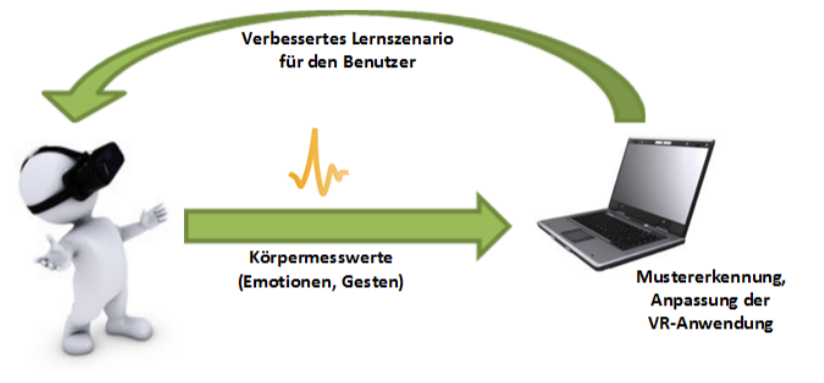
\includegraphics[width=12cm]{Images/elise_projektbeschreibung.png} 
\vspace{-0.3cm} 
\caption{Grobe {\"U}bersicht des Gesamtprojekts\cite{msckroenert}.}
\label{fig-elise} 
\end{figure}

Der Lehrstuhl Medizinische Informatik und Mikrosystementwurf entwickelt im Rahmen des Gesamtprojektes ein Sensorsystem, welches die Vital-, Elektroenzephalografie-, Elektrookulografie- und galavanische Hautreaktionwerte aufzeichnet. 
Diese werden dann vom Lehrstuhl f{\"u}r Mustererkennung ausgewertet. 
Die Lerninhalte der Hauptanwendung des ELISE-Projekts werden daraufhin an Emotionen und Gem{\"u}tslagen der Lernenden wie Gl{\"u}ck, Langeweile, Frustration auf Basis von biomedizinischer Daten angepasst, um so den individuellen Erfolg des Lernenden zu erh{\"o}hen.

% Unterkapitel
\subsection{Gliederung dieser Dokumentation} \label{gliederung-subsec}


Die Dokumentation ist in mehreren Teil gegliedert: eine Einführung, die Entwicklung des ersten Prototypen, die Entwicklung des zweiten Prototypen, die Entwicklung des dritten/finalen Prototypen und ein Schlussteil. \\

Einführung: \\

Die Dokumentation fängt mit einer Einleitung an, die den Hintergrund und die Motivation, die Elise Projektbeschreibung, die Gliederung dieser Dokumentation und den mit der Dokumentation übergebenen Anhang erläutert (geschrieben von Minas Michail). 
Der nächste Punkt ``Organisation'' beinhaltet zum einen die Verantwortungsbereiche der aufgeteilten Aufgaben innerhalb der Gruppe und  zum anderen wird erläutert wie und wann die Gruppentreffen stattgefunden haben (geschrieben von Artur Piet). 
Daraufhin werden die Grundlagen übermittelt, um späteres geschehen in der Dokumentation besser nach voll ziehen zu können. 
Der Punkt Grundlagen enthält die Definition von Emotionen (geschrieben von Arnaud Eric Toham Waffo), die Grundlagen der verwendeten Hardware und Software (geschrieben von Arnaud Eric Toham Waffo), die Grundlagen der verwendeten Sensoren und biophysiologischen Signale (geschrieben von Kevin Orth), die Grundlagen der Kommunikation zwischen den gewonnen Sensordaten und dem Board (geschrieben von Kevin Orth \& Jonas Pöhler), die Grundlagen der Mustererkennung (geschrieben von Artur Piet) und die Grundlagen zur Emotionserkennung (geschrieben von Artur Piet). 
Nach den Vermittlungen der Grundlagen \\

Entwicklung des ersten Prototypen: \\

Die Entwicklung des ersten Prototypen umfasst den Systementwurf und das Konzept der Hardware (geschrieben von Kevin Orth), die entwickelte Software zurKommunikation (geschrieben von Kevin Orth \& Jonas Pöhler), die Emotionsinduktion (geschrieben von Meryem Dural, Boris Kamdem \& Minas Michail), die Messreihe (geschrieben von Kevin Orth \& Artur Piet), die Musterkennung (geschrieben von Artur Piet) und die gewonnen Ergebnisse (geschrieben von Artur Piet). \\

Entwicklung des zweiten Prototypen: \\

Die Entwicklung des zweiten Prototypen umfasst den Systementwurf und das Konzept der Hardware und die modifizierte Software zur Kommunikation (beides  geschrieben von Kevin Orth \& Jonas Pöhler). 
Parallel zur Fertigstellung des zweiten Prototypen, lief die Entwicklung der Emotionsinduktion für den dritten Prototypen. \\

Entwicklung des dritten Prototypen: \\

Die Entwicklung des dritten Prototypen umfasst den Systementwurf und das Konzept der Hardware (geschrieben von Kevin Orth), die entwickelte Software zurKommunikation (geschrieben von Kevin Orth \& Jonas Pöhler), die Emotionsinduktion (geschrieben von Meryem Dural, Boris Kamdem \& Minas Michail), die Messreihe (geschrieben von Kevin Orth \& Artur Piet), die Musterkennung (geschrieben von Artur Piet) und die gewonnen Ergebnisse (geschrieben von Artur Piet). \\

Schlussteil: \\

Der Schlussteil beinhaltet das Kapitel Alternative Lösungen aufgeteilt in Kalibrierung (geschrieben von Jonas Pöhler) und Plan B (geschrieben von Meryem Dural) und eine Zusammenfassung (geschrieben von Arnaud Eric Toham Waffo) sowie einen Ausblick (geschrieben von Boris Kamdem).

% Unterkapitel
\subsection{Anhang}  \label{anhang-subsec}


Der Anhang enthält alle Dateien, die im Rahmen dieser Projektgruppe erstellt wurden, und wird in Form einer beigelegten CD-Rom zur Verfügung gestellt.
Bei diesen Dateien handelt es sich im Wesentlichen um die erstellten Eagle-Dateien (Schaltplan und Layout) die Dateien für den 3 Druck (Maske und Gehäuse) sowie den erstellten Code für den Mikrocontroller und die zu verarbeitende Software.
Zuletzt sind noch alle erstellten Anleitungen, für den Hardwareaufbau und die Versuchsdurchführung enthalten. Eine genaue Beschreibung der in den erwähnten Dateien behandelten Themen erfolgt in den nachfolgenden Kapiteln.
Auf der CD-Rom befinden sich im Ordner Senfemo-Anhang die folgenden Dateien:
\newline
-Eagle-Dateien aller drei Prototypen
\\
-Code für die Prototypen
\\
-Datenblätter der verwendeten Komponenten
\\
-Dateien für den 3D-Druck
\\
-diverse Anleitungen 



% 3 Organisation
\newpage
\section{Organisation} \label{organisation-0}
\todo[inline]{Verantwortlich: Artur \\}


Diese Projektgruppe des ELISE Projektes wir dem Lehrstuhl Medizinische Informatik \& Mikrosystementwurf und dem Lehrstuhl für Mustererkennung zugeordnet. \\

Die Gruppe wird von Dr.-Ing. Armin Grünewald, David Krönert und Frédéric Li geleitet. 
Innerhalb der Gruppe wurden dazu unabhändig ein Sprecher und ein stellvertretender Sprecher von den Gruppenmitgliedern gewählt. Als Projektgruppensprecher wurde Artur Piet und als Stellvertreter Jonas Pöhler ausgewählt. 
Diese Stellung ist jedoch nicht die eines Leiters mit Entscheidungs- und Weisungsbefugnissen. Die Sprecher sind also auf die Kooperationsbereitschaft der anderen Gruppenmitglieder angewiesen. 
Konkrete Aufgaben der Sprecher waren unter anderen das Verteilen von Verantwortungsbereichen auf alle Mitglieder, die Einführung von regelmäßigen Gruppentreffen um den Überblick über alle Fortschritte zu garantieren und die Übernahme möglichst aller organisatorischer Tätigkeiten (z.B. Messreihen organisieren, Beschaffungsprozesse koordinieren, usw.). \\

Die Laufzeit der Projektgruppe wurde auf etwa 1 Jahr gesetzt, wobei das Kick-Off Meeting am 23.10.2017 stattfand. Der geforderte individuelle Zeitaufwand aller Gruppenmitglieder entspricht der jeweils im Modulhandbuch des Studienganges definierten Leistungspunkte für die Projektarbeit, also 600 Stunden für Jonas Pöhler, Arnaud Eric Toham Waffo, Boris Kamdem, Kevin Orth, Meryem Dural sowie Minas Michail und 270 Stunden für Artur Piet. Es folgt ein Balkendiagramm mit den geforderten Stunden im Verlgeich zum tatsälichem Zeitaufwand. \\

\begin{figure}[h]
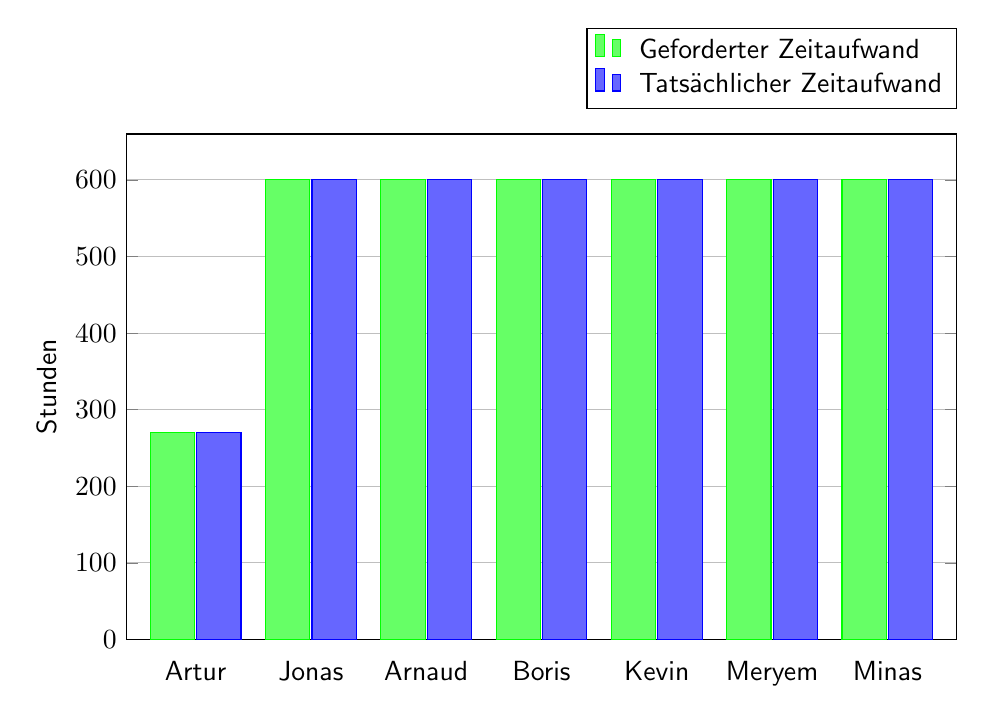
\begin{tikzpicture}
    \begin{axis}[
        width  = \textwidth,
        height = 8cm,
        major x tick style = transparent,
        ybar=2*\pgflinewidth,
        bar width=16pt,
        ymajorgrids = true,
        ylabel = {Stunden},
        symbolic x coords={Artur,Jonas,Arnaud,Boris,Kevin,Meryem,Minas},
        xtick = data,
        scaled y ticks = false,
        enlarge x limits=0.1,
        ymin=0,
        legend cell align=left,
        legend style={
                at={(1,1.05)},
                anchor=south east,
                column sep=1ex
        }
    ]
        \addplot[style={green,fill=green!60,mark=none}]
            coordinates {(Artur, 270) (Jonas,600) (Arnaud,600) (Boris,600) (Kevin,600) (Meryem,600) (Minas,600)};

        \addplot[style={blue,fill=blue!60,mark=none}]
             coordinates {(Artur,270) (Jonas,600) (Arnaud,600) (Boris,600) (Kevin,600) (Meryem,600) (Minas,600)};

        \legend{Geforderter Zeitaufwand,Tatsächlicher Zeitaufwand}
    \end{axis}
\end{tikzpicture} 
%\caption{Stundenaufwand: Vergleich zwischen gefoderten und tatsächlichen Zeitaufwand der Projektgruppenmitglieder.} 
\end{figure} 



\subsection{Verantwortungsbereiche}
Innerhalb der Projektgruppe (PG) war ein Ziel, dass jeder der Mitglieder "Experte" für einen Bereich wird. Damit haben wir die Verantwortung relativ gleichmäßig auf alle aufgeteilt. Dazu muss noch erwähnt werden, dass die Teammitglieder nicht nur ausschließlich die Aufgaben des jeweiligen Verantwortungsbereiches erlegibt habe. Es wurde sich vielmehr gegenseitig immer unterstützt und viel zusammengearbeitet. Die Verantwortungsbereiche haben sich mit der Zeit folgendermaßen aufgeteilt: \\

$ \bullet $ Artur Piet: Mustererkennung, 3D-Konstruktion und Sprecher der PG \\
$ \bullet $ Jonas Pöhler: Hardware, Webanbindung und Stellv. Sprecher der PG \\
$ \bullet $ Arnaud Eric Toham Waffo: Elektrodenauswahl \\
$ \bullet $ Boris Kamdem: Langeweile-Szenario und Fragebogen in VR \\
$ \bullet $ Kevin Orth: Komplette Hardware \\
$ \bullet $ Meryem Dural: Frustations-Szenario in VR \\
$ \bullet $ Minas Michail: Glücks-Szenario in VR \\


\subsection{Gruppentreffen}
Die wöchentliche Gruppentreffen finden immer Donnerstags ab 14:00 Uhr statt und beginnen in der Regel mit einer Update-Runde. Hierbei kommen alle Gruppenteilnehmer der Reihe nach dran und jeder erklärt kurz woran letzte Woche gearbeitet wurde, was die aktuellen Herausfoderungen und Probleme sind und was genau als nächstes geplant ist. Ziel ist es den Austausch und die Kommunikation unter den Teammitgliedern und den Projektleitern zu fördern, damit alle Teilnehmer auf dem selben Wissenstand sind, da einzelnen Aufgaben durchaus großen Einfluß auf Tätigkeiten von anderen Mitgliedern haben können. \\


% 4 Grundlagen
\newpage
\section{Grundlagen} \label{grundlagen-0}
\todo[inline]{Verantwortlich: Arnaud}

Mit diesem Kapitel werden Einblicke in die notwendige Grundlagen zur Realisierung unserer Arbeit gegeben. Zuerst werden wir uns mit der Thematik Emotion(Definition und Klassifikation) beschäftigen. Im Weiteren werden ``Virtual Reality'' ( beziehungsweise HTC Vive VR-Brille) genauer erklärt. Ebenfalls kommt eine Erläuterung der Sensoren und Biophysiologische Signale, welche für unsere Arbeit von Bedeutung sind. Näher wird auf die Kommunikation zwischen verschiedenen Sensoren eingegangen.Dazu kommt auch eine Erklärung wie die Datenerfassung(Messreihe) stattfinden sollte
 Danach befassen wir uns mit der Grundlagen der Mustererkennung. Ein Berichtsteil über die ``Emotion Recognition chain'' schließt das Kapitel ``Grundlagen'' ab.


% Unterkapitel
\subsection{Definition von Emotionen} \label{definition-emotionen-sec}


\todo[inline]{Verantwortlich: Arnaud}

% Unterkapitel
\subsection{Virtual Reality (VR)} \label{grund-vr}

\todo[inline]{Verantwortlich: Arnaud, Boris}

Virtuelle Realität wird helfen, besser den Emotionen zu erliegen, die wir uns wünschen. Es kann als Variante für die üblichen Modelle gesehen werden, bei denen Testpersonen vor Bildschirmen mit emotionalen Videos platziert werden. 

% Unterkapitel
\subsection{Sensoren und biophysiologische Signale zur Emotionserkennung} \label{grund-sensoren}


Emotionen aus biophysiologischen Signalen abzuleiten ist eine neuere und weitere Entwicklung.
Durch das zentrale Nervensystem gesteuerte biologische Reaktionen des Körpers sind Emotionen nur teilweise oder gar nicht der Kontrolle unseres Bewusstseins unterlegen.  Aus diesem Grund besteht eine direkte und unverfälschte Verbindung zu unseren Emotionen, die uns die Möglichkeit gibt, einen unmittelbaren Einblick in den menschlich-affektiven Zustand zu gewähren. Bildgebende Verfahren sind dabei immer noch, insbesondere die nichtinvasiven Methoden der funktionellen Magnetresonanztomographie, unabdingbar, um einen Blick in das emotionsverarbeitende menschliche Gehirn zu ermöglichen.  Jedoch überwiegen in der Emotionsforschung die Nachteile der Magnetresonanztomographie durch zum Beispiel Klaustrophobie, Kosten, Dauer, Verwackelgefahr und Lautstärke, wodurch neue Systeme zur Kompensierung der Nachteile durch neue Sensorik entwickelt werden müssen. Unser Körper sendet die gemessenen Signale ohne Unterbrechung, so dass man einen kontinuierlichen Signalstrom erhält. Jedoch reagiert der Mensch sehr individuell auf Emotionen, was es sehr schwierig macht, allgemeingültige Regeln zu finden. Unbekannte Erlebnisse werden viel eindringlicher erlebt, eher bekannte Situationen im Gegenzug schwächer. Auch die Umgebung, das Alter und die Erfahrungen haben einen wesentlichen Einfluss auf die Empfindung. Als Biosignale werden alle physikalisch messbaren und kontinuierlich oder nahezu kontinuierlich registrierbaren Körperfunktionen bezeichnet. Hierbei unterscheidet man direkte bioelektrische Signale (z.B. Herzschlag, Hirnaktivität), indirekte bioelektrische Signale (z.B. Hautleitfähigkeit) und nicht elektrische Signale (z.B. Blutdruck, Atemfrequenz). Für die Aufzeichnung des Korpus der Emotionsforschung liegen Signale der Sensoren Körpertemperatur, BVP (Blood Volume Pulse), SpO2 (Sauerstoffsättigung), GSR (Galvanic Skin Response), EEG (Elektroenzephalografie) und EOG (Elektrookulografie) vor.

% Unterkapitel
\input{Part-0/4-Grundlagen/3-Sensoren/1-temperatur}

% Unterkapitel
\input{Part-0/4-Grundlagen/3-Sensoren/2-bvp}

% Unterkapitel
\input{Part-0/4-Grundlagen/3-Sensoren/3-spo2}

% Unterkapitel
\input{Part-0/4-Grundlagen/3-Sensoren/4-gsr}

% Unterkapitel
\input{Part-0/4-Grundlagen/3-Sensoren/5-eeg}

% Unterkapitel
\input{Part-0/4-Grundlagen/3-Sensoren/6-eog}

% Unterkapitel
\input{Part-0/4-Grundlagen/3-Sensoren/7-ad-wandler}

% Unterkapitel
\input{Part-0/4-Grundlagen/4-Kommunikation/1-kommunikation}




% Unterkapitel


% Unterkapitel
\input{Part-0/4-Grundlagen/5-Mustererkennung/1-grundlagen-mustererkennung}


% Unterkapitel 
\input{Part-0/4-Grundlagen/5-Mustererkennung/2-emotion-recognition-chain}





% 5 SOA Analyse
\newpage
\section{State-of-the-Art Analyse} \label{soa-0}


Die Detektion von Emotionen kann auf unterschiedlichste Art erfolgen. In der Literatur wird neben der Verarbeitung von Biosignalen mittlerweile häufig auf eine Detektion durch Kameras oder durch die Analyse von Sprache gesetzt.(vgl. \cite{soa1, soa2, soa3, soa4}) \\

Die Analyse mittels einer Kamera und der Aufnahme von Gesichtsmimik oder Augenbewegung war in der vorliegenden Arbeit nicht möglich, da die HTC Vive die der Proband während des Experimentes trägt, einen Großteil des Gesichtes und damit die Mimik wie auch die Augen verdeckt. Eine Interaktion mit dem Probanden mittels Sprache war ebenfalls nicht vorgesehen. Dementsprechend blieb nur die Möglichkeit der Detektion von Emotionen mittels Biosignalen. Hierbei wird in der Literatur vor allem die Atemfrequenz, die Hautleitfähigkeit, die elektrische Herzaktivität, die EEG Ableitung und die EOG Ableitung heran gezogen.(vgl. \cite{soa5, soa6, soa7, soa8}) \\

Zur Klassifizierung der Emotionen werden in der Literatur unterschiedliche Techniken verwendet. In neuerer Zeit konzentriert sich die Forschung dabei auf Machine Learning gestützte Ansätze.(vgl. \cite{soa9, soa10}) Dabei wird zwischen supervised und unsupervised Modellen unterschieden. Bei den unsupervised Modellen wird insbesondere Sequential Floating Forward Search und k-Nearest Neighbour (k-NN) benutzt. Hierbei handelt es sich um Techniken zur Selektion relevanter Features beziehungsweise zur Klassifizierung von Features durch Gruppenbildung.  Auf der Seite der supervised Modelle sticht vor allem die Nutzung der Support Vecotor Machine (SVM) hervor.(vgl. \cite{soa11, soa12, soa13}) Hierbei wird wie bei allen supervised Modellen ein Datensatz mit Labels genutzt um das Modell auf die zugrunde liegende Datenmenge zu trainieren. 




% Part 1
\newpage
\renewcommand{\headrulewidth}{0.5pt}
\fancyhf{} \cfoot{\thepage} \rhead{\leftmark \hspace{0.2cm} PART I} % Header Part 1
\part{Erster Prototype}
\addtocontents{toc}{\protect\mbox{}\protect\hrulefill\par}


% 1 Systementwurf
\section{Systementwurf und Konzept} \label{systementwurf-sec}
\todo[inline]{Verantwortlich: Kevin, Jonas}



% Unterkapitel 
\subsection{Anforderungen} \label{anfoderungen-1}

Auf Grundlage der Ziele des Forschungsprojektes ELISE und dem Sichten und Vergleichen von mehr als 30 wissenschaftlichen Veröffentlichungen der letzten 15 Jahre, ergeben sich bestimmte
Anforderungen für den Entwurf eines eigenen Emotionserkennungssystems. Einige wissenschaftliche Veröffentlichungen sind dabei nicht außer Acht zu lassen. Die Foscher von T.
Sharma, S. Bhardwaj und H. B. Maringanti haben in ihrer Veröffentlichung Emotion Estimation
using Physiological Signals versucht, mit Hilfe von GSR, Herzschlagrate,
BVP und der Temperatur Aufschluss über die Emotionen Zorn, Angst, Freude und Traurigkeit
durch Stimulation verschiedener Songs und Videos zu erhalten. Sie erforschten, in
welchen Fällen sich die Körperleitfähigkeit je nach emotionalem Ausdruck unterschiedlich
verhält. H. F. Garcia, A. A. Orozco und M. A. Alvarez versuchten in ihrer Arbeit Dynamic
physiological signal analysis based on Fisher kernels for emotion recognition durch unterschiedliche Klassifizierungsmodelle, die Signale von EEG, EOG, EMG (Elektromyografie),
GSR, Atmung und Temperatur zu analysieren. Dafür wurden 32 Probanden,
die ein 40-minütiges Video mit Musikausschnitten ansahen, aufgezeichnet und ausgewertet.
Durch ein automatisches Regressionsprozess-Modell verbesserten sie dynamische Merkmale
und weitere aufgezeichnete Signale für eine weiterführende Auswertung.
Die Emotionserkennung erfolgte bis vor einigen Jahren in Verbindung mit zusätzlichen Kameras
und Software zur Gesichtsmimik-Erkennung oder Stimmerkennung, nicht jedoch mit
einer reinen Aufnahme von Körpermesswerten. In ELISE sollen insbesondere die lernrelevanten Emotionen Langweile, Frustration, Verwirrung sowie Engagement und Freude erkannt
werden. Die Hardware-Architektur muss auch in diesem Fall wieder das Ziel erfüllen, dass
das Gefühl der Immersion nicht gestört wird. Das heißt, dass das System zur Erkennung von
lernrelevanten Emotionen an möglichst wenigen Stellen am Körper mit zusätzlicher Sensorik
angebracht wird.
Auf Basis der Literaturrecherche, wie in der Bibliographie ausgewiesen, sind folgende Sensoren
zur Aufnahme der lernrelevanten Emotionen ausgewählt worden:

• Gehirnaktivität (EEG)
• Augenbewegung (EOG)
• Blutvolumenpuls (BVP)
• Sauerstoffsättigung im Blut (PPG)
• Hautleitfähigkeit (GSR)
• Körpertemperatur

Da die Sensorwerte zum Mikrocontroller aufgrund ihres räumlichen Abstandes über den
Bus übertragen werden, unterliegen diese Werte den Zeitanforderungen des Datenbusses.
Hier ist zu überprüfen, welches Buskonzept den Zeitanforderungen gewachsen ist.
Um den Aufwand für den Benutzer gering zu halten und die Immersion nicht zu stören,
wird versucht, die Sensorik direkt an der VR-Brille anzubringen. Für die EEG- und
EOG-Sensoren ist dies sowieso notwendig, da diese Messungen lediglich am Kopf stattfinden
können. Zudem soll das Endsystem echtzeitfähig sein, um in der späteren Anwendung
Änderungen und Fluktuationen der Emotionen erkennen zu können und die Schulungen auf
den Lernenden anzupassen. Das Emotionserkennungssystem soll mobil anwendbar sein, da
neuere Versionen der HTC Vive VR-Brille in Zukunft den kabellosen Betrieb unterstützen.
Auch aus diesem Grund ist die Kompaktheit, Energieeffizienz und die Datenübertragung der
einzelnen Sensoren und die Datenübertragung des späteren Gesamtsystems, die ebenfalls
kabellos stattfinden soll, von großem Interesse. Eine mögliche Stelle zur Unterbringung des
Gesamtsystems wäre am Hinterkopf des Probanden, da dort der nötige Platz vorhanden ist
und erforderliche Befestigungsstellen am Kopfband der HTC Vive von Vorteil sind.



% Unterkapitel 
\subsection{Konzept} \label{konzept-1}

Auf Abbildung 1 kann man das Konzept der Architektur erkennen, Dies ist zur besseren Anschauung stark vereinfacht. Hierbei bildet der Mikrocontroller das zentrale Element, welches die einzelnen Sensoren anbindet, steuert und die Messsignale grob zur besseren Auswertung verarbeitet. Zur besseren und möglichst in Echtzeit stattfindeten Verarbeitung werden die Daten an einen externen Rechner weitergeleitet. In der Abbildung findet diese Weiterleitung Drahtlos mittels Bluetooth statt. Es wurden in den verschiedenen Prototypen für diese Zwecke sowohl Bluetooth als auch WLAN verwendet. Für die Teilsysteme EEG und EOG wurden schon einfache Physische Filter auf den Leiterplatten vorgesehen, welche die analogen Signale vorberarbeiten, bevor dies von einem AD-Wandler digitalisiert werden. Da die Elektroden für die EEG und EOG Messung nur am Kopf angebracht werden können, empfiehlt es sich die übrigen festgelegten Werte ebenfalls am Kopf zu messen. Um die Messung für möglichst viele Personen mit unterschiedlichen Kopfformen zu ermöglichen wurde zuerst ein elastisches Kopfband und später eine flexible Maske verwendet. All dies wurde für eine spätere Verwendung mit (unter) einer VR-Brille designet. 





% Unterkapitel
\subsection{Hardwareauswahl} \label{hardwareauswahl-1}

Bei der Wahl der richtigen Hardware zur Aufnahme, Verarbeitung und Weiterleitung von
biomedizinischen Signalen, sind die reinen Hardwarekosten von untergeordneter Bedeutung.
Jedoch sollte das Budget für das spätere Gesamtsystem einen gewissen Rahmen nicht überschreiten,
um auch die aufkommenden Endkosten in Verbindung mit einer VR-Brille und der
benötigten Hardware zur Darstellung der Lerninhalte in einem gewissen Rahmen zu halten.
Die Bandbreite der angebotenen Systeme von unterschiedlichen Mikrocontrollern ist dabei
sehr groß. Zu Beginn einer geeigneten Neubeschaffung sollten, wie bei jedem IT-Projekt, die
zuvor genannten Anforderungen an das System betrachtet werden und daraus Auswahlkriterien
für die geeignete Hardware gewählt werden.

% Unterkapitel 
\input{Part-1/1-Systementwurf/3-Hardwareauswahl/1-auswahlkriterien}

% Unterkapitel 
\input{Part-1/1-Systementwurf/3-Hardwareauswahl/2-festlegung-hardware}



% Unterkapitel
\subsection{Hardwarearchitektur} \label{hardwarearchitektur-subsec}



% Unterkapitel
\input{Part-4/1-Systementwurf/4-Hardwarearchitektur/1-gsr}

% Unterkapitel
\input{Part-4/1-Systementwurf/4-Hardwarearchitektur/2-temperatur}

% Unterkapitel 
\input{Part-4/1-Systementwurf/4-Hardwarearchitektur/3-pulsoximeter}

% Unterkapitel 
\input{Part-4/1-Systementwurf/4-Hardwarearchitektur/4-eeg}

% Unterkapitel 
\input{Part-4/1-Systementwurf/4-Hardwarearchitektur/5-eog}

% Unterkapitel
\input{Part-4/1-Systementwurf/4-Hardwarearchitektur/6-datenuebertragung}



% Unterkapitel 
\subsection{Programmierung} \label{programmierung-subsec}

Die Programmierung des dritten Prototypen basiert im wesentlichen auf der des zweiten Protoypen, da sich in Bezug auf die Hardware nur die GSR-Schaltung geändert hat. Wie auch bei vorherigen Prototypen erfolgte die Programmierung mit Hilfe der Arduino Plattform und der durch die Hersteller schon zur Verfügung gestellten Bibliotheken.





% Unterkapitel 
\subsection{Aufnahme der {\"u}bertragenen Daten} \label{aufnahme-daten-subsec}

Beim dritten Prototypen wurden die Daten wieder drahtlos übertragen. Im Gegensatz zum ersten Prototypen kam hier aber nicht mehr ein Bluetooth-Modul zum Einsatz, sondern das im ESP32 integrierte WLAN-Modul. In den mit diesem Prototypen durchgeführten Messungen wurden die Daten mittels WireShark aufgenommen und abgespeichert. Diese Daten wurden später zur Datenanalyse in eine CSV-Datei umgewandelt. Zur Übertragung wurde das zuvor schon beschriebene UDP-Protokoll  verwendet. An dieser Stelle sei noch einmal Erwähnt, das alle Daten mit einer Abtastrate von 250 Samples pro Sekunde gemessen wurden. Die einzige Ausnahme hier ist die Temperatur, die lediglich mit einer Rate von 3,3 Samples pro Sekunde gemessen wurde. 




% 2 Realisierung
\newpage
\section{Realisierung} \label{realisierung-sec}


Für den ersten Versuch mit Testpersonen wurden die Experimente zur Emotionsinduktion zu einem Gesamtexperiment verbunden. Dabei wurde darauf geachtet einen möglichst automatisierten Testablauf zu erreichen, so dass die Testperson möglichst unbeeinflusst von äußeren Reizen oder den Aktionen des Testleiters bleibt. Dazu wurde eine automatisierte Webanwendung programmiert, die der Versuchsperson alle Anweisungen und Experimente präsentiert (siehe Abbildung \ref{fig:screen_soft1}). Der Versuchsleiter wiederum kann durch eine, ebenfalls webbasierte, Kontrollkonsole Einfluss auf das Experiment nehmen, in dem er zum Beispiel den Ablauf stoppen oder Schritte überspringen kann (siehe Abbildung \ref{fig:screen_soft1}).\\

Die Ablaufkontrolle erfolgt über den Flask Webserver, der die Website darstellt. Zur Steurung können einfach URLs auf dem Server mittels einer GET bzw. POST Anfrage aufgerufen werden und so Steuerbefehle übermittelt werden. \\

Die Bilder, die dem Probanden angezeigt werden, wie auch die Spiele, die er spielen soll, sind nahtlos in die Website eingebettet. Dies ist möglich, dadurch, dass es sich zum einen um eine Javascript Anwendung und zum anderen um eine Flash Anwendung handelt. Die Flash Anwendung wurde zur einfacheren Handhabung so präpariert, dass das Menü entfernt wurde und das Spiel direkt mit dem ersten Level beim Laden startet. \\

\begin{figure}[h]
    \centering
\begin{minipage}[t]{0.9\textwidth}
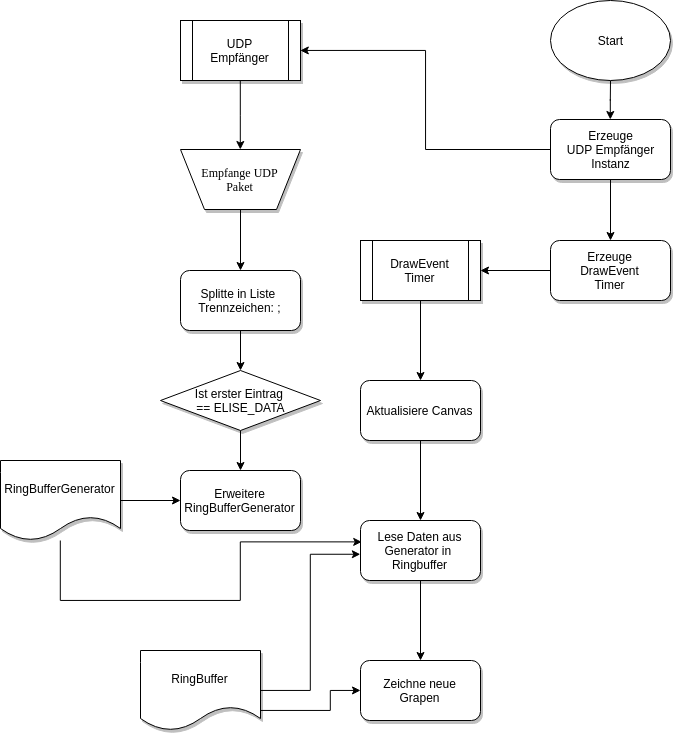
\includegraphics[width=\textwidth]{Images/ablauf_anzeige.png}
\end{minipage}
    \caption{Screenshot der Supervisor Ansicht}
    \label{fig:screen_soft1}
\end{figure}





% 3 Emotionsinduktion
\newpage
\section{Emotionsinduktion} \label{emotionsinduktion-sec}
\todo[inline]{Verantwortlich: Minas}


% Unterkapitel
\subsection{Ablauf} \label{ablauf-1}


\todo[inline]{Verantwortlich: Minas}


Der Ablauf der Emotionsinduktion lief wie folgt ab:

\begin{itemize}
\item[1.] Gl{\"u}ck (PowerPoint) $\rightarrow$ Kapitel 7.3.1
\item[2.] Langeweile (Video) $\rightarrow$ Kapitel 7.3.2
\item[3.] Frustration (Flashgame) $\rightarrow$ Kapitel 7.3.3
\item[4.] Langeweile (Spiel im Browser) $\rightarrow$ Kapitel 7.3.2
\end{itemize}

Nach jedem Szenario folgte ein sich automatisch {\"o}ffnender Fragebogen zum Szenario. 
Der Wechsel zwischen den Szenarien musste manuell statt finden.

% Unterkapitel 
\subsection{Fragebogen} \label{fragebogen-4}


\todo[inline]{Verantwortlich: Boris\\
- add picture of VR questionare (both dominat emotions and circumplex)}

F{\"u}r dieses Prototyp wurden zwei Arten von Frageb{\"o}gen benutzt. 
Der erste Typ ist sehr {\"a}hnlich mit dem von der zweite Prototyp. Es enth{\"a}lt in dem informativen Teil einen Text, wo es beschrieben wird, wie der Fragebogen ausgef{\"u}llt werden soll. Der andere Teil besteht aus vier Dropdown-Boxen von dreizehn Optionen, die zw{\"o}lf verschiedene Emotionen und einen als null oder neutral geltenden Zustand enthalten. Jede Dropdown-Box entspricht ein Viertelzeit der Szenario. Es soll zwischen die Optionen jeder Dropdown-Box gew{\"a}hlt werden, welche Emotion es am st{\"a}rksten empfindet wird, je nachdem, wann man es f{\"u}hlte, d.h. ob es das erste, zweite, dritte oder letzte Quartal der Zeit des Videos war, um die Emotion zu bew{\"a}ltigen. Unten gibt es ein Button wo man dr{\"u}cken kann, wenn man fertig ist. Allerdings hat man auch die M{\"o}glichkeit seine Wahl zu {\"a}ndern, auch wenn man sich schon im n{\"a}chsten Schritt befindet, indem man in diesem n{\"a}chsten Schritt auf den Zur{\"u}ck-Button dr{\"u}ckt und die gew{\"u}nschten {\"a}nderungen vornimmt. Hierf{\"u}r wird ein Widget Blueprint erstellt, die vier Dropdown-Boxen mit dem gew{\"u}nschten Anzahl an Optionen hinzugef{\"u}gt und die Labels von der unterschiedlichen Optionen der Dropdown-Boxen definiert. Ein Button ``next'' wird auch erstellt um zum n{\"a}chsten Fragebogen zu navigieren. Es wird auch eine zwischen Speicherungsfunktion in ein anderes Skript definiert, die hier aufgerufen wird, um die {\"a}nderung auch nach das dr{\"u}cken von dem ``next'' Button zu Speichern. Dabei wird vier Variablen definiert und die Werte von der gew{\"a}hlten Optionen werden ihnen zugewiesen. \\



\begin{figure}[H] \centering
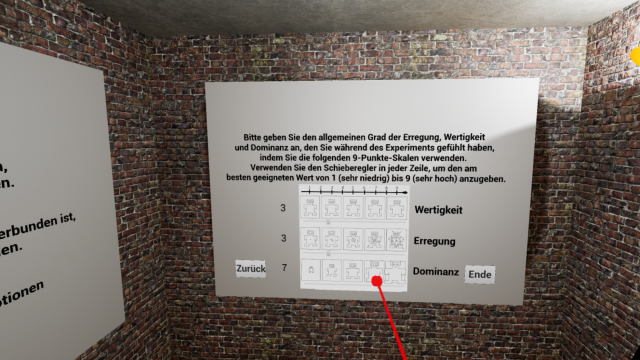
\includegraphics[width=\textwidth]{Images/Fragebogen_3.png} 
\caption{ Bild des Fragebogen-Teils, entsprechend dem circumplex-Modell. } 
\label{fig:fragenbogen4} \end{figure}



Der zweite Typ {\"a}hnelt dem ber{\"u}hmten Modell von James Russels ``circumplex'' \cite{russel_1980}. Es ist ein klassisches Modell mit einer kreisf{\"o}rmigen Struktur, die auf zwei senkrechten Diagonalen ruht. Die vertikale Achse, die die Erregung darstellt, und die horizontale Achse, die die Valenz darstellt. Das Zentrum des Kreises stellt eine neutrale Valenz und ein mittleres Erregungsniveau dar. Andere Emotionen werden auf jeder Ebene des Kreises dargestellt.  Hier wird ein weniger bekanntes Modell verwendet, das ``Self Assessment Manikin'' (SAM). Es besteht aus drei Reihen mit je f{\"u}nf Piktogrammen. Diese Piktogramme stellen den Zustand eines Gesichts nach verschiedenen Arten von Emotionen dar. So repr{\"a}sentiert der erste Bereich die Wertigkeit, der zweite die Erregung und der dritte die Dominanz. Eine Erkl{\"a}rung zu jedem dieser Begriffe ist ebenfalls neben dem Fragebogen enthalten, um die Testpersonen {\"u}ber diese W{\"o}rter aufzukl{\"a}ren.  Bei jeder Avatar und in der Mitte jeder der beiden Avatar befindet sich ein Checkbox.  So muss man f{\"u}r jede Zeile das Checkbox ausw{\"a}hlen, das ihrem emotionalen Zustand am besten entspricht. Man kann nur ein Checkbox pro Zeile markieren und man hat auch die M{\"o}glichkeit wie bei dem ersten Model seine Wahl zu {\"a}ndern. Es kann einfach mit Branch-Bedingungen realisieren werden.  Diese werden auch in eine Widget Blueprint wie f{\"u}r das erste Modell gemacht. Es gibt auch wieder die zwischen Speicherungsfunktion und das Button ``next''. Was neues hier kommt ist das Button ``back'' um wieder zum ersten Fragebogen zu navigieren. 



\begin{figure}[H] \centering
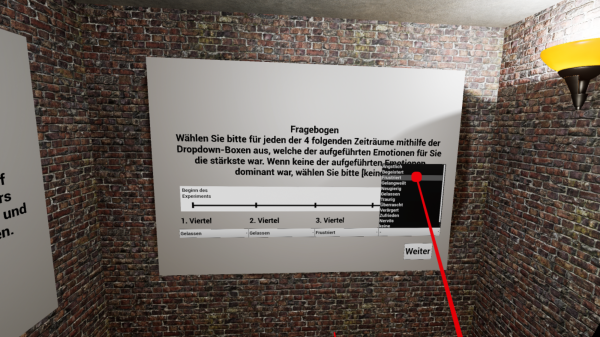
\includegraphics[width=\textwidth]{Images/Fragebogen_1.png} 
\caption{ Bild des Fragebogen-Teils, wo die dominierenden Emotionen abgefragt werden. } 
\label{fig:fragenbogen1} \end{figure}

% Unterkapitel 
\subsection{Szenarien} \label{szenarien-subsec}

\todo[inline]{Verantwortlich: Meryem}

% Unterkapitel 
\input{Part-1/3-Emotionsinduktion/3-Szenarien/1-glueck}

% Unterkapitel 
\input{Part-1/3-Emotionsinduktion/3-Szenarien/2-langeweile}

% Unterkapitel 
\input{Part-1/3-Emotionsinduktion/3-Szenarien/3-frust}


% 4 Messreihe
\newpage
\todo[inline]{Kevin, Artur}




% 5 Mustererkennung
\newpage
\section{Mustererkennung} \label{mustererkennung-sec}

\todo[inline,color=green!40]{Verantwortlich: Artur\\
- RfP}

In diesem Kapitel werden alle Schritte entlang der ERC (vgl. Kapitel \ref{emotion-recogniton-chain}) konkretisiert und es wird detailreich beschrieben, wie wir vorgegangen sind. \\


% 1 Datenerfassung
\subsection{Datenerfassung} \label{datenerfassung-1}


In Kapitel \ref{messreihe-1-sec} wurde das verwendete Datenset bereits detailiert beschrieben, sodass hier darauf verzichtet wird. \\

% 2 Vorverarbeitung
\subsection{Vorverarbeitung} \label{vorverarbeitung-1}

Wie bereits in Kapitel \ref{vorverarbeitung-0} beschrieben, ist das Ziel der Vorverarbeitung die ”Verbesserung” der Daten f{\"u}r die nachfolgenden Schritte der ERC.
Im Rahmen des ELISE Projektes wurden Normalisierungstechniken auf dem gesamten Datensatz angewendet. 
Wir haben insbesondere die Standardnormalisierung verwendet, welche den Mittelwert der Daten auf Null setzt und die Einheitsvarianz ergibt \cite{grus15}. 
Die Formel f{\"u}r die Standardnormierung lautet:
\begin{equation} 
\Large{ {x'={\frac {x-{\overline {x}}}{\sigma }}} } 
\label{equ:norm} \end{equation} %\vspace{0.5cm}

wobei $ x $ ein Datenpunkt eines Sensorkanales, $ \overline{x} $ ist der Durchschnitt der Gesamtheit f{\"u}r diesen Sensorkanal und $ \sigma $ ist die entsprechende Standardabweichung. \\

% 3 Segmentation
\subsubsection{Segmentation} \label{segmentation-0}

Ziel dieses Schrittes ist es, Teile von Daten zu identifizieren, welche wichtige Informationen über die zu erkennenden Emotionen enthalten. 
Dies geschieht durch Filtern der Daten und Ausschließen von Segmenten, die für das Klassifizierungsproblem nicht relevant sind.
Zusätzlich wird die zu verarbeitende Datenmenge reduziert, indem Segmente eines Zeitfensters fester Größe aus den Daten extrahiert werden.
Diese Vorgeheisweise ist heute in der Praxis besonders wichtig, da sonst hardwarebedingte Einschränkungen die zu verarbeitende Datenmenge begrenzen könnten. \\

% 4 Merkmalsextraktion
\subsection{Merkmalsextraktion} \label{merkmalsextraftion-1}

Wie bereits in Kapitel \ref{merkmalsextraktion-subsubsec} beschrieben, ist das Ziel der Merkmalsextraktion Charakteristiken und Merkmale in den Daten zu finden, die für das
Klassifizierungsproblem von möglichst hoher Relevanz sind. Im Rahmen des ELISE Projektes haben wir verschiedene Vorgehensweisen angewendet. Im den folgenden Unterkapiteln werden diese vorgestellt. \\



% Unterkapitel 
\subsubsection{Handgefertigte Merkmale} \label{hc-features-1}
Der handgefertigten Merkmal Ansatz (enlg. "hand-crafted features approach") besteht in der Berechnung relativ einfacher Merkmale von denen vermudetet wird, dass sie für das Klassifizierungsproblem der Eingangssignale relevant sein können. Diese Vorgehensweise hat den Vorteil des einfachen Aufbaus als auch der relativ geringen benötigten Rechenleistung, wobei potentiell gute Klassifizierungsergebnisse erwarten werden. \\


Obwohl frühere Forschungsarbeiten schon handgefertigte Merkmale zur Emotionserkennung unter mithilfe physiologischer Signale getestet haben (vgl. \cite{martinez_ieee_2013}), wurde dieser Ansatz noch nie für die Erkennung dieser spezifischen Emotionen unter Verwendung dieser Kombination von Sensoren getestet.
Zusätzlich haben wir zuerst handgefertigte Merkmale getestet, um ein Basisergebnis zu liefern, mit der die Ergebnissen der anderen Ansätze vergleichen werden können.
Handgefertigte Merkmale sind in der Regel entweder einfache statistische Werte, Fourier-basierte oder selbstentwickelte Merkmale sein, die aufgrund von Vorkenntnissen der Daten verwendet werden. 
Diese Arbeit wurden statistische, Fourier-basierte und selbstentwickelte Merkmale getestet. \\

\textbf{Statistische Merkmale \\}
Die Tabelle \ref{tab:statistische} fasst die elf verschiedenen und in der Studie verwendeten statistischen Merkmale zusammen. Wir bezeichnen $\mathbf{x} = (x_1, x_2, ...., x_T) $ als Vektor, der die in einem Datenzeitfenster der Länge $T$ enthaltenen Sensorwerte für einen Sensorkanal darstellt. 


\begin{table}[h]
\begin{tabular}{| l | p{12.5cm} |}
\hline
    \textbf{Merkmalname}     &  \textbf{Definition}  \\ \hline
    
    Durchschnitt         & \vspace{0.01cm}
    $ mean(\mathbf{x}) =$ \Large{$\frac{1}{T} \sum_{k=1}^T (x_k) $} \\[0.5cm] \hline 
    
    Standard-Abweichung        & \vspace{0.01cm}
    $ \sigma(\mathbf{x}) =$ \Large{$ \sqrt{ \frac{1}{T} \sum_{k=1}^{T}{(x_k - \mu)^{2}} } $ } \\[0.5cm] \hline
    
    Maximum                   & \vspace{0.01cm}
    $ max(\mathbf{x}) = \max(x_{1},x_{2},\dots ,x_{T}) $
    \\[0.5cm] \hline
    
    Minimum                   & \vspace{0.01cm}
    $ min(\mathbf{x}) = \min(x_{1},x_{2},\dots ,x_{T}) $
    \\[0.5cm] \hline
    
    Amplitude                 & \vspace{0.01cm}
    $ A(\mathbf{x}) = max(\mathbf{x}) - min(\mathbf{x}) $ 
    \\[0.5cm] \hline
    
    25/50/75\% Perzentil      & Wert einer Menge, unter dem 25/50/75\% der Werte aus der Menge fallen. \\ \hline
    
    Interquartiler Bereich    & Differenz zwischen dem 75. und 25. Perzentil.
    \\ \hline
     
    Schräge                   & \vspace{0.01cm}
    $ \gamma _{1}(\mathbf{x}) = \operatorname{E}$ \Large{$\left[\left({\frac {X-\mu }{\sigma }}\right)^{3}\right]$ \normalsize{$=$} ${\frac {\mu _{3}}{\sigma ^{3}}}$ \normalsize{$=$} ${\frac {\operatorname {E} \left[(X-\mu )^{3}\right]}{ (\operatorname {E} \left[(X-\mu )^{2}\right])^{3/2}}}$ \normalsize{$=$} ${\frac {\kappa _{3}}{\kappa _{2}^{3/2}}} $} \vspace{0.2cm}
    \\[0.3cm] \hline
     
    Kurtosis                  & \vspace{0.01cm}
    $ \operatorname {Kurt}[\mathbf{x}] = \operatorname{E} $ \Large{$\left[\left({\frac {X-\mu }{\sigma }}\right)^{4}\right]$ \normalsize{$=$} ${\frac {\mu _{4}}{\sigma ^{4}}}$ \normalsize{$=$} ${\frac {\operatorname {E} [(X-\mu )^{4}]}{(\operatorname {E} [(X-\mu )^{2}])^{2}}} $} \vspace{0.2cm}
    \\[0.3cm] \hline
\end{tabular} 
\caption{Statistische Merkmale, die im Rahmen des ELISE-Projektes verwendet wurden. } \label{tab:statistische}
\end{table} 


\textbf{Fourier-basierte Merkmale \\}
\todo[inline]{Artur: \\
- Muss ich noch schreiben $\rightarrow$ Warten auf Julian's Antwort. \\}


\textbf{Selbstentwickelte Merkmale \\}
Es wurden zwei eigene Merkmale definiert: Nulldurchgang (engl. "zero crossing") und Anzahl der Spitzen (engl. "number of peaks"). Im Folgendem werden diese beiden Merkmale detailiert beschrieben. \\

Das Nulldurchgang-Merkmal zählt die Häufigkeit, mit der das Signal eines Sensorkanals in einem Zeitfenster die Nulllinie überschreitet.
Alle Sensorsignale wurden durch Normierung verarbeitet (vgl. Kapitel xxx) und damit wurden alle Mittelwerte auf Null zentriert.
Um zu vermeiden, dass Rauschen entlang der Nulllinie in dem Merkmal gezählt wird, wird nur ein Nulldurchgang in einer bestimmten Zeitspanne gezählt. \\


Das Spitzenzähler-Merkmal bestimmt die Anzahl von loklanen Hochpunkten im Zeitsignal.
Alle lokalen Maximen sind durch einen Onset (Startpunkt), eine Spitze und einen Offset (Endpunkt) gekennzeichnet (vgl. Abbildung \ref{fig:peaks}). 
Jedes Vorkommen einer Onset/Offset-Paarung wird hierbei als Spitze gezählt.
Onsets, Spitzen und Offsets werden durch die folgenden Operationen identifiziert \cite{BSc_Gouverneu}:

\begin{itemize} %[noitemsep]
  \item Ein Onset wird bestimmt, wenn der Wert des Signals an diesem Punkt nicht negativ ist und die Differenz zwischen ihm und dem nächsten größer als ein vordefinierter Schwellenwert (engl. "threshold") ist.

  \item Ein Offset wird bestimmt, wenn der Wert des Signals kleiner als der Wert des zuletzt gesetzten Onsets ist.

  \item Das lokale Maximum zwischen einem Onset und Offset wird als Spitze bezeichnet.
\end{itemize} \vspace{0.2cm}


\begin{figure}[h] \centering{
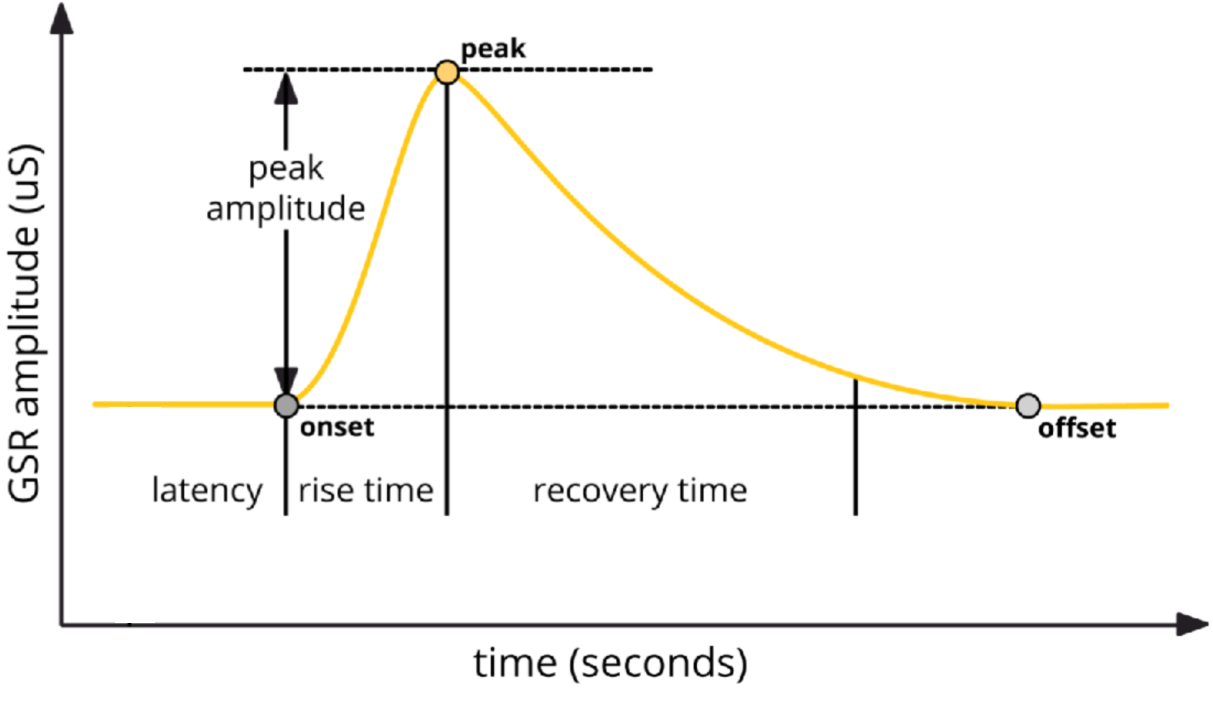
\includegraphics[width=11cm]{Images/peaks.png}}
\caption{ Spitzenzähler: Onset (Startpunkt), Spitze und Offset (Endpunkt). Jedes Paar von Onset/Offset erhöht die Anzahl der Spitzen um eins.} 
\label{fig:peaks} \end{figure} \vspace{0.5cm}


Jedes handgefertigte Merkmal wird auf einem Zeitfenster von Daten für jeden Sensorkanal unabhängig voneinander angewendet. 
Jedes Zeitfenster ist daher 117 Merkmalen zugeordnet (9 Sensorkanäle multipliziert mit 13 Merkmalen). \\





% Unterkapitel 
\subsubsection{Codebook Approach} \label{ca-1}


Die bisherige Methodik mit handgefertigten Merkmalen ist klassisch für den überwachten Lernansatz. 
Es existieren aber auch einige Nachteile. 
Das Hauptproblem besteht darin, dass nicht sichergestellt werden kann, dass die gewählten Merkmale die besten Klassifizierungsergebnisse erzielen. Damit besteht immer die Gefahr, dass möglicherweise andere Merkmalen bessere Ergebnisse liefern würden, diese handgefertigten Merkmale aber die  nicht gefunden wurden. Dieses Risiko besteht insbesondere bei der physiologischen Signalverarbeitung zur Emotionserkennung, wo die Struktur der Daten noch recht unbekannt und allgemein komplex ist. 
Eine weitere Schwierigkeit besteht darin, relevante selbstentwickelte Features ohne Expertenwissen über die Daten zu finden.
Darüber hinaus wurden noch keine gut funktionierenden State-of-the-Art handgefertigten Merkmale identifiziert.
Aus diesen Gründen ist es interessant halbautomatische und unüberwachter Ansätze der Merkmalsextraktion zu verwenden und zu testen. \\


K. Shirahama et al. \cite{kimiaki_codebook_approach_2016} schlugen eine unüberwachte Merkmalsextraktionsmethode namens Codebook Approach (CA) vor, um Merkmale aus 1D-Zeitreihensignalen zu erzeugen.
Der CA hat den Vorteil, dass formbasierte Merkmale gefunden werden können, die für das Problem der Emotionserkennung relevant sind, aber weder offensichtlich noch leicht als Mensch zu interpretieren sind. 
Der CA besteht aus drei Schritten, die in den folgenden Abschnitten erläutert werden: Codebuchkonstruktion (engl. "codebook construction"), Codewortzuordnung (engl. "codeword assignment") und der anschließenden Klassifizierung. \\


\textbf{Codebuchkonstruktion \\}
Ziel dieses Schrittes ist es, Teilsequenzen (sogenannte "Codewörter") zu bestimmen, die für die 1D-Eingangssensorik charakteristisch sind. 
Dies wird erreicht, indem Zeitfenster aus dem ursprünglichen Datensatz für jeden Sensorkanal unabhängig voneinander nach dem im Kapitel \ref{segmenation-1} definierten Segmentierungsansatz extrahiert werden.
Aus jedem so erhaltenen Zeitfenster der Größe $T$ werden kleinere Segmente der Größe $\alpha$ unterteilt.
Ein Clustering-Algorithmus wird dann auf die Menge der Segmente $\alpha$ angewendet, um Clusterzentren zu finden.
Nach der Konvergenz werden die Clusterzentren als Codewörter betrachtet und zum Aufbau einer Sammlung von Codewörtern mit dem Namen ``Codebuch'' verwendet, wie in Abbildung \ref{fig:ca_construction} aus \cite{kimiaki_codebook_approach_2016} dargestellt. 
Die Anzahl der Codewörter (d.h. die Größe des Codebuchs oder die Anzahl der Cluster) ist ein Hyperparameter des Verfahrens. Im Rahmen dieser Arbeit wurde ein k-means Clustering-Algorithmus verwendet, um die Codewörter auf den ELISE-Daten zu erhalten. \\



% 5 Klassifikation
\subsection{Klassifikation} \label{klassifikation-1}

Wie bereits in Kapitel \ref{grundlagen-klassifikation-0} beschrieben ist das Ziel der Klassifizierung ein Klassifizierungsmodell zu trainieren, das in der Lage ist, Objekte in den Daten in die entsprechende Klasse zuzuordnen. Die Klassen entsprechen hierbei den Emotionen, die erkannt werden sollen: Glück, Langeweile, Frustation und andere (d.h. alle Emotionen, die nicht Glück, Langeweile oder Furstation entsprechen). \\

Als erstes wird der Datensatz in ein Trainigs- und Testset  aufgeteilt. 
Es gibt keine festgelegten Regeln über die Proportionen der Sets. 
Im Allgemeinen wird das Trainingsset aber größer als das Testset gewählt.
Da die Leistungen des Klassifikators jedoch stark von der gewählten Aufteilung abhängen, ist es wichtig, sicherzustellen, dass dieser Schritt richtig durchgeführt wird.
Bei einem Datensatz mit mehreren Probanden empfiehlt sich für die Aufteilung zwischen Trainings- und Testsets die Durchführung einer Leave-One-Subjekt-Out-Cross-Validierung (LOSOCV).
Die Idee besteht darin, $N$ verschiedene Aufteilungen des Datensatzes vorzunehmen, wobei $N$ die Anzahl der Personen ist, die Daten für den Datensatz bereitgestellt haben. 
Für jeden dieser Splits wird der Testset aus den Daten eines Probanden aufgebaut, während die Daten der anderen Probanden das Trainingsset bilden. 
Anschließend wird ein Klassifizierer erstellt und ausgewertet. Dies wird für alle Probanden wiederholt, d.h. $N$ mal.
Die so erhaltenen $N$-Bewertungskennzahlen (eine pro Proband) können dann gemittelt werden, um eine Gesamtbewertung des Modells zu erhalten.
Es ist wichtig zu beachten, dass der LOSOCV-Ansatz bei einer hohen Anzahl von Probanden sehr rechenintensiv sein kann. \\

\begin{figure}[h] \centering{
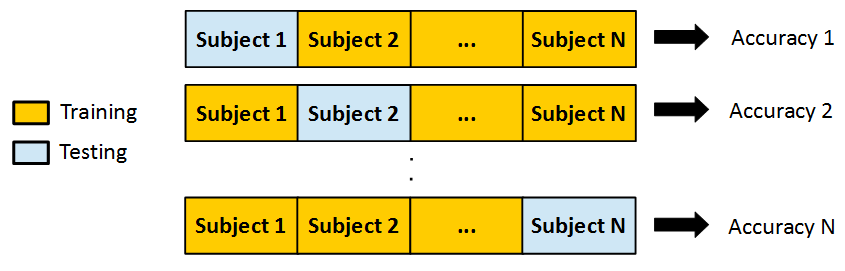
\includegraphics[width=15cm]{Images/LOSOCV.png} 
\caption{ Leave-One-Subjekt-Out-Cross-Validation (LOSOCV): $N$ entspricht der Anzahl der Probanden. Für jeden Split wird ein Testset aus den Daten eines Probanden aufgebaut, während die Daten der anderen Probanden einen Trainingsset bilden. Dieser Vorgang wird für die Daten jedes Probanden durchgeführt. }}
\label{fig:losocv} \end{figure} \vspace{0.5cm}

% 6 Ergebnisse
\newpage
\section{Ergebnisse} \label{ergenisse-sec}
\todo[inline]{Artur}



% Unterkapitel 
\subsubsection{Hand-gefertigte Merkmale} \label{hc-features-subsubsec}







% Unterkapitel 
\subsection{Ergebnisse des Codebook Approach} \label{ergebnisse-codebook-approach-subsec}


{\"A}hnlich wie bei den handgefertigten Merkmalen haben wir die Daten mit einer Normalisierungstechnik vorverarbeitet und dann die Segmentierung verwendet. Die Zeitfensterparameter sind identlisch wie bei der Studie mit den handgefertigten Merkmalen.
F{\"u}r die Klassifizierung haben wir SVM mit Soft-Margins und dem RBF-Kernel benutzt. 
Um die optimalen Parameter des SVM-Klassifikators zu bestimmen (z.B. Soft-Margin $C$ und Kernelparameter $\gamma$), wurde hier wieder die Gitter-Suche angewendet. \\


Die Ergebnisse, die wir mit dem CA mit fester Zuordnung (hard assignment) und $C = 8$, $\gamma = 0,002$ f{\"u}r jeden Probanden erhielten, waren 52\%, 38\% und 38\%, was einem Durchschnitt von 42,67\% entspricht. CA mit Soft-Assignment wurden ebenfalls getestet, lieferte aber schlechtere Ergebnisse als CA mit Hard-Assignment. In diesem speziellen Datensatz schneidet der CA also schlechter ab als die handgefertigten Merkmale.








\subsection{Ergebnisse der Deep Neutral Networks} \label{ergebnisse-dnn}

Die Verwendung von DNNs zur Extraktion von Merkmalen (z.B. Multi-Layer-Perceptron, Convolutional Neural oder Long-Short-Term-Memory Networks) wurden zwar intensiv getestet (siehe \cite{bscschnieber18}), diese Ansätze erreichten aber leider nicht so gute Ergebnisse, wie z.B. die oben vorgestellten Ergebisse der handgefertigten Merkmale. Die beste Performance erreichten LSTM mit einem F1-Score von 47,99\%. \\



% Unterkapitel
\subsection{Analyse der Ergebnisse} \label{analyse-subsec}











% Part 2
%\newpage
%\fancyhf{} \cfoot{\thepage} \rhead{\leftmark \hspace{0.2cm} PART II} % Header Part 2
%\part{Zweiter Prototype}
%\addtocontents{toc}{\protect\mbox{}\protect\hrulefill\par}
%

% 1 Systementwurf
\section{Systementwurf und Konzept} \label{systementwurf-sec}
\todo[inline]{Verantwortlich: Kevin, Jonas}



% Unterkapitel 
\subsection{Anforderungen} \label{anfoderungen-1}

Auf Grundlage der Ziele des Forschungsprojektes ELISE und dem Sichten und Vergleichen von mehr als 30 wissenschaftlichen Veröffentlichungen der letzten 15 Jahre, ergeben sich bestimmte
Anforderungen für den Entwurf eines eigenen Emotionserkennungssystems. Einige wissenschaftliche Veröffentlichungen sind dabei nicht außer Acht zu lassen. Die Foscher von T.
Sharma, S. Bhardwaj und H. B. Maringanti haben in ihrer Veröffentlichung Emotion Estimation
using Physiological Signals versucht, mit Hilfe von GSR, Herzschlagrate,
BVP und der Temperatur Aufschluss über die Emotionen Zorn, Angst, Freude und Traurigkeit
durch Stimulation verschiedener Songs und Videos zu erhalten. Sie erforschten, in
welchen Fällen sich die Körperleitfähigkeit je nach emotionalem Ausdruck unterschiedlich
verhält. H. F. Garcia, A. A. Orozco und M. A. Alvarez versuchten in ihrer Arbeit Dynamic
physiological signal analysis based on Fisher kernels for emotion recognition durch unterschiedliche Klassifizierungsmodelle, die Signale von EEG, EOG, EMG (Elektromyografie),
GSR, Atmung und Temperatur zu analysieren. Dafür wurden 32 Probanden,
die ein 40-minütiges Video mit Musikausschnitten ansahen, aufgezeichnet und ausgewertet.
Durch ein automatisches Regressionsprozess-Modell verbesserten sie dynamische Merkmale
und weitere aufgezeichnete Signale für eine weiterführende Auswertung.
Die Emotionserkennung erfolgte bis vor einigen Jahren in Verbindung mit zusätzlichen Kameras
und Software zur Gesichtsmimik-Erkennung oder Stimmerkennung, nicht jedoch mit
einer reinen Aufnahme von Körpermesswerten. In ELISE sollen insbesondere die lernrelevanten Emotionen Langweile, Frustration, Verwirrung sowie Engagement und Freude erkannt
werden. Die Hardware-Architektur muss auch in diesem Fall wieder das Ziel erfüllen, dass
das Gefühl der Immersion nicht gestört wird. Das heißt, dass das System zur Erkennung von
lernrelevanten Emotionen an möglichst wenigen Stellen am Körper mit zusätzlicher Sensorik
angebracht wird.
Auf Basis der Literaturrecherche, wie in der Bibliographie ausgewiesen, sind folgende Sensoren
zur Aufnahme der lernrelevanten Emotionen ausgewählt worden:

• Gehirnaktivität (EEG)
• Augenbewegung (EOG)
• Blutvolumenpuls (BVP)
• Sauerstoffsättigung im Blut (PPG)
• Hautleitfähigkeit (GSR)
• Körpertemperatur

Da die Sensorwerte zum Mikrocontroller aufgrund ihres räumlichen Abstandes über den
Bus übertragen werden, unterliegen diese Werte den Zeitanforderungen des Datenbusses.
Hier ist zu überprüfen, welches Buskonzept den Zeitanforderungen gewachsen ist.
Um den Aufwand für den Benutzer gering zu halten und die Immersion nicht zu stören,
wird versucht, die Sensorik direkt an der VR-Brille anzubringen. Für die EEG- und
EOG-Sensoren ist dies sowieso notwendig, da diese Messungen lediglich am Kopf stattfinden
können. Zudem soll das Endsystem echtzeitfähig sein, um in der späteren Anwendung
Änderungen und Fluktuationen der Emotionen erkennen zu können und die Schulungen auf
den Lernenden anzupassen. Das Emotionserkennungssystem soll mobil anwendbar sein, da
neuere Versionen der HTC Vive VR-Brille in Zukunft den kabellosen Betrieb unterstützen.
Auch aus diesem Grund ist die Kompaktheit, Energieeffizienz und die Datenübertragung der
einzelnen Sensoren und die Datenübertragung des späteren Gesamtsystems, die ebenfalls
kabellos stattfinden soll, von großem Interesse. Eine mögliche Stelle zur Unterbringung des
Gesamtsystems wäre am Hinterkopf des Probanden, da dort der nötige Platz vorhanden ist
und erforderliche Befestigungsstellen am Kopfband der HTC Vive von Vorteil sind.



% Unterkapitel 
\subsection{Konzept} \label{konzept-1}

Auf Abbildung 1 kann man das Konzept der Architektur erkennen, Dies ist zur besseren Anschauung stark vereinfacht. Hierbei bildet der Mikrocontroller das zentrale Element, welches die einzelnen Sensoren anbindet, steuert und die Messsignale grob zur besseren Auswertung verarbeitet. Zur besseren und möglichst in Echtzeit stattfindeten Verarbeitung werden die Daten an einen externen Rechner weitergeleitet. In der Abbildung findet diese Weiterleitung Drahtlos mittels Bluetooth statt. Es wurden in den verschiedenen Prototypen für diese Zwecke sowohl Bluetooth als auch WLAN verwendet. Für die Teilsysteme EEG und EOG wurden schon einfache Physische Filter auf den Leiterplatten vorgesehen, welche die analogen Signale vorberarbeiten, bevor dies von einem AD-Wandler digitalisiert werden. Da die Elektroden für die EEG und EOG Messung nur am Kopf angebracht werden können, empfiehlt es sich die übrigen festgelegten Werte ebenfalls am Kopf zu messen. Um die Messung für möglichst viele Personen mit unterschiedlichen Kopfformen zu ermöglichen wurde zuerst ein elastisches Kopfband und später eine flexible Maske verwendet. All dies wurde für eine spätere Verwendung mit (unter) einer VR-Brille designet. 





% Unterkapitel
\subsection{Hardwareauswahl} \label{hardwareauswahl-1}

Bei der Wahl der richtigen Hardware zur Aufnahme, Verarbeitung und Weiterleitung von
biomedizinischen Signalen, sind die reinen Hardwarekosten von untergeordneter Bedeutung.
Jedoch sollte das Budget für das spätere Gesamtsystem einen gewissen Rahmen nicht überschreiten,
um auch die aufkommenden Endkosten in Verbindung mit einer VR-Brille und der
benötigten Hardware zur Darstellung der Lerninhalte in einem gewissen Rahmen zu halten.
Die Bandbreite der angebotenen Systeme von unterschiedlichen Mikrocontrollern ist dabei
sehr groß. Zu Beginn einer geeigneten Neubeschaffung sollten, wie bei jedem IT-Projekt, die
zuvor genannten Anforderungen an das System betrachtet werden und daraus Auswahlkriterien
für die geeignete Hardware gewählt werden.

% Unterkapitel 
\input{Part-1/1-Systementwurf/3-Hardwareauswahl/1-auswahlkriterien}

% Unterkapitel 
\input{Part-1/1-Systementwurf/3-Hardwareauswahl/2-festlegung-hardware}



% Unterkapitel
\subsection{Hardwarearchitektur} \label{hardwarearchitektur-subsec}



% Unterkapitel
\input{Part-4/1-Systementwurf/4-Hardwarearchitektur/1-gsr}

% Unterkapitel
\input{Part-4/1-Systementwurf/4-Hardwarearchitektur/2-temperatur}

% Unterkapitel 
\input{Part-4/1-Systementwurf/4-Hardwarearchitektur/3-pulsoximeter}

% Unterkapitel 
\input{Part-4/1-Systementwurf/4-Hardwarearchitektur/4-eeg}

% Unterkapitel 
\input{Part-4/1-Systementwurf/4-Hardwarearchitektur/5-eog}

% Unterkapitel
\input{Part-4/1-Systementwurf/4-Hardwarearchitektur/6-datenuebertragung}



% Unterkapitel 
\subsection{Programmierung} \label{programmierung-subsec}

Die Programmierung des dritten Prototypen basiert im wesentlichen auf der des zweiten Protoypen, da sich in Bezug auf die Hardware nur die GSR-Schaltung geändert hat. Wie auch bei vorherigen Prototypen erfolgte die Programmierung mit Hilfe der Arduino Plattform und der durch die Hersteller schon zur Verfügung gestellten Bibliotheken.





% Unterkapitel 
\subsection{Aufnahme der {\"u}bertragenen Daten} \label{aufnahme-daten-subsec}

Beim dritten Prototypen wurden die Daten wieder drahtlos übertragen. Im Gegensatz zum ersten Prototypen kam hier aber nicht mehr ein Bluetooth-Modul zum Einsatz, sondern das im ESP32 integrierte WLAN-Modul. In den mit diesem Prototypen durchgeführten Messungen wurden die Daten mittels WireShark aufgenommen und abgespeichert. Diese Daten wurden später zur Datenanalyse in eine CSV-Datei umgewandelt. Zur Übertragung wurde das zuvor schon beschriebene UDP-Protokoll  verwendet. An dieser Stelle sei noch einmal Erwähnt, das alle Daten mit einer Abtastrate von 250 Samples pro Sekunde gemessen wurden. Die einzige Ausnahme hier ist die Temperatur, die lediglich mit einer Rate von 3,3 Samples pro Sekunde gemessen wurde. 




% 2 Realisierung
\newpage
\section{Realisierung} \label{realisierung-sec}


Für den ersten Versuch mit Testpersonen wurden die Experimente zur Emotionsinduktion zu einem Gesamtexperiment verbunden. Dabei wurde darauf geachtet einen möglichst automatisierten Testablauf zu erreichen, so dass die Testperson möglichst unbeeinflusst von äußeren Reizen oder den Aktionen des Testleiters bleibt. Dazu wurde eine automatisierte Webanwendung programmiert, die der Versuchsperson alle Anweisungen und Experimente präsentiert (siehe Abbildung \ref{fig:screen_soft1}). Der Versuchsleiter wiederum kann durch eine, ebenfalls webbasierte, Kontrollkonsole Einfluss auf das Experiment nehmen, in dem er zum Beispiel den Ablauf stoppen oder Schritte überspringen kann (siehe Abbildung \ref{fig:screen_soft1}).\\

Die Ablaufkontrolle erfolgt über den Flask Webserver, der die Website darstellt. Zur Steurung können einfach URLs auf dem Server mittels einer GET bzw. POST Anfrage aufgerufen werden und so Steuerbefehle übermittelt werden. \\

Die Bilder, die dem Probanden angezeigt werden, wie auch die Spiele, die er spielen soll, sind nahtlos in die Website eingebettet. Dies ist möglich, dadurch, dass es sich zum einen um eine Javascript Anwendung und zum anderen um eine Flash Anwendung handelt. Die Flash Anwendung wurde zur einfacheren Handhabung so präpariert, dass das Menü entfernt wurde und das Spiel direkt mit dem ersten Level beim Laden startet. \\

\begin{figure}[h]
    \centering
\begin{minipage}[t]{0.9\textwidth}
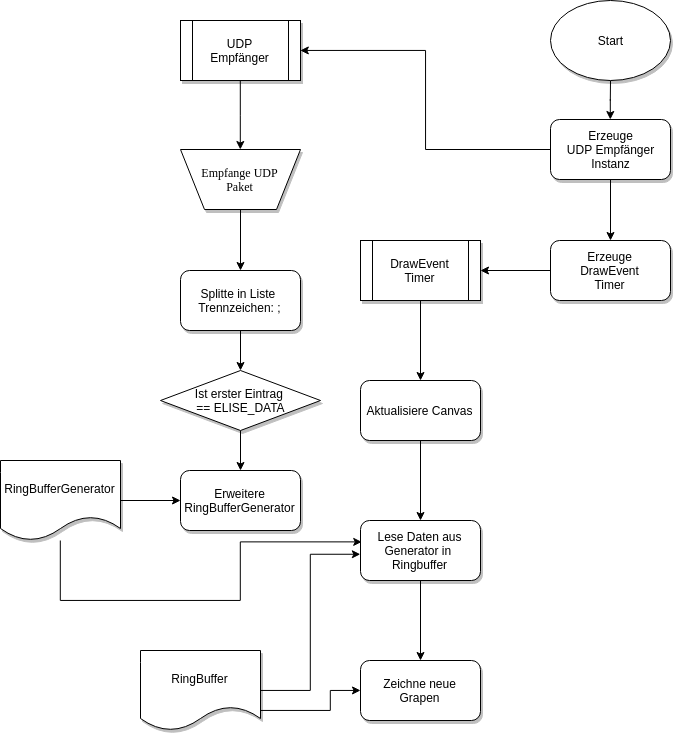
\includegraphics[width=\textwidth]{Images/ablauf_anzeige.png}
\end{minipage}
    \caption{Screenshot der Supervisor Ansicht}
    \label{fig:screen_soft1}
\end{figure}





% 3 Emotionsinduktion
\newpage
\section{Emotionsinduktion} \label{emotionsinduktion-sec}
\todo[inline]{Verantwortlich: Minas}


% Unterkapitel
\subsection{Ablauf} \label{ablauf-1}


\todo[inline]{Verantwortlich: Minas}


Der Ablauf der Emotionsinduktion lief wie folgt ab:

\begin{itemize}
\item[1.] Gl{\"u}ck (PowerPoint) $\rightarrow$ Kapitel 7.3.1
\item[2.] Langeweile (Video) $\rightarrow$ Kapitel 7.3.2
\item[3.] Frustration (Flashgame) $\rightarrow$ Kapitel 7.3.3
\item[4.] Langeweile (Spiel im Browser) $\rightarrow$ Kapitel 7.3.2
\end{itemize}

Nach jedem Szenario folgte ein sich automatisch {\"o}ffnender Fragebogen zum Szenario. 
Der Wechsel zwischen den Szenarien musste manuell statt finden.

% Unterkapitel 
\subsection{Fragebogen} \label{fragebogen-4}


\todo[inline]{Verantwortlich: Boris\\
- add picture of VR questionare (both dominat emotions and circumplex)}

F{\"u}r dieses Prototyp wurden zwei Arten von Frageb{\"o}gen benutzt. 
Der erste Typ ist sehr {\"a}hnlich mit dem von der zweite Prototyp. Es enth{\"a}lt in dem informativen Teil einen Text, wo es beschrieben wird, wie der Fragebogen ausgef{\"u}llt werden soll. Der andere Teil besteht aus vier Dropdown-Boxen von dreizehn Optionen, die zw{\"o}lf verschiedene Emotionen und einen als null oder neutral geltenden Zustand enthalten. Jede Dropdown-Box entspricht ein Viertelzeit der Szenario. Es soll zwischen die Optionen jeder Dropdown-Box gew{\"a}hlt werden, welche Emotion es am st{\"a}rksten empfindet wird, je nachdem, wann man es f{\"u}hlte, d.h. ob es das erste, zweite, dritte oder letzte Quartal der Zeit des Videos war, um die Emotion zu bew{\"a}ltigen. Unten gibt es ein Button wo man dr{\"u}cken kann, wenn man fertig ist. Allerdings hat man auch die M{\"o}glichkeit seine Wahl zu {\"a}ndern, auch wenn man sich schon im n{\"a}chsten Schritt befindet, indem man in diesem n{\"a}chsten Schritt auf den Zur{\"u}ck-Button dr{\"u}ckt und die gew{\"u}nschten {\"a}nderungen vornimmt. Hierf{\"u}r wird ein Widget Blueprint erstellt, die vier Dropdown-Boxen mit dem gew{\"u}nschten Anzahl an Optionen hinzugef{\"u}gt und die Labels von der unterschiedlichen Optionen der Dropdown-Boxen definiert. Ein Button ``next'' wird auch erstellt um zum n{\"a}chsten Fragebogen zu navigieren. Es wird auch eine zwischen Speicherungsfunktion in ein anderes Skript definiert, die hier aufgerufen wird, um die {\"a}nderung auch nach das dr{\"u}cken von dem ``next'' Button zu Speichern. Dabei wird vier Variablen definiert und die Werte von der gew{\"a}hlten Optionen werden ihnen zugewiesen. \\



\begin{figure}[H] \centering
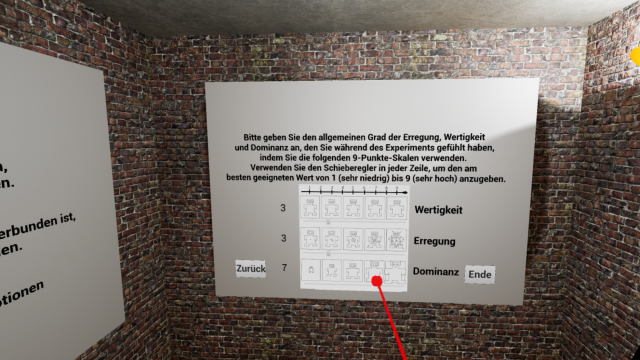
\includegraphics[width=\textwidth]{Images/Fragebogen_3.png} 
\caption{ Bild des Fragebogen-Teils, entsprechend dem circumplex-Modell. } 
\label{fig:fragenbogen4} \end{figure}



Der zweite Typ {\"a}hnelt dem ber{\"u}hmten Modell von James Russels ``circumplex'' \cite{russel_1980}. Es ist ein klassisches Modell mit einer kreisf{\"o}rmigen Struktur, die auf zwei senkrechten Diagonalen ruht. Die vertikale Achse, die die Erregung darstellt, und die horizontale Achse, die die Valenz darstellt. Das Zentrum des Kreises stellt eine neutrale Valenz und ein mittleres Erregungsniveau dar. Andere Emotionen werden auf jeder Ebene des Kreises dargestellt.  Hier wird ein weniger bekanntes Modell verwendet, das ``Self Assessment Manikin'' (SAM). Es besteht aus drei Reihen mit je f{\"u}nf Piktogrammen. Diese Piktogramme stellen den Zustand eines Gesichts nach verschiedenen Arten von Emotionen dar. So repr{\"a}sentiert der erste Bereich die Wertigkeit, der zweite die Erregung und der dritte die Dominanz. Eine Erkl{\"a}rung zu jedem dieser Begriffe ist ebenfalls neben dem Fragebogen enthalten, um die Testpersonen {\"u}ber diese W{\"o}rter aufzukl{\"a}ren.  Bei jeder Avatar und in der Mitte jeder der beiden Avatar befindet sich ein Checkbox.  So muss man f{\"u}r jede Zeile das Checkbox ausw{\"a}hlen, das ihrem emotionalen Zustand am besten entspricht. Man kann nur ein Checkbox pro Zeile markieren und man hat auch die M{\"o}glichkeit wie bei dem ersten Model seine Wahl zu {\"a}ndern. Es kann einfach mit Branch-Bedingungen realisieren werden.  Diese werden auch in eine Widget Blueprint wie f{\"u}r das erste Modell gemacht. Es gibt auch wieder die zwischen Speicherungsfunktion und das Button ``next''. Was neues hier kommt ist das Button ``back'' um wieder zum ersten Fragebogen zu navigieren. 



\begin{figure}[H] \centering
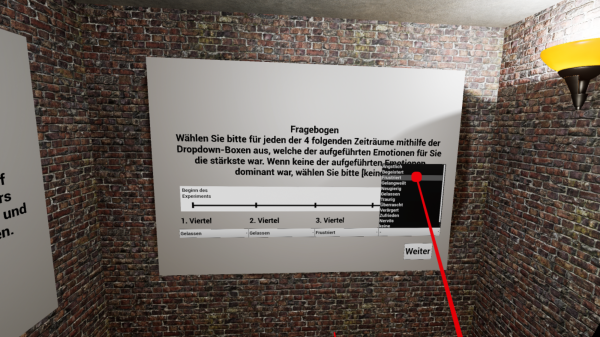
\includegraphics[width=\textwidth]{Images/Fragebogen_1.png} 
\caption{ Bild des Fragebogen-Teils, wo die dominierenden Emotionen abgefragt werden. } 
\label{fig:fragenbogen1} \end{figure}

% Unterkapitel 
\subsection{Szenarien} \label{szenarien-subsec}

\todo[inline]{Verantwortlich: Meryem}

% Unterkapitel 
\input{Part-1/3-Emotionsinduktion/3-Szenarien/1-glueck}

% Unterkapitel 
\input{Part-1/3-Emotionsinduktion/3-Szenarien/2-langeweile}

% Unterkapitel 
\input{Part-1/3-Emotionsinduktion/3-Szenarien/3-frust}


% 4 Messreihe
\newpage
\section{Messreihe} \label{messreihe-sec}
\todo[inline]{Kevin, Artur}




% 5 Mustererkennung
\newpage
\section{Mustererkennung} \label{mustererkennung-sec}

\todo[inline,color=green!40]{Verantwortlich: Artur\\
- RfP}

In diesem Kapitel werden alle Schritte entlang der ERC (vgl. Kapitel \ref{emotion-recogniton-chain}) konkretisiert und es wird detailreich beschrieben, wie wir vorgegangen sind. \\


% 1 Datenerfassung
\subsection{Datenerfassung} \label{datenerfassung-1}


In Kapitel \ref{messreihe-1-sec} wurde das verwendete Datenset bereits detailiert beschrieben, sodass hier darauf verzichtet wird. \\

% 2 Vorverarbeitung
\subsection{Vorverarbeitung} \label{vorverarbeitung-1}

Wie bereits in Kapitel \ref{vorverarbeitung-0} beschrieben, ist das Ziel der Vorverarbeitung die ”Verbesserung” der Daten f{\"u}r die nachfolgenden Schritte der ERC.
Im Rahmen des ELISE Projektes wurden Normalisierungstechniken auf dem gesamten Datensatz angewendet. 
Wir haben insbesondere die Standardnormalisierung verwendet, welche den Mittelwert der Daten auf Null setzt und die Einheitsvarianz ergibt \cite{grus15}. 
Die Formel f{\"u}r die Standardnormierung lautet:
\begin{equation} 
\Large{ {x'={\frac {x-{\overline {x}}}{\sigma }}} } 
\label{equ:norm} \end{equation} %\vspace{0.5cm}

wobei $ x $ ein Datenpunkt eines Sensorkanales, $ \overline{x} $ ist der Durchschnitt der Gesamtheit f{\"u}r diesen Sensorkanal und $ \sigma $ ist die entsprechende Standardabweichung. \\

% 3 Segmentation
\subsubsection{Segmentation} \label{segmentation-0}

Ziel dieses Schrittes ist es, Teile von Daten zu identifizieren, welche wichtige Informationen über die zu erkennenden Emotionen enthalten. 
Dies geschieht durch Filtern der Daten und Ausschließen von Segmenten, die für das Klassifizierungsproblem nicht relevant sind.
Zusätzlich wird die zu verarbeitende Datenmenge reduziert, indem Segmente eines Zeitfensters fester Größe aus den Daten extrahiert werden.
Diese Vorgeheisweise ist heute in der Praxis besonders wichtig, da sonst hardwarebedingte Einschränkungen die zu verarbeitende Datenmenge begrenzen könnten. \\

% 4 Merkmalsextraktion
\subsection{Merkmalsextraktion} \label{merkmalsextraftion-1}

Wie bereits in Kapitel \ref{merkmalsextraktion-subsubsec} beschrieben, ist das Ziel der Merkmalsextraktion Charakteristiken und Merkmale in den Daten zu finden, die für das
Klassifizierungsproblem von möglichst hoher Relevanz sind. Im Rahmen des ELISE Projektes haben wir verschiedene Vorgehensweisen angewendet. Im den folgenden Unterkapiteln werden diese vorgestellt. \\



% Unterkapitel 
\subsubsection{Handgefertigte Merkmale} \label{hc-features-1}
Der handgefertigten Merkmal Ansatz (enlg. "hand-crafted features approach") besteht in der Berechnung relativ einfacher Merkmale von denen vermudetet wird, dass sie für das Klassifizierungsproblem der Eingangssignale relevant sein können. Diese Vorgehensweise hat den Vorteil des einfachen Aufbaus als auch der relativ geringen benötigten Rechenleistung, wobei potentiell gute Klassifizierungsergebnisse erwarten werden. \\


Obwohl frühere Forschungsarbeiten schon handgefertigte Merkmale zur Emotionserkennung unter mithilfe physiologischer Signale getestet haben (vgl. \cite{martinez_ieee_2013}), wurde dieser Ansatz noch nie für die Erkennung dieser spezifischen Emotionen unter Verwendung dieser Kombination von Sensoren getestet.
Zusätzlich haben wir zuerst handgefertigte Merkmale getestet, um ein Basisergebnis zu liefern, mit der die Ergebnissen der anderen Ansätze vergleichen werden können.
Handgefertigte Merkmale sind in der Regel entweder einfache statistische Werte, Fourier-basierte oder selbstentwickelte Merkmale sein, die aufgrund von Vorkenntnissen der Daten verwendet werden. 
Diese Arbeit wurden statistische, Fourier-basierte und selbstentwickelte Merkmale getestet. \\

\textbf{Statistische Merkmale \\}
Die Tabelle \ref{tab:statistische} fasst die elf verschiedenen und in der Studie verwendeten statistischen Merkmale zusammen. Wir bezeichnen $\mathbf{x} = (x_1, x_2, ...., x_T) $ als Vektor, der die in einem Datenzeitfenster der Länge $T$ enthaltenen Sensorwerte für einen Sensorkanal darstellt. 


\begin{table}[h]
\begin{tabular}{| l | p{12.5cm} |}
\hline
    \textbf{Merkmalname}     &  \textbf{Definition}  \\ \hline
    
    Durchschnitt         & \vspace{0.01cm}
    $ mean(\mathbf{x}) =$ \Large{$\frac{1}{T} \sum_{k=1}^T (x_k) $} \\[0.5cm] \hline 
    
    Standard-Abweichung        & \vspace{0.01cm}
    $ \sigma(\mathbf{x}) =$ \Large{$ \sqrt{ \frac{1}{T} \sum_{k=1}^{T}{(x_k - \mu)^{2}} } $ } \\[0.5cm] \hline
    
    Maximum                   & \vspace{0.01cm}
    $ max(\mathbf{x}) = \max(x_{1},x_{2},\dots ,x_{T}) $
    \\[0.5cm] \hline
    
    Minimum                   & \vspace{0.01cm}
    $ min(\mathbf{x}) = \min(x_{1},x_{2},\dots ,x_{T}) $
    \\[0.5cm] \hline
    
    Amplitude                 & \vspace{0.01cm}
    $ A(\mathbf{x}) = max(\mathbf{x}) - min(\mathbf{x}) $ 
    \\[0.5cm] \hline
    
    25/50/75\% Perzentil      & Wert einer Menge, unter dem 25/50/75\% der Werte aus der Menge fallen. \\ \hline
    
    Interquartiler Bereich    & Differenz zwischen dem 75. und 25. Perzentil.
    \\ \hline
     
    Schräge                   & \vspace{0.01cm}
    $ \gamma _{1}(\mathbf{x}) = \operatorname{E}$ \Large{$\left[\left({\frac {X-\mu }{\sigma }}\right)^{3}\right]$ \normalsize{$=$} ${\frac {\mu _{3}}{\sigma ^{3}}}$ \normalsize{$=$} ${\frac {\operatorname {E} \left[(X-\mu )^{3}\right]}{ (\operatorname {E} \left[(X-\mu )^{2}\right])^{3/2}}}$ \normalsize{$=$} ${\frac {\kappa _{3}}{\kappa _{2}^{3/2}}} $} \vspace{0.2cm}
    \\[0.3cm] \hline
     
    Kurtosis                  & \vspace{0.01cm}
    $ \operatorname {Kurt}[\mathbf{x}] = \operatorname{E} $ \Large{$\left[\left({\frac {X-\mu }{\sigma }}\right)^{4}\right]$ \normalsize{$=$} ${\frac {\mu _{4}}{\sigma ^{4}}}$ \normalsize{$=$} ${\frac {\operatorname {E} [(X-\mu )^{4}]}{(\operatorname {E} [(X-\mu )^{2}])^{2}}} $} \vspace{0.2cm}
    \\[0.3cm] \hline
\end{tabular} 
\caption{Statistische Merkmale, die im Rahmen des ELISE-Projektes verwendet wurden. } \label{tab:statistische}
\end{table} 


\textbf{Fourier-basierte Merkmale \\}
\todo[inline]{Artur: \\
- Muss ich noch schreiben $\rightarrow$ Warten auf Julian's Antwort. \\}


\textbf{Selbstentwickelte Merkmale \\}
Es wurden zwei eigene Merkmale definiert: Nulldurchgang (engl. "zero crossing") und Anzahl der Spitzen (engl. "number of peaks"). Im Folgendem werden diese beiden Merkmale detailiert beschrieben. \\

Das Nulldurchgang-Merkmal zählt die Häufigkeit, mit der das Signal eines Sensorkanals in einem Zeitfenster die Nulllinie überschreitet.
Alle Sensorsignale wurden durch Normierung verarbeitet (vgl. Kapitel xxx) und damit wurden alle Mittelwerte auf Null zentriert.
Um zu vermeiden, dass Rauschen entlang der Nulllinie in dem Merkmal gezählt wird, wird nur ein Nulldurchgang in einer bestimmten Zeitspanne gezählt. \\


Das Spitzenzähler-Merkmal bestimmt die Anzahl von loklanen Hochpunkten im Zeitsignal.
Alle lokalen Maximen sind durch einen Onset (Startpunkt), eine Spitze und einen Offset (Endpunkt) gekennzeichnet (vgl. Abbildung \ref{fig:peaks}). 
Jedes Vorkommen einer Onset/Offset-Paarung wird hierbei als Spitze gezählt.
Onsets, Spitzen und Offsets werden durch die folgenden Operationen identifiziert \cite{BSc_Gouverneu}:

\begin{itemize} %[noitemsep]
  \item Ein Onset wird bestimmt, wenn der Wert des Signals an diesem Punkt nicht negativ ist und die Differenz zwischen ihm und dem nächsten größer als ein vordefinierter Schwellenwert (engl. "threshold") ist.

  \item Ein Offset wird bestimmt, wenn der Wert des Signals kleiner als der Wert des zuletzt gesetzten Onsets ist.

  \item Das lokale Maximum zwischen einem Onset und Offset wird als Spitze bezeichnet.
\end{itemize} \vspace{0.2cm}


\begin{figure}[h] \centering{
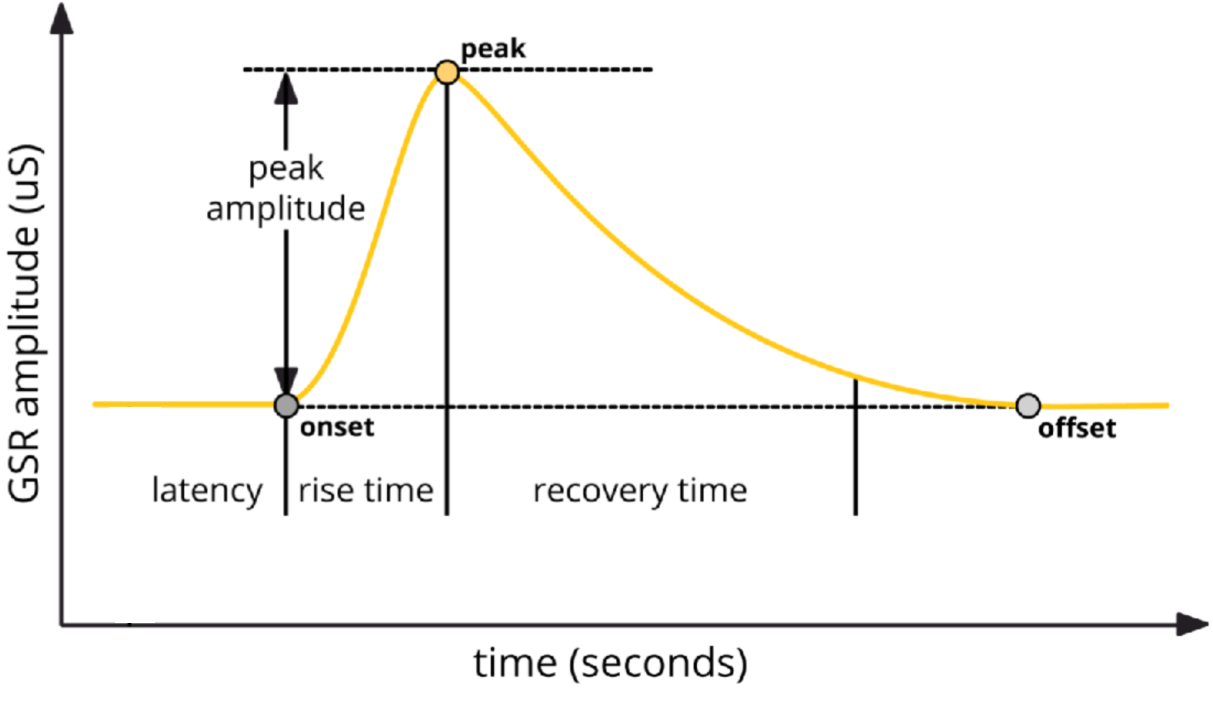
\includegraphics[width=11cm]{Images/peaks.png}}
\caption{ Spitzenzähler: Onset (Startpunkt), Spitze und Offset (Endpunkt). Jedes Paar von Onset/Offset erhöht die Anzahl der Spitzen um eins.} 
\label{fig:peaks} \end{figure} \vspace{0.5cm}


Jedes handgefertigte Merkmal wird auf einem Zeitfenster von Daten für jeden Sensorkanal unabhängig voneinander angewendet. 
Jedes Zeitfenster ist daher 117 Merkmalen zugeordnet (9 Sensorkanäle multipliziert mit 13 Merkmalen). \\





% Unterkapitel 
\subsubsection{Codebook Approach} \label{ca-1}


Die bisherige Methodik mit handgefertigten Merkmalen ist klassisch für den überwachten Lernansatz. 
Es existieren aber auch einige Nachteile. 
Das Hauptproblem besteht darin, dass nicht sichergestellt werden kann, dass die gewählten Merkmale die besten Klassifizierungsergebnisse erzielen. Damit besteht immer die Gefahr, dass möglicherweise andere Merkmalen bessere Ergebnisse liefern würden, diese handgefertigten Merkmale aber die  nicht gefunden wurden. Dieses Risiko besteht insbesondere bei der physiologischen Signalverarbeitung zur Emotionserkennung, wo die Struktur der Daten noch recht unbekannt und allgemein komplex ist. 
Eine weitere Schwierigkeit besteht darin, relevante selbstentwickelte Features ohne Expertenwissen über die Daten zu finden.
Darüber hinaus wurden noch keine gut funktionierenden State-of-the-Art handgefertigten Merkmale identifiziert.
Aus diesen Gründen ist es interessant halbautomatische und unüberwachter Ansätze der Merkmalsextraktion zu verwenden und zu testen. \\


K. Shirahama et al. \cite{kimiaki_codebook_approach_2016} schlugen eine unüberwachte Merkmalsextraktionsmethode namens Codebook Approach (CA) vor, um Merkmale aus 1D-Zeitreihensignalen zu erzeugen.
Der CA hat den Vorteil, dass formbasierte Merkmale gefunden werden können, die für das Problem der Emotionserkennung relevant sind, aber weder offensichtlich noch leicht als Mensch zu interpretieren sind. 
Der CA besteht aus drei Schritten, die in den folgenden Abschnitten erläutert werden: Codebuchkonstruktion (engl. "codebook construction"), Codewortzuordnung (engl. "codeword assignment") und der anschließenden Klassifizierung. \\


\textbf{Codebuchkonstruktion \\}
Ziel dieses Schrittes ist es, Teilsequenzen (sogenannte "Codewörter") zu bestimmen, die für die 1D-Eingangssensorik charakteristisch sind. 
Dies wird erreicht, indem Zeitfenster aus dem ursprünglichen Datensatz für jeden Sensorkanal unabhängig voneinander nach dem im Kapitel \ref{segmenation-1} definierten Segmentierungsansatz extrahiert werden.
Aus jedem so erhaltenen Zeitfenster der Größe $T$ werden kleinere Segmente der Größe $\alpha$ unterteilt.
Ein Clustering-Algorithmus wird dann auf die Menge der Segmente $\alpha$ angewendet, um Clusterzentren zu finden.
Nach der Konvergenz werden die Clusterzentren als Codewörter betrachtet und zum Aufbau einer Sammlung von Codewörtern mit dem Namen ``Codebuch'' verwendet, wie in Abbildung \ref{fig:ca_construction} aus \cite{kimiaki_codebook_approach_2016} dargestellt. 
Die Anzahl der Codewörter (d.h. die Größe des Codebuchs oder die Anzahl der Cluster) ist ein Hyperparameter des Verfahrens. Im Rahmen dieser Arbeit wurde ein k-means Clustering-Algorithmus verwendet, um die Codewörter auf den ELISE-Daten zu erhalten. \\



% 5 Klassifikation
\subsection{Klassifikation} \label{klassifikation-1}

Wie bereits in Kapitel \ref{grundlagen-klassifikation-0} beschrieben ist das Ziel der Klassifizierung ein Klassifizierungsmodell zu trainieren, das in der Lage ist, Objekte in den Daten in die entsprechende Klasse zuzuordnen. Die Klassen entsprechen hierbei den Emotionen, die erkannt werden sollen: Glück, Langeweile, Frustation und andere (d.h. alle Emotionen, die nicht Glück, Langeweile oder Furstation entsprechen). \\

Als erstes wird der Datensatz in ein Trainigs- und Testset  aufgeteilt. 
Es gibt keine festgelegten Regeln über die Proportionen der Sets. 
Im Allgemeinen wird das Trainingsset aber größer als das Testset gewählt.
Da die Leistungen des Klassifikators jedoch stark von der gewählten Aufteilung abhängen, ist es wichtig, sicherzustellen, dass dieser Schritt richtig durchgeführt wird.
Bei einem Datensatz mit mehreren Probanden empfiehlt sich für die Aufteilung zwischen Trainings- und Testsets die Durchführung einer Leave-One-Subjekt-Out-Cross-Validierung (LOSOCV).
Die Idee besteht darin, $N$ verschiedene Aufteilungen des Datensatzes vorzunehmen, wobei $N$ die Anzahl der Personen ist, die Daten für den Datensatz bereitgestellt haben. 
Für jeden dieser Splits wird der Testset aus den Daten eines Probanden aufgebaut, während die Daten der anderen Probanden das Trainingsset bilden. 
Anschließend wird ein Klassifizierer erstellt und ausgewertet. Dies wird für alle Probanden wiederholt, d.h. $N$ mal.
Die so erhaltenen $N$-Bewertungskennzahlen (eine pro Proband) können dann gemittelt werden, um eine Gesamtbewertung des Modells zu erhalten.
Es ist wichtig zu beachten, dass der LOSOCV-Ansatz bei einer hohen Anzahl von Probanden sehr rechenintensiv sein kann. \\

\begin{figure}[h] \centering{
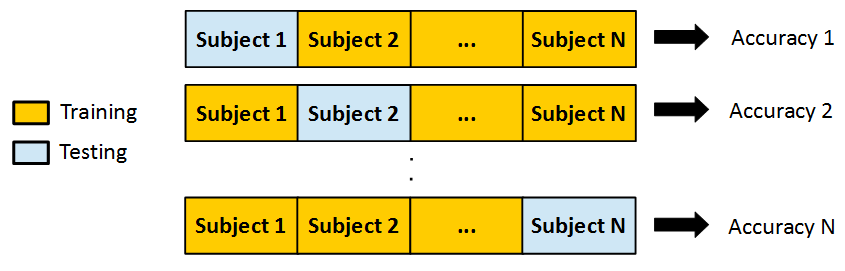
\includegraphics[width=15cm]{Images/LOSOCV.png} 
\caption{ Leave-One-Subjekt-Out-Cross-Validation (LOSOCV): $N$ entspricht der Anzahl der Probanden. Für jeden Split wird ein Testset aus den Daten eines Probanden aufgebaut, während die Daten der anderen Probanden einen Trainingsset bilden. Dieser Vorgang wird für die Daten jedes Probanden durchgeführt. }}
\label{fig:losocv} \end{figure} \vspace{0.5cm}

% 6 Ergebnisse
\newpage
\section{Ergebnisse} \label{ergenisse-sec}
\todo[inline]{Artur}



% Unterkapitel 
\subsubsection{Hand-gefertigte Merkmale} \label{hc-features-subsubsec}







% Unterkapitel 
\subsection{Ergebnisse des Codebook Approach} \label{ergebnisse-codebook-approach-subsec}


{\"A}hnlich wie bei den handgefertigten Merkmalen haben wir die Daten mit einer Normalisierungstechnik vorverarbeitet und dann die Segmentierung verwendet. Die Zeitfensterparameter sind identlisch wie bei der Studie mit den handgefertigten Merkmalen.
F{\"u}r die Klassifizierung haben wir SVM mit Soft-Margins und dem RBF-Kernel benutzt. 
Um die optimalen Parameter des SVM-Klassifikators zu bestimmen (z.B. Soft-Margin $C$ und Kernelparameter $\gamma$), wurde hier wieder die Gitter-Suche angewendet. \\


Die Ergebnisse, die wir mit dem CA mit fester Zuordnung (hard assignment) und $C = 8$, $\gamma = 0,002$ f{\"u}r jeden Probanden erhielten, waren 52\%, 38\% und 38\%, was einem Durchschnitt von 42,67\% entspricht. CA mit Soft-Assignment wurden ebenfalls getestet, lieferte aber schlechtere Ergebnisse als CA mit Hard-Assignment. In diesem speziellen Datensatz schneidet der CA also schlechter ab als die handgefertigten Merkmale.








\subsection{Ergebnisse der Deep Neutral Networks} \label{ergebnisse-dnn}

Die Verwendung von DNNs zur Extraktion von Merkmalen (z.B. Multi-Layer-Perceptron, Convolutional Neural oder Long-Short-Term-Memory Networks) wurden zwar intensiv getestet (siehe \cite{bscschnieber18}), diese Ansätze erreichten aber leider nicht so gute Ergebnisse, wie z.B. die oben vorgestellten Ergebisse der handgefertigten Merkmale. Die beste Performance erreichten LSTM mit einem F1-Score von 47,99\%. \\



% Unterkapitel
\subsection{Analyse der Ergebnisse} \label{analyse-subsec}











% Part 3
\newpage
\fancyhf{} \cfoot{\thepage} \rhead{\leftmark \hspace{0.2cm} PART II} % Header Part 3
\part{Zweiter Prototype}
\addtocontents{toc}{\protect\mbox{}\protect\hrulefill\par}


% 1 Systementwurf
\section{Systementwurf und Konzept} \label{systementwurf-sec}
\todo[inline]{Verantwortlich: Kevin, Jonas}



% Unterkapitel 
\subsection{Anforderungen} \label{anfoderungen-1}

Auf Grundlage der Ziele des Forschungsprojektes ELISE und dem Sichten und Vergleichen von mehr als 30 wissenschaftlichen Veröffentlichungen der letzten 15 Jahre, ergeben sich bestimmte
Anforderungen für den Entwurf eines eigenen Emotionserkennungssystems. Einige wissenschaftliche Veröffentlichungen sind dabei nicht außer Acht zu lassen. Die Foscher von T.
Sharma, S. Bhardwaj und H. B. Maringanti haben in ihrer Veröffentlichung Emotion Estimation
using Physiological Signals versucht, mit Hilfe von GSR, Herzschlagrate,
BVP und der Temperatur Aufschluss über die Emotionen Zorn, Angst, Freude und Traurigkeit
durch Stimulation verschiedener Songs und Videos zu erhalten. Sie erforschten, in
welchen Fällen sich die Körperleitfähigkeit je nach emotionalem Ausdruck unterschiedlich
verhält. H. F. Garcia, A. A. Orozco und M. A. Alvarez versuchten in ihrer Arbeit Dynamic
physiological signal analysis based on Fisher kernels for emotion recognition durch unterschiedliche Klassifizierungsmodelle, die Signale von EEG, EOG, EMG (Elektromyografie),
GSR, Atmung und Temperatur zu analysieren. Dafür wurden 32 Probanden,
die ein 40-minütiges Video mit Musikausschnitten ansahen, aufgezeichnet und ausgewertet.
Durch ein automatisches Regressionsprozess-Modell verbesserten sie dynamische Merkmale
und weitere aufgezeichnete Signale für eine weiterführende Auswertung.
Die Emotionserkennung erfolgte bis vor einigen Jahren in Verbindung mit zusätzlichen Kameras
und Software zur Gesichtsmimik-Erkennung oder Stimmerkennung, nicht jedoch mit
einer reinen Aufnahme von Körpermesswerten. In ELISE sollen insbesondere die lernrelevanten Emotionen Langweile, Frustration, Verwirrung sowie Engagement und Freude erkannt
werden. Die Hardware-Architektur muss auch in diesem Fall wieder das Ziel erfüllen, dass
das Gefühl der Immersion nicht gestört wird. Das heißt, dass das System zur Erkennung von
lernrelevanten Emotionen an möglichst wenigen Stellen am Körper mit zusätzlicher Sensorik
angebracht wird.
Auf Basis der Literaturrecherche, wie in der Bibliographie ausgewiesen, sind folgende Sensoren
zur Aufnahme der lernrelevanten Emotionen ausgewählt worden:

• Gehirnaktivität (EEG)
• Augenbewegung (EOG)
• Blutvolumenpuls (BVP)
• Sauerstoffsättigung im Blut (PPG)
• Hautleitfähigkeit (GSR)
• Körpertemperatur

Da die Sensorwerte zum Mikrocontroller aufgrund ihres räumlichen Abstandes über den
Bus übertragen werden, unterliegen diese Werte den Zeitanforderungen des Datenbusses.
Hier ist zu überprüfen, welches Buskonzept den Zeitanforderungen gewachsen ist.
Um den Aufwand für den Benutzer gering zu halten und die Immersion nicht zu stören,
wird versucht, die Sensorik direkt an der VR-Brille anzubringen. Für die EEG- und
EOG-Sensoren ist dies sowieso notwendig, da diese Messungen lediglich am Kopf stattfinden
können. Zudem soll das Endsystem echtzeitfähig sein, um in der späteren Anwendung
Änderungen und Fluktuationen der Emotionen erkennen zu können und die Schulungen auf
den Lernenden anzupassen. Das Emotionserkennungssystem soll mobil anwendbar sein, da
neuere Versionen der HTC Vive VR-Brille in Zukunft den kabellosen Betrieb unterstützen.
Auch aus diesem Grund ist die Kompaktheit, Energieeffizienz und die Datenübertragung der
einzelnen Sensoren und die Datenübertragung des späteren Gesamtsystems, die ebenfalls
kabellos stattfinden soll, von großem Interesse. Eine mögliche Stelle zur Unterbringung des
Gesamtsystems wäre am Hinterkopf des Probanden, da dort der nötige Platz vorhanden ist
und erforderliche Befestigungsstellen am Kopfband der HTC Vive von Vorteil sind.



% Unterkapitel 
\subsection{Konzept} \label{konzept-1}

Auf Abbildung 1 kann man das Konzept der Architektur erkennen, Dies ist zur besseren Anschauung stark vereinfacht. Hierbei bildet der Mikrocontroller das zentrale Element, welches die einzelnen Sensoren anbindet, steuert und die Messsignale grob zur besseren Auswertung verarbeitet. Zur besseren und möglichst in Echtzeit stattfindeten Verarbeitung werden die Daten an einen externen Rechner weitergeleitet. In der Abbildung findet diese Weiterleitung Drahtlos mittels Bluetooth statt. Es wurden in den verschiedenen Prototypen für diese Zwecke sowohl Bluetooth als auch WLAN verwendet. Für die Teilsysteme EEG und EOG wurden schon einfache Physische Filter auf den Leiterplatten vorgesehen, welche die analogen Signale vorberarbeiten, bevor dies von einem AD-Wandler digitalisiert werden. Da die Elektroden für die EEG und EOG Messung nur am Kopf angebracht werden können, empfiehlt es sich die übrigen festgelegten Werte ebenfalls am Kopf zu messen. Um die Messung für möglichst viele Personen mit unterschiedlichen Kopfformen zu ermöglichen wurde zuerst ein elastisches Kopfband und später eine flexible Maske verwendet. All dies wurde für eine spätere Verwendung mit (unter) einer VR-Brille designet. 





% Unterkapitel
\subsection{Hardwareauswahl} \label{hardwareauswahl-1}

Bei der Wahl der richtigen Hardware zur Aufnahme, Verarbeitung und Weiterleitung von
biomedizinischen Signalen, sind die reinen Hardwarekosten von untergeordneter Bedeutung.
Jedoch sollte das Budget für das spätere Gesamtsystem einen gewissen Rahmen nicht überschreiten,
um auch die aufkommenden Endkosten in Verbindung mit einer VR-Brille und der
benötigten Hardware zur Darstellung der Lerninhalte in einem gewissen Rahmen zu halten.
Die Bandbreite der angebotenen Systeme von unterschiedlichen Mikrocontrollern ist dabei
sehr groß. Zu Beginn einer geeigneten Neubeschaffung sollten, wie bei jedem IT-Projekt, die
zuvor genannten Anforderungen an das System betrachtet werden und daraus Auswahlkriterien
für die geeignete Hardware gewählt werden.

% Unterkapitel 
\input{Part-1/1-Systementwurf/3-Hardwareauswahl/1-auswahlkriterien}

% Unterkapitel 
\input{Part-1/1-Systementwurf/3-Hardwareauswahl/2-festlegung-hardware}



% Unterkapitel
\subsection{Hardwarearchitektur} \label{hardwarearchitektur-subsec}



% Unterkapitel
\input{Part-4/1-Systementwurf/4-Hardwarearchitektur/1-gsr}

% Unterkapitel
\input{Part-4/1-Systementwurf/4-Hardwarearchitektur/2-temperatur}

% Unterkapitel 
\input{Part-4/1-Systementwurf/4-Hardwarearchitektur/3-pulsoximeter}

% Unterkapitel 
\input{Part-4/1-Systementwurf/4-Hardwarearchitektur/4-eeg}

% Unterkapitel 
\input{Part-4/1-Systementwurf/4-Hardwarearchitektur/5-eog}

% Unterkapitel
\input{Part-4/1-Systementwurf/4-Hardwarearchitektur/6-datenuebertragung}



% Unterkapitel 
\subsection{Programmierung} \label{programmierung-subsec}

Die Programmierung des dritten Prototypen basiert im wesentlichen auf der des zweiten Protoypen, da sich in Bezug auf die Hardware nur die GSR-Schaltung geändert hat. Wie auch bei vorherigen Prototypen erfolgte die Programmierung mit Hilfe der Arduino Plattform und der durch die Hersteller schon zur Verfügung gestellten Bibliotheken.





% Unterkapitel 
\subsection{Aufnahme der {\"u}bertragenen Daten} \label{aufnahme-daten-subsec}

Beim dritten Prototypen wurden die Daten wieder drahtlos übertragen. Im Gegensatz zum ersten Prototypen kam hier aber nicht mehr ein Bluetooth-Modul zum Einsatz, sondern das im ESP32 integrierte WLAN-Modul. In den mit diesem Prototypen durchgeführten Messungen wurden die Daten mittels WireShark aufgenommen und abgespeichert. Diese Daten wurden später zur Datenanalyse in eine CSV-Datei umgewandelt. Zur Übertragung wurde das zuvor schon beschriebene UDP-Protokoll  verwendet. An dieser Stelle sei noch einmal Erwähnt, das alle Daten mit einer Abtastrate von 250 Samples pro Sekunde gemessen wurden. Die einzige Ausnahme hier ist die Temperatur, die lediglich mit einer Rate von 3,3 Samples pro Sekunde gemessen wurde. 




% 2 Realisierung
\newpage
\section{Realisierung} \label{realisierung-sec}


Für den ersten Versuch mit Testpersonen wurden die Experimente zur Emotionsinduktion zu einem Gesamtexperiment verbunden. Dabei wurde darauf geachtet einen möglichst automatisierten Testablauf zu erreichen, so dass die Testperson möglichst unbeeinflusst von äußeren Reizen oder den Aktionen des Testleiters bleibt. Dazu wurde eine automatisierte Webanwendung programmiert, die der Versuchsperson alle Anweisungen und Experimente präsentiert (siehe Abbildung \ref{fig:screen_soft1}). Der Versuchsleiter wiederum kann durch eine, ebenfalls webbasierte, Kontrollkonsole Einfluss auf das Experiment nehmen, in dem er zum Beispiel den Ablauf stoppen oder Schritte überspringen kann (siehe Abbildung \ref{fig:screen_soft1}).\\

Die Ablaufkontrolle erfolgt über den Flask Webserver, der die Website darstellt. Zur Steurung können einfach URLs auf dem Server mittels einer GET bzw. POST Anfrage aufgerufen werden und so Steuerbefehle übermittelt werden. \\

Die Bilder, die dem Probanden angezeigt werden, wie auch die Spiele, die er spielen soll, sind nahtlos in die Website eingebettet. Dies ist möglich, dadurch, dass es sich zum einen um eine Javascript Anwendung und zum anderen um eine Flash Anwendung handelt. Die Flash Anwendung wurde zur einfacheren Handhabung so präpariert, dass das Menü entfernt wurde und das Spiel direkt mit dem ersten Level beim Laden startet. \\

\begin{figure}[h]
    \centering
\begin{minipage}[t]{0.9\textwidth}
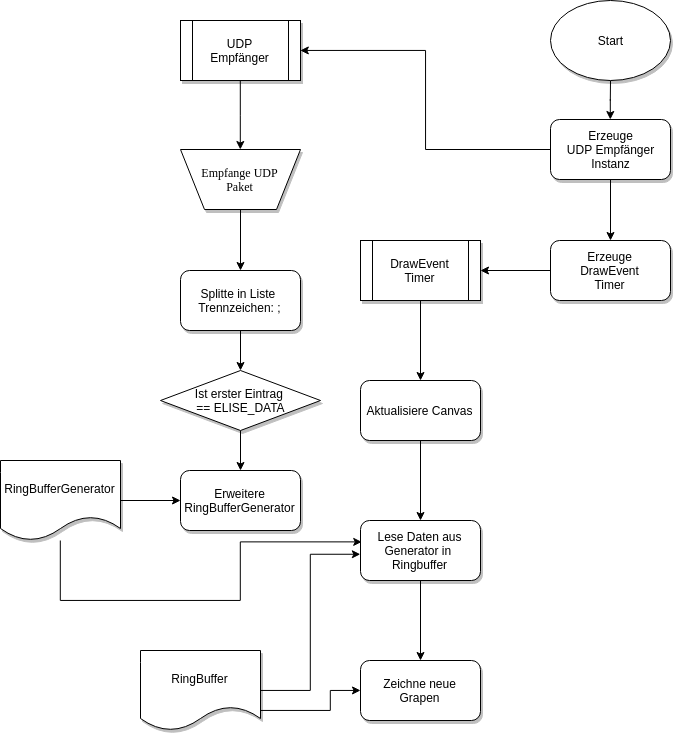
\includegraphics[width=\textwidth]{Images/ablauf_anzeige.png}
\end{minipage}
    \caption{Screenshot der Supervisor Ansicht}
    \label{fig:screen_soft1}
\end{figure}





% 3 Emotionsinduktion
\newpage
\section{Emotionsinduktion} \label{emotionsinduktion-sec}
\todo[inline]{Verantwortlich: Minas}


% Unterkapitel
\subsection{Ablauf} \label{ablauf-1}


\todo[inline]{Verantwortlich: Minas}


Der Ablauf der Emotionsinduktion lief wie folgt ab:

\begin{itemize}
\item[1.] Gl{\"u}ck (PowerPoint) $\rightarrow$ Kapitel 7.3.1
\item[2.] Langeweile (Video) $\rightarrow$ Kapitel 7.3.2
\item[3.] Frustration (Flashgame) $\rightarrow$ Kapitel 7.3.3
\item[4.] Langeweile (Spiel im Browser) $\rightarrow$ Kapitel 7.3.2
\end{itemize}

Nach jedem Szenario folgte ein sich automatisch {\"o}ffnender Fragebogen zum Szenario. 
Der Wechsel zwischen den Szenarien musste manuell statt finden.

% Unterkapitel 
\subsection{Fragebogen} \label{fragebogen-4}


\todo[inline]{Verantwortlich: Boris\\
- add picture of VR questionare (both dominat emotions and circumplex)}

F{\"u}r dieses Prototyp wurden zwei Arten von Frageb{\"o}gen benutzt. 
Der erste Typ ist sehr {\"a}hnlich mit dem von der zweite Prototyp. Es enth{\"a}lt in dem informativen Teil einen Text, wo es beschrieben wird, wie der Fragebogen ausgef{\"u}llt werden soll. Der andere Teil besteht aus vier Dropdown-Boxen von dreizehn Optionen, die zw{\"o}lf verschiedene Emotionen und einen als null oder neutral geltenden Zustand enthalten. Jede Dropdown-Box entspricht ein Viertelzeit der Szenario. Es soll zwischen die Optionen jeder Dropdown-Box gew{\"a}hlt werden, welche Emotion es am st{\"a}rksten empfindet wird, je nachdem, wann man es f{\"u}hlte, d.h. ob es das erste, zweite, dritte oder letzte Quartal der Zeit des Videos war, um die Emotion zu bew{\"a}ltigen. Unten gibt es ein Button wo man dr{\"u}cken kann, wenn man fertig ist. Allerdings hat man auch die M{\"o}glichkeit seine Wahl zu {\"a}ndern, auch wenn man sich schon im n{\"a}chsten Schritt befindet, indem man in diesem n{\"a}chsten Schritt auf den Zur{\"u}ck-Button dr{\"u}ckt und die gew{\"u}nschten {\"a}nderungen vornimmt. Hierf{\"u}r wird ein Widget Blueprint erstellt, die vier Dropdown-Boxen mit dem gew{\"u}nschten Anzahl an Optionen hinzugef{\"u}gt und die Labels von der unterschiedlichen Optionen der Dropdown-Boxen definiert. Ein Button ``next'' wird auch erstellt um zum n{\"a}chsten Fragebogen zu navigieren. Es wird auch eine zwischen Speicherungsfunktion in ein anderes Skript definiert, die hier aufgerufen wird, um die {\"a}nderung auch nach das dr{\"u}cken von dem ``next'' Button zu Speichern. Dabei wird vier Variablen definiert und die Werte von der gew{\"a}hlten Optionen werden ihnen zugewiesen. \\



\begin{figure}[H] \centering
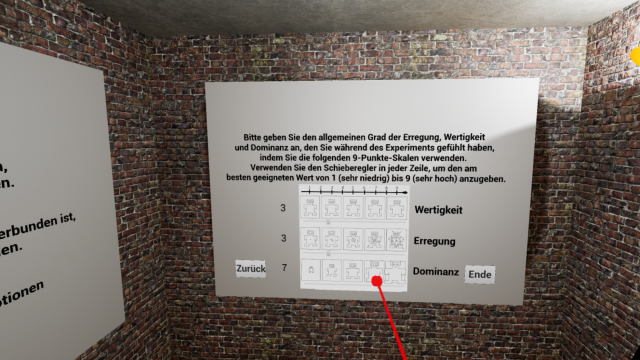
\includegraphics[width=\textwidth]{Images/Fragebogen_3.png} 
\caption{ Bild des Fragebogen-Teils, entsprechend dem circumplex-Modell. } 
\label{fig:fragenbogen4} \end{figure}



Der zweite Typ {\"a}hnelt dem ber{\"u}hmten Modell von James Russels ``circumplex'' \cite{russel_1980}. Es ist ein klassisches Modell mit einer kreisf{\"o}rmigen Struktur, die auf zwei senkrechten Diagonalen ruht. Die vertikale Achse, die die Erregung darstellt, und die horizontale Achse, die die Valenz darstellt. Das Zentrum des Kreises stellt eine neutrale Valenz und ein mittleres Erregungsniveau dar. Andere Emotionen werden auf jeder Ebene des Kreises dargestellt.  Hier wird ein weniger bekanntes Modell verwendet, das ``Self Assessment Manikin'' (SAM). Es besteht aus drei Reihen mit je f{\"u}nf Piktogrammen. Diese Piktogramme stellen den Zustand eines Gesichts nach verschiedenen Arten von Emotionen dar. So repr{\"a}sentiert der erste Bereich die Wertigkeit, der zweite die Erregung und der dritte die Dominanz. Eine Erkl{\"a}rung zu jedem dieser Begriffe ist ebenfalls neben dem Fragebogen enthalten, um die Testpersonen {\"u}ber diese W{\"o}rter aufzukl{\"a}ren.  Bei jeder Avatar und in der Mitte jeder der beiden Avatar befindet sich ein Checkbox.  So muss man f{\"u}r jede Zeile das Checkbox ausw{\"a}hlen, das ihrem emotionalen Zustand am besten entspricht. Man kann nur ein Checkbox pro Zeile markieren und man hat auch die M{\"o}glichkeit wie bei dem ersten Model seine Wahl zu {\"a}ndern. Es kann einfach mit Branch-Bedingungen realisieren werden.  Diese werden auch in eine Widget Blueprint wie f{\"u}r das erste Modell gemacht. Es gibt auch wieder die zwischen Speicherungsfunktion und das Button ``next''. Was neues hier kommt ist das Button ``back'' um wieder zum ersten Fragebogen zu navigieren. 



\begin{figure}[H] \centering
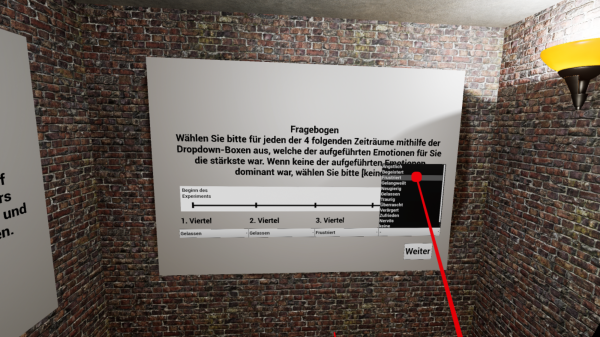
\includegraphics[width=\textwidth]{Images/Fragebogen_1.png} 
\caption{ Bild des Fragebogen-Teils, wo die dominierenden Emotionen abgefragt werden. } 
\label{fig:fragenbogen1} \end{figure}

% Unterkapitel 
\subsection{Szenarien} \label{szenarien-subsec}

\todo[inline]{Verantwortlich: Meryem}

% Unterkapitel 
\input{Part-1/3-Emotionsinduktion/3-Szenarien/1-glueck}

% Unterkapitel 
\input{Part-1/3-Emotionsinduktion/3-Szenarien/2-langeweile}

% Unterkapitel 
\input{Part-1/3-Emotionsinduktion/3-Szenarien/3-frust}


% 4 Messreihe
\newpage
\section{Messreihe} \label{messreihe-sec}
\todo[inline]{Kevin, Artur}




% 5 Mustererkennung
\newpage
\section{Mustererkennung} \label{mustererkennung-sec}

\todo[inline,color=green!40]{Verantwortlich: Artur\\
- RfP}

In diesem Kapitel werden alle Schritte entlang der ERC (vgl. Kapitel \ref{emotion-recogniton-chain}) konkretisiert und es wird detailreich beschrieben, wie wir vorgegangen sind. \\


% 1 Datenerfassung
\subsection{Datenerfassung} \label{datenerfassung-1}


In Kapitel \ref{messreihe-1-sec} wurde das verwendete Datenset bereits detailiert beschrieben, sodass hier darauf verzichtet wird. \\

% 2 Vorverarbeitung
\subsection{Vorverarbeitung} \label{vorverarbeitung-1}

Wie bereits in Kapitel \ref{vorverarbeitung-0} beschrieben, ist das Ziel der Vorverarbeitung die ”Verbesserung” der Daten f{\"u}r die nachfolgenden Schritte der ERC.
Im Rahmen des ELISE Projektes wurden Normalisierungstechniken auf dem gesamten Datensatz angewendet. 
Wir haben insbesondere die Standardnormalisierung verwendet, welche den Mittelwert der Daten auf Null setzt und die Einheitsvarianz ergibt \cite{grus15}. 
Die Formel f{\"u}r die Standardnormierung lautet:
\begin{equation} 
\Large{ {x'={\frac {x-{\overline {x}}}{\sigma }}} } 
\label{equ:norm} \end{equation} %\vspace{0.5cm}

wobei $ x $ ein Datenpunkt eines Sensorkanales, $ \overline{x} $ ist der Durchschnitt der Gesamtheit f{\"u}r diesen Sensorkanal und $ \sigma $ ist die entsprechende Standardabweichung. \\

% 3 Segmentation
\subsubsection{Segmentation} \label{segmentation-0}

Ziel dieses Schrittes ist es, Teile von Daten zu identifizieren, welche wichtige Informationen über die zu erkennenden Emotionen enthalten. 
Dies geschieht durch Filtern der Daten und Ausschließen von Segmenten, die für das Klassifizierungsproblem nicht relevant sind.
Zusätzlich wird die zu verarbeitende Datenmenge reduziert, indem Segmente eines Zeitfensters fester Größe aus den Daten extrahiert werden.
Diese Vorgeheisweise ist heute in der Praxis besonders wichtig, da sonst hardwarebedingte Einschränkungen die zu verarbeitende Datenmenge begrenzen könnten. \\

% 4 Merkmalsextraktion
\subsection{Merkmalsextraktion} \label{merkmalsextraftion-1}

Wie bereits in Kapitel \ref{merkmalsextraktion-subsubsec} beschrieben, ist das Ziel der Merkmalsextraktion Charakteristiken und Merkmale in den Daten zu finden, die für das
Klassifizierungsproblem von möglichst hoher Relevanz sind. Im Rahmen des ELISE Projektes haben wir verschiedene Vorgehensweisen angewendet. Im den folgenden Unterkapiteln werden diese vorgestellt. \\



% Unterkapitel 
\subsubsection{Handgefertigte Merkmale} \label{hc-features-1}
Der handgefertigten Merkmal Ansatz (enlg. "hand-crafted features approach") besteht in der Berechnung relativ einfacher Merkmale von denen vermudetet wird, dass sie für das Klassifizierungsproblem der Eingangssignale relevant sein können. Diese Vorgehensweise hat den Vorteil des einfachen Aufbaus als auch der relativ geringen benötigten Rechenleistung, wobei potentiell gute Klassifizierungsergebnisse erwarten werden. \\


Obwohl frühere Forschungsarbeiten schon handgefertigte Merkmale zur Emotionserkennung unter mithilfe physiologischer Signale getestet haben (vgl. \cite{martinez_ieee_2013}), wurde dieser Ansatz noch nie für die Erkennung dieser spezifischen Emotionen unter Verwendung dieser Kombination von Sensoren getestet.
Zusätzlich haben wir zuerst handgefertigte Merkmale getestet, um ein Basisergebnis zu liefern, mit der die Ergebnissen der anderen Ansätze vergleichen werden können.
Handgefertigte Merkmale sind in der Regel entweder einfache statistische Werte, Fourier-basierte oder selbstentwickelte Merkmale sein, die aufgrund von Vorkenntnissen der Daten verwendet werden. 
Diese Arbeit wurden statistische, Fourier-basierte und selbstentwickelte Merkmale getestet. \\

\textbf{Statistische Merkmale \\}
Die Tabelle \ref{tab:statistische} fasst die elf verschiedenen und in der Studie verwendeten statistischen Merkmale zusammen. Wir bezeichnen $\mathbf{x} = (x_1, x_2, ...., x_T) $ als Vektor, der die in einem Datenzeitfenster der Länge $T$ enthaltenen Sensorwerte für einen Sensorkanal darstellt. 


\begin{table}[h]
\begin{tabular}{| l | p{12.5cm} |}
\hline
    \textbf{Merkmalname}     &  \textbf{Definition}  \\ \hline
    
    Durchschnitt         & \vspace{0.01cm}
    $ mean(\mathbf{x}) =$ \Large{$\frac{1}{T} \sum_{k=1}^T (x_k) $} \\[0.5cm] \hline 
    
    Standard-Abweichung        & \vspace{0.01cm}
    $ \sigma(\mathbf{x}) =$ \Large{$ \sqrt{ \frac{1}{T} \sum_{k=1}^{T}{(x_k - \mu)^{2}} } $ } \\[0.5cm] \hline
    
    Maximum                   & \vspace{0.01cm}
    $ max(\mathbf{x}) = \max(x_{1},x_{2},\dots ,x_{T}) $
    \\[0.5cm] \hline
    
    Minimum                   & \vspace{0.01cm}
    $ min(\mathbf{x}) = \min(x_{1},x_{2},\dots ,x_{T}) $
    \\[0.5cm] \hline
    
    Amplitude                 & \vspace{0.01cm}
    $ A(\mathbf{x}) = max(\mathbf{x}) - min(\mathbf{x}) $ 
    \\[0.5cm] \hline
    
    25/50/75\% Perzentil      & Wert einer Menge, unter dem 25/50/75\% der Werte aus der Menge fallen. \\ \hline
    
    Interquartiler Bereich    & Differenz zwischen dem 75. und 25. Perzentil.
    \\ \hline
     
    Schräge                   & \vspace{0.01cm}
    $ \gamma _{1}(\mathbf{x}) = \operatorname{E}$ \Large{$\left[\left({\frac {X-\mu }{\sigma }}\right)^{3}\right]$ \normalsize{$=$} ${\frac {\mu _{3}}{\sigma ^{3}}}$ \normalsize{$=$} ${\frac {\operatorname {E} \left[(X-\mu )^{3}\right]}{ (\operatorname {E} \left[(X-\mu )^{2}\right])^{3/2}}}$ \normalsize{$=$} ${\frac {\kappa _{3}}{\kappa _{2}^{3/2}}} $} \vspace{0.2cm}
    \\[0.3cm] \hline
     
    Kurtosis                  & \vspace{0.01cm}
    $ \operatorname {Kurt}[\mathbf{x}] = \operatorname{E} $ \Large{$\left[\left({\frac {X-\mu }{\sigma }}\right)^{4}\right]$ \normalsize{$=$} ${\frac {\mu _{4}}{\sigma ^{4}}}$ \normalsize{$=$} ${\frac {\operatorname {E} [(X-\mu )^{4}]}{(\operatorname {E} [(X-\mu )^{2}])^{2}}} $} \vspace{0.2cm}
    \\[0.3cm] \hline
\end{tabular} 
\caption{Statistische Merkmale, die im Rahmen des ELISE-Projektes verwendet wurden. } \label{tab:statistische}
\end{table} 


\textbf{Fourier-basierte Merkmale \\}
\todo[inline]{Artur: \\
- Muss ich noch schreiben $\rightarrow$ Warten auf Julian's Antwort. \\}


\textbf{Selbstentwickelte Merkmale \\}
Es wurden zwei eigene Merkmale definiert: Nulldurchgang (engl. "zero crossing") und Anzahl der Spitzen (engl. "number of peaks"). Im Folgendem werden diese beiden Merkmale detailiert beschrieben. \\

Das Nulldurchgang-Merkmal zählt die Häufigkeit, mit der das Signal eines Sensorkanals in einem Zeitfenster die Nulllinie überschreitet.
Alle Sensorsignale wurden durch Normierung verarbeitet (vgl. Kapitel xxx) und damit wurden alle Mittelwerte auf Null zentriert.
Um zu vermeiden, dass Rauschen entlang der Nulllinie in dem Merkmal gezählt wird, wird nur ein Nulldurchgang in einer bestimmten Zeitspanne gezählt. \\


Das Spitzenzähler-Merkmal bestimmt die Anzahl von loklanen Hochpunkten im Zeitsignal.
Alle lokalen Maximen sind durch einen Onset (Startpunkt), eine Spitze und einen Offset (Endpunkt) gekennzeichnet (vgl. Abbildung \ref{fig:peaks}). 
Jedes Vorkommen einer Onset/Offset-Paarung wird hierbei als Spitze gezählt.
Onsets, Spitzen und Offsets werden durch die folgenden Operationen identifiziert \cite{BSc_Gouverneu}:

\begin{itemize} %[noitemsep]
  \item Ein Onset wird bestimmt, wenn der Wert des Signals an diesem Punkt nicht negativ ist und die Differenz zwischen ihm und dem nächsten größer als ein vordefinierter Schwellenwert (engl. "threshold") ist.

  \item Ein Offset wird bestimmt, wenn der Wert des Signals kleiner als der Wert des zuletzt gesetzten Onsets ist.

  \item Das lokale Maximum zwischen einem Onset und Offset wird als Spitze bezeichnet.
\end{itemize} \vspace{0.2cm}


\begin{figure}[h] \centering{
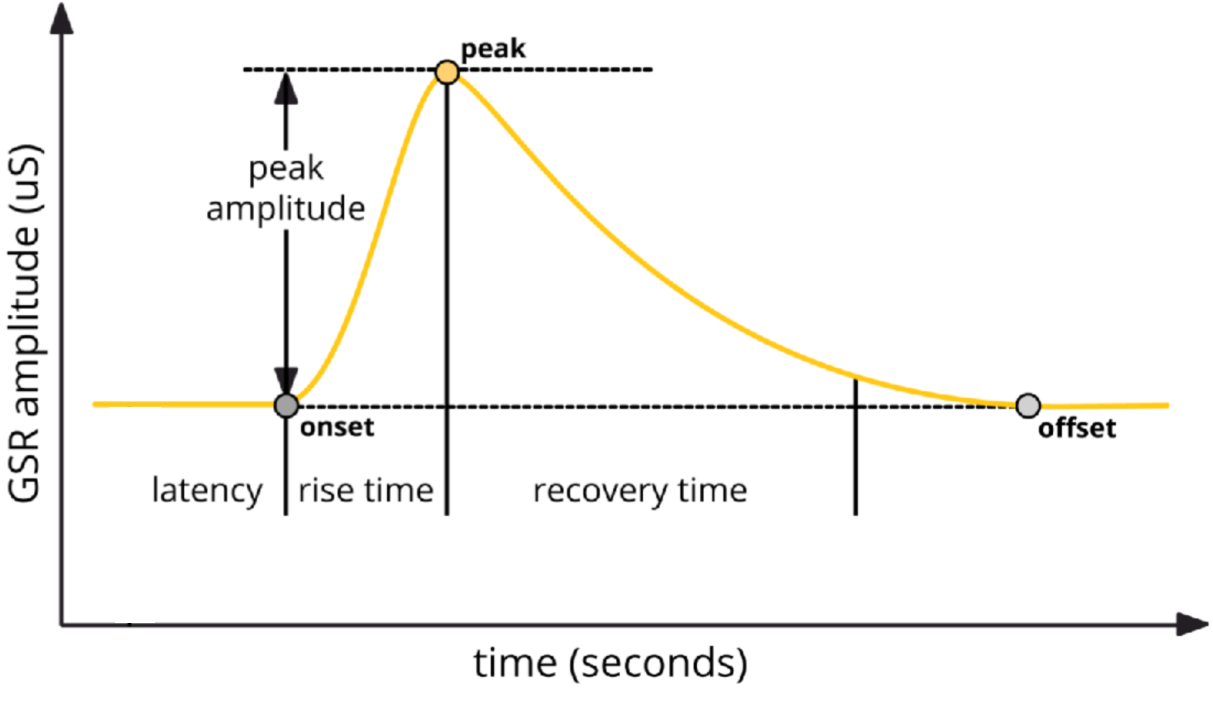
\includegraphics[width=11cm]{Images/peaks.png}}
\caption{ Spitzenzähler: Onset (Startpunkt), Spitze und Offset (Endpunkt). Jedes Paar von Onset/Offset erhöht die Anzahl der Spitzen um eins.} 
\label{fig:peaks} \end{figure} \vspace{0.5cm}


Jedes handgefertigte Merkmal wird auf einem Zeitfenster von Daten für jeden Sensorkanal unabhängig voneinander angewendet. 
Jedes Zeitfenster ist daher 117 Merkmalen zugeordnet (9 Sensorkanäle multipliziert mit 13 Merkmalen). \\





% Unterkapitel 
\subsubsection{Codebook Approach} \label{ca-1}


Die bisherige Methodik mit handgefertigten Merkmalen ist klassisch für den überwachten Lernansatz. 
Es existieren aber auch einige Nachteile. 
Das Hauptproblem besteht darin, dass nicht sichergestellt werden kann, dass die gewählten Merkmale die besten Klassifizierungsergebnisse erzielen. Damit besteht immer die Gefahr, dass möglicherweise andere Merkmalen bessere Ergebnisse liefern würden, diese handgefertigten Merkmale aber die  nicht gefunden wurden. Dieses Risiko besteht insbesondere bei der physiologischen Signalverarbeitung zur Emotionserkennung, wo die Struktur der Daten noch recht unbekannt und allgemein komplex ist. 
Eine weitere Schwierigkeit besteht darin, relevante selbstentwickelte Features ohne Expertenwissen über die Daten zu finden.
Darüber hinaus wurden noch keine gut funktionierenden State-of-the-Art handgefertigten Merkmale identifiziert.
Aus diesen Gründen ist es interessant halbautomatische und unüberwachter Ansätze der Merkmalsextraktion zu verwenden und zu testen. \\


K. Shirahama et al. \cite{kimiaki_codebook_approach_2016} schlugen eine unüberwachte Merkmalsextraktionsmethode namens Codebook Approach (CA) vor, um Merkmale aus 1D-Zeitreihensignalen zu erzeugen.
Der CA hat den Vorteil, dass formbasierte Merkmale gefunden werden können, die für das Problem der Emotionserkennung relevant sind, aber weder offensichtlich noch leicht als Mensch zu interpretieren sind. 
Der CA besteht aus drei Schritten, die in den folgenden Abschnitten erläutert werden: Codebuchkonstruktion (engl. "codebook construction"), Codewortzuordnung (engl. "codeword assignment") und der anschließenden Klassifizierung. \\


\textbf{Codebuchkonstruktion \\}
Ziel dieses Schrittes ist es, Teilsequenzen (sogenannte "Codewörter") zu bestimmen, die für die 1D-Eingangssensorik charakteristisch sind. 
Dies wird erreicht, indem Zeitfenster aus dem ursprünglichen Datensatz für jeden Sensorkanal unabhängig voneinander nach dem im Kapitel \ref{segmenation-1} definierten Segmentierungsansatz extrahiert werden.
Aus jedem so erhaltenen Zeitfenster der Größe $T$ werden kleinere Segmente der Größe $\alpha$ unterteilt.
Ein Clustering-Algorithmus wird dann auf die Menge der Segmente $\alpha$ angewendet, um Clusterzentren zu finden.
Nach der Konvergenz werden die Clusterzentren als Codewörter betrachtet und zum Aufbau einer Sammlung von Codewörtern mit dem Namen ``Codebuch'' verwendet, wie in Abbildung \ref{fig:ca_construction} aus \cite{kimiaki_codebook_approach_2016} dargestellt. 
Die Anzahl der Codewörter (d.h. die Größe des Codebuchs oder die Anzahl der Cluster) ist ein Hyperparameter des Verfahrens. Im Rahmen dieser Arbeit wurde ein k-means Clustering-Algorithmus verwendet, um die Codewörter auf den ELISE-Daten zu erhalten. \\



% 5 Klassifikation
\subsection{Klassifikation} \label{klassifikation-1}

Wie bereits in Kapitel \ref{grundlagen-klassifikation-0} beschrieben ist das Ziel der Klassifizierung ein Klassifizierungsmodell zu trainieren, das in der Lage ist, Objekte in den Daten in die entsprechende Klasse zuzuordnen. Die Klassen entsprechen hierbei den Emotionen, die erkannt werden sollen: Glück, Langeweile, Frustation und andere (d.h. alle Emotionen, die nicht Glück, Langeweile oder Furstation entsprechen). \\

Als erstes wird der Datensatz in ein Trainigs- und Testset  aufgeteilt. 
Es gibt keine festgelegten Regeln über die Proportionen der Sets. 
Im Allgemeinen wird das Trainingsset aber größer als das Testset gewählt.
Da die Leistungen des Klassifikators jedoch stark von der gewählten Aufteilung abhängen, ist es wichtig, sicherzustellen, dass dieser Schritt richtig durchgeführt wird.
Bei einem Datensatz mit mehreren Probanden empfiehlt sich für die Aufteilung zwischen Trainings- und Testsets die Durchführung einer Leave-One-Subjekt-Out-Cross-Validierung (LOSOCV).
Die Idee besteht darin, $N$ verschiedene Aufteilungen des Datensatzes vorzunehmen, wobei $N$ die Anzahl der Personen ist, die Daten für den Datensatz bereitgestellt haben. 
Für jeden dieser Splits wird der Testset aus den Daten eines Probanden aufgebaut, während die Daten der anderen Probanden das Trainingsset bilden. 
Anschließend wird ein Klassifizierer erstellt und ausgewertet. Dies wird für alle Probanden wiederholt, d.h. $N$ mal.
Die so erhaltenen $N$-Bewertungskennzahlen (eine pro Proband) können dann gemittelt werden, um eine Gesamtbewertung des Modells zu erhalten.
Es ist wichtig zu beachten, dass der LOSOCV-Ansatz bei einer hohen Anzahl von Probanden sehr rechenintensiv sein kann. \\

\begin{figure}[h] \centering{
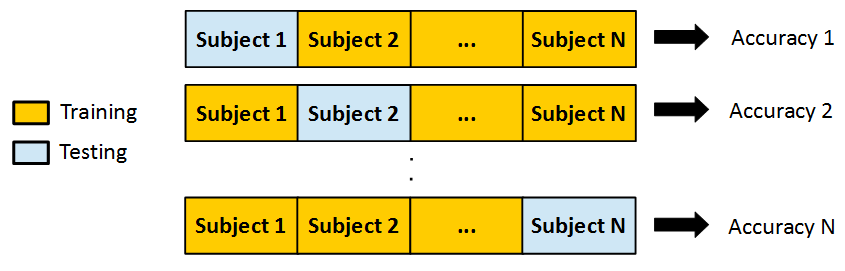
\includegraphics[width=15cm]{Images/LOSOCV.png} 
\caption{ Leave-One-Subjekt-Out-Cross-Validation (LOSOCV): $N$ entspricht der Anzahl der Probanden. Für jeden Split wird ein Testset aus den Daten eines Probanden aufgebaut, während die Daten der anderen Probanden einen Trainingsset bilden. Dieser Vorgang wird für die Daten jedes Probanden durchgeführt. }}
\label{fig:losocv} \end{figure} \vspace{0.5cm}

% 6 Ergebnisse
\newpage
\section{Ergebnisse} \label{ergenisse-sec}
\todo[inline]{Artur}



% Unterkapitel 
\subsubsection{Hand-gefertigte Merkmale} \label{hc-features-subsubsec}







% Unterkapitel 
\subsection{Ergebnisse des Codebook Approach} \label{ergebnisse-codebook-approach-subsec}


{\"A}hnlich wie bei den handgefertigten Merkmalen haben wir die Daten mit einer Normalisierungstechnik vorverarbeitet und dann die Segmentierung verwendet. Die Zeitfensterparameter sind identlisch wie bei der Studie mit den handgefertigten Merkmalen.
F{\"u}r die Klassifizierung haben wir SVM mit Soft-Margins und dem RBF-Kernel benutzt. 
Um die optimalen Parameter des SVM-Klassifikators zu bestimmen (z.B. Soft-Margin $C$ und Kernelparameter $\gamma$), wurde hier wieder die Gitter-Suche angewendet. \\


Die Ergebnisse, die wir mit dem CA mit fester Zuordnung (hard assignment) und $C = 8$, $\gamma = 0,002$ f{\"u}r jeden Probanden erhielten, waren 52\%, 38\% und 38\%, was einem Durchschnitt von 42,67\% entspricht. CA mit Soft-Assignment wurden ebenfalls getestet, lieferte aber schlechtere Ergebnisse als CA mit Hard-Assignment. In diesem speziellen Datensatz schneidet der CA also schlechter ab als die handgefertigten Merkmale.








\subsection{Ergebnisse der Deep Neutral Networks} \label{ergebnisse-dnn}

Die Verwendung von DNNs zur Extraktion von Merkmalen (z.B. Multi-Layer-Perceptron, Convolutional Neural oder Long-Short-Term-Memory Networks) wurden zwar intensiv getestet (siehe \cite{bscschnieber18}), diese Ansätze erreichten aber leider nicht so gute Ergebnisse, wie z.B. die oben vorgestellten Ergebisse der handgefertigten Merkmale. Die beste Performance erreichten LSTM mit einem F1-Score von 47,99\%. \\



% Unterkapitel
\subsection{Analyse der Ergebnisse} \label{analyse-subsec}











% Part 4
\newpage
\fancyhf{} \cfoot{\thepage} \rhead{\leftmark \hspace{0.2cm} PART III} % Header Part 4
\part{Dritter Prototype}
\addtocontents{toc}{\protect\mbox{}\protect\hrulefill\par}


% 1 Systementwurf
\section{Systementwurf und Konzept} \label{systementwurf-4}
\todo[inline]{Verantwortlich: Kevin, Jonas}



% Unterkapitel 
\subsection{Anforderungen} \label{anfoderungen-1}

Auf Grundlage der Ziele des Forschungsprojektes ELISE und dem Sichten und Vergleichen von mehr als 30 wissenschaftlichen Veröffentlichungen der letzten 15 Jahre, ergeben sich bestimmte
Anforderungen für den Entwurf eines eigenen Emotionserkennungssystems. Einige wissenschaftliche Veröffentlichungen sind dabei nicht außer Acht zu lassen. Die Foscher von T.
Sharma, S. Bhardwaj und H. B. Maringanti haben in ihrer Veröffentlichung Emotion Estimation
using Physiological Signals versucht, mit Hilfe von GSR, Herzschlagrate,
BVP und der Temperatur Aufschluss über die Emotionen Zorn, Angst, Freude und Traurigkeit
durch Stimulation verschiedener Songs und Videos zu erhalten. Sie erforschten, in
welchen Fällen sich die Körperleitfähigkeit je nach emotionalem Ausdruck unterschiedlich
verhält. H. F. Garcia, A. A. Orozco und M. A. Alvarez versuchten in ihrer Arbeit Dynamic
physiological signal analysis based on Fisher kernels for emotion recognition durch unterschiedliche Klassifizierungsmodelle, die Signale von EEG, EOG, EMG (Elektromyografie),
GSR, Atmung und Temperatur zu analysieren. Dafür wurden 32 Probanden,
die ein 40-minütiges Video mit Musikausschnitten ansahen, aufgezeichnet und ausgewertet.
Durch ein automatisches Regressionsprozess-Modell verbesserten sie dynamische Merkmale
und weitere aufgezeichnete Signale für eine weiterführende Auswertung.
Die Emotionserkennung erfolgte bis vor einigen Jahren in Verbindung mit zusätzlichen Kameras
und Software zur Gesichtsmimik-Erkennung oder Stimmerkennung, nicht jedoch mit
einer reinen Aufnahme von Körpermesswerten. In ELISE sollen insbesondere die lernrelevanten Emotionen Langweile, Frustration, Verwirrung sowie Engagement und Freude erkannt
werden. Die Hardware-Architektur muss auch in diesem Fall wieder das Ziel erfüllen, dass
das Gefühl der Immersion nicht gestört wird. Das heißt, dass das System zur Erkennung von
lernrelevanten Emotionen an möglichst wenigen Stellen am Körper mit zusätzlicher Sensorik
angebracht wird.
Auf Basis der Literaturrecherche, wie in der Bibliographie ausgewiesen, sind folgende Sensoren
zur Aufnahme der lernrelevanten Emotionen ausgewählt worden:

• Gehirnaktivität (EEG)
• Augenbewegung (EOG)
• Blutvolumenpuls (BVP)
• Sauerstoffsättigung im Blut (PPG)
• Hautleitfähigkeit (GSR)
• Körpertemperatur

Da die Sensorwerte zum Mikrocontroller aufgrund ihres räumlichen Abstandes über den
Bus übertragen werden, unterliegen diese Werte den Zeitanforderungen des Datenbusses.
Hier ist zu überprüfen, welches Buskonzept den Zeitanforderungen gewachsen ist.
Um den Aufwand für den Benutzer gering zu halten und die Immersion nicht zu stören,
wird versucht, die Sensorik direkt an der VR-Brille anzubringen. Für die EEG- und
EOG-Sensoren ist dies sowieso notwendig, da diese Messungen lediglich am Kopf stattfinden
können. Zudem soll das Endsystem echtzeitfähig sein, um in der späteren Anwendung
Änderungen und Fluktuationen der Emotionen erkennen zu können und die Schulungen auf
den Lernenden anzupassen. Das Emotionserkennungssystem soll mobil anwendbar sein, da
neuere Versionen der HTC Vive VR-Brille in Zukunft den kabellosen Betrieb unterstützen.
Auch aus diesem Grund ist die Kompaktheit, Energieeffizienz und die Datenübertragung der
einzelnen Sensoren und die Datenübertragung des späteren Gesamtsystems, die ebenfalls
kabellos stattfinden soll, von großem Interesse. Eine mögliche Stelle zur Unterbringung des
Gesamtsystems wäre am Hinterkopf des Probanden, da dort der nötige Platz vorhanden ist
und erforderliche Befestigungsstellen am Kopfband der HTC Vive von Vorteil sind.



% Unterkapitel 
\subsection{Konzept} \label{konzept-1}

Auf Abbildung 1 kann man das Konzept der Architektur erkennen, Dies ist zur besseren Anschauung stark vereinfacht. Hierbei bildet der Mikrocontroller das zentrale Element, welches die einzelnen Sensoren anbindet, steuert und die Messsignale grob zur besseren Auswertung verarbeitet. Zur besseren und möglichst in Echtzeit stattfindeten Verarbeitung werden die Daten an einen externen Rechner weitergeleitet. In der Abbildung findet diese Weiterleitung Drahtlos mittels Bluetooth statt. Es wurden in den verschiedenen Prototypen für diese Zwecke sowohl Bluetooth als auch WLAN verwendet. Für die Teilsysteme EEG und EOG wurden schon einfache Physische Filter auf den Leiterplatten vorgesehen, welche die analogen Signale vorberarbeiten, bevor dies von einem AD-Wandler digitalisiert werden. Da die Elektroden für die EEG und EOG Messung nur am Kopf angebracht werden können, empfiehlt es sich die übrigen festgelegten Werte ebenfalls am Kopf zu messen. Um die Messung für möglichst viele Personen mit unterschiedlichen Kopfformen zu ermöglichen wurde zuerst ein elastisches Kopfband und später eine flexible Maske verwendet. All dies wurde für eine spätere Verwendung mit (unter) einer VR-Brille designet. 





% Unterkapitel
\subsection{Hardwareauswahl} \label{hardwareauswahl-1}

Bei der Wahl der richtigen Hardware zur Aufnahme, Verarbeitung und Weiterleitung von
biomedizinischen Signalen, sind die reinen Hardwarekosten von untergeordneter Bedeutung.
Jedoch sollte das Budget für das spätere Gesamtsystem einen gewissen Rahmen nicht überschreiten,
um auch die aufkommenden Endkosten in Verbindung mit einer VR-Brille und der
benötigten Hardware zur Darstellung der Lerninhalte in einem gewissen Rahmen zu halten.
Die Bandbreite der angebotenen Systeme von unterschiedlichen Mikrocontrollern ist dabei
sehr groß. Zu Beginn einer geeigneten Neubeschaffung sollten, wie bei jedem IT-Projekt, die
zuvor genannten Anforderungen an das System betrachtet werden und daraus Auswahlkriterien
für die geeignete Hardware gewählt werden.

% Unterkapitel 
\input{Part-1/1-Systementwurf/3-Hardwareauswahl/1-auswahlkriterien}

% Unterkapitel 
\input{Part-1/1-Systementwurf/3-Hardwareauswahl/2-festlegung-hardware}



% Unterkapitel
\subsection{Hardwarearchitektur} \label{hardwarearchitektur-subsec}



% Unterkapitel
\input{Part-4/1-Systementwurf/4-Hardwarearchitektur/1-gsr}

% Unterkapitel
\input{Part-4/1-Systementwurf/4-Hardwarearchitektur/2-temperatur}

% Unterkapitel 
\input{Part-4/1-Systementwurf/4-Hardwarearchitektur/3-pulsoximeter}

% Unterkapitel 
\input{Part-4/1-Systementwurf/4-Hardwarearchitektur/4-eeg}

% Unterkapitel 
\input{Part-4/1-Systementwurf/4-Hardwarearchitektur/5-eog}

% Unterkapitel
\input{Part-4/1-Systementwurf/4-Hardwarearchitektur/6-datenuebertragung}



% Unterkapitel 
\subsection{Programmierung} \label{programmierung-subsec}

Die Programmierung des dritten Prototypen basiert im wesentlichen auf der des zweiten Protoypen, da sich in Bezug auf die Hardware nur die GSR-Schaltung geändert hat. Wie auch bei vorherigen Prototypen erfolgte die Programmierung mit Hilfe der Arduino Plattform und der durch die Hersteller schon zur Verfügung gestellten Bibliotheken.





% Unterkapitel 
\subsection{Aufnahme der {\"u}bertragenen Daten} \label{aufnahme-daten-subsec}

Beim dritten Prototypen wurden die Daten wieder drahtlos übertragen. Im Gegensatz zum ersten Prototypen kam hier aber nicht mehr ein Bluetooth-Modul zum Einsatz, sondern das im ESP32 integrierte WLAN-Modul. In den mit diesem Prototypen durchgeführten Messungen wurden die Daten mittels WireShark aufgenommen und abgespeichert. Diese Daten wurden später zur Datenanalyse in eine CSV-Datei umgewandelt. Zur Übertragung wurde das zuvor schon beschriebene UDP-Protokoll  verwendet. An dieser Stelle sei noch einmal Erwähnt, das alle Daten mit einer Abtastrate von 250 Samples pro Sekunde gemessen wurden. Die einzige Ausnahme hier ist die Temperatur, die lediglich mit einer Rate von 3,3 Samples pro Sekunde gemessen wurde. 




% 2 Realisierung
\newpage
\section{Realisierung} \label{realisierung-4}


Für den ersten Versuch mit Testpersonen wurden die Experimente zur Emotionsinduktion zu einem Gesamtexperiment verbunden. Dabei wurde darauf geachtet einen möglichst automatisierten Testablauf zu erreichen, so dass die Testperson möglichst unbeeinflusst von äußeren Reizen oder den Aktionen des Testleiters bleibt. Dazu wurde eine automatisierte Webanwendung programmiert, die der Versuchsperson alle Anweisungen und Experimente präsentiert (siehe Abbildung \ref{fig:screen_soft1}). Der Versuchsleiter wiederum kann durch eine, ebenfalls webbasierte, Kontrollkonsole Einfluss auf das Experiment nehmen, in dem er zum Beispiel den Ablauf stoppen oder Schritte überspringen kann (siehe Abbildung \ref{fig:screen_soft1}).\\

Die Ablaufkontrolle erfolgt über den Flask Webserver, der die Website darstellt. Zur Steurung können einfach URLs auf dem Server mittels einer GET bzw. POST Anfrage aufgerufen werden und so Steuerbefehle übermittelt werden. \\

Die Bilder, die dem Probanden angezeigt werden, wie auch die Spiele, die er spielen soll, sind nahtlos in die Website eingebettet. Dies ist möglich, dadurch, dass es sich zum einen um eine Javascript Anwendung und zum anderen um eine Flash Anwendung handelt. Die Flash Anwendung wurde zur einfacheren Handhabung so präpariert, dass das Menü entfernt wurde und das Spiel direkt mit dem ersten Level beim Laden startet. \\

\begin{figure}[h]
    \centering
\begin{minipage}[t]{0.9\textwidth}
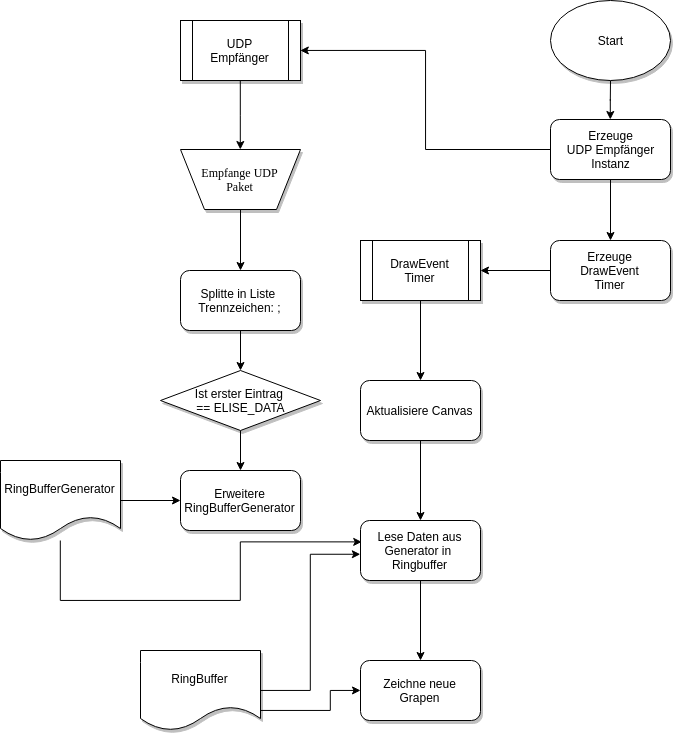
\includegraphics[width=\textwidth]{Images/ablauf_anzeige.png}
\end{minipage}
    \caption{Screenshot der Supervisor Ansicht}
    \label{fig:screen_soft1}
\end{figure}





% 3 Emotionsinduktion
\newpage
\section{Emotionsinduktion} \label{emotionsinduktion-4}
\todo[inline]{Verantwortlich: Minas}


% Unterkapitel
\subsection{Ablauf} \label{ablauf-1}


\todo[inline]{Verantwortlich: Minas}


Der Ablauf der Emotionsinduktion lief wie folgt ab:

\begin{itemize}
\item[1.] Gl{\"u}ck (PowerPoint) $\rightarrow$ Kapitel 7.3.1
\item[2.] Langeweile (Video) $\rightarrow$ Kapitel 7.3.2
\item[3.] Frustration (Flashgame) $\rightarrow$ Kapitel 7.3.3
\item[4.] Langeweile (Spiel im Browser) $\rightarrow$ Kapitel 7.3.2
\end{itemize}

Nach jedem Szenario folgte ein sich automatisch {\"o}ffnender Fragebogen zum Szenario. 
Der Wechsel zwischen den Szenarien musste manuell statt finden.

% Unterkapitel 
\subsection{Fragebogen} \label{fragebogen-4}


\todo[inline]{Verantwortlich: Boris\\
- add picture of VR questionare (both dominat emotions and circumplex)}

F{\"u}r dieses Prototyp wurden zwei Arten von Frageb{\"o}gen benutzt. 
Der erste Typ ist sehr {\"a}hnlich mit dem von der zweite Prototyp. Es enth{\"a}lt in dem informativen Teil einen Text, wo es beschrieben wird, wie der Fragebogen ausgef{\"u}llt werden soll. Der andere Teil besteht aus vier Dropdown-Boxen von dreizehn Optionen, die zw{\"o}lf verschiedene Emotionen und einen als null oder neutral geltenden Zustand enthalten. Jede Dropdown-Box entspricht ein Viertelzeit der Szenario. Es soll zwischen die Optionen jeder Dropdown-Box gew{\"a}hlt werden, welche Emotion es am st{\"a}rksten empfindet wird, je nachdem, wann man es f{\"u}hlte, d.h. ob es das erste, zweite, dritte oder letzte Quartal der Zeit des Videos war, um die Emotion zu bew{\"a}ltigen. Unten gibt es ein Button wo man dr{\"u}cken kann, wenn man fertig ist. Allerdings hat man auch die M{\"o}glichkeit seine Wahl zu {\"a}ndern, auch wenn man sich schon im n{\"a}chsten Schritt befindet, indem man in diesem n{\"a}chsten Schritt auf den Zur{\"u}ck-Button dr{\"u}ckt und die gew{\"u}nschten {\"a}nderungen vornimmt. Hierf{\"u}r wird ein Widget Blueprint erstellt, die vier Dropdown-Boxen mit dem gew{\"u}nschten Anzahl an Optionen hinzugef{\"u}gt und die Labels von der unterschiedlichen Optionen der Dropdown-Boxen definiert. Ein Button ``next'' wird auch erstellt um zum n{\"a}chsten Fragebogen zu navigieren. Es wird auch eine zwischen Speicherungsfunktion in ein anderes Skript definiert, die hier aufgerufen wird, um die {\"a}nderung auch nach das dr{\"u}cken von dem ``next'' Button zu Speichern. Dabei wird vier Variablen definiert und die Werte von der gew{\"a}hlten Optionen werden ihnen zugewiesen. \\



\begin{figure}[H] \centering
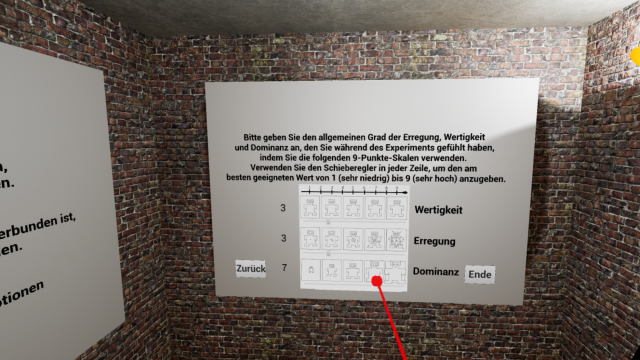
\includegraphics[width=\textwidth]{Images/Fragebogen_3.png} 
\caption{ Bild des Fragebogen-Teils, entsprechend dem circumplex-Modell. } 
\label{fig:fragenbogen4} \end{figure}



Der zweite Typ {\"a}hnelt dem ber{\"u}hmten Modell von James Russels ``circumplex'' \cite{russel_1980}. Es ist ein klassisches Modell mit einer kreisf{\"o}rmigen Struktur, die auf zwei senkrechten Diagonalen ruht. Die vertikale Achse, die die Erregung darstellt, und die horizontale Achse, die die Valenz darstellt. Das Zentrum des Kreises stellt eine neutrale Valenz und ein mittleres Erregungsniveau dar. Andere Emotionen werden auf jeder Ebene des Kreises dargestellt.  Hier wird ein weniger bekanntes Modell verwendet, das ``Self Assessment Manikin'' (SAM). Es besteht aus drei Reihen mit je f{\"u}nf Piktogrammen. Diese Piktogramme stellen den Zustand eines Gesichts nach verschiedenen Arten von Emotionen dar. So repr{\"a}sentiert der erste Bereich die Wertigkeit, der zweite die Erregung und der dritte die Dominanz. Eine Erkl{\"a}rung zu jedem dieser Begriffe ist ebenfalls neben dem Fragebogen enthalten, um die Testpersonen {\"u}ber diese W{\"o}rter aufzukl{\"a}ren.  Bei jeder Avatar und in der Mitte jeder der beiden Avatar befindet sich ein Checkbox.  So muss man f{\"u}r jede Zeile das Checkbox ausw{\"a}hlen, das ihrem emotionalen Zustand am besten entspricht. Man kann nur ein Checkbox pro Zeile markieren und man hat auch die M{\"o}glichkeit wie bei dem ersten Model seine Wahl zu {\"a}ndern. Es kann einfach mit Branch-Bedingungen realisieren werden.  Diese werden auch in eine Widget Blueprint wie f{\"u}r das erste Modell gemacht. Es gibt auch wieder die zwischen Speicherungsfunktion und das Button ``next''. Was neues hier kommt ist das Button ``back'' um wieder zum ersten Fragebogen zu navigieren. 



\begin{figure}[H] \centering
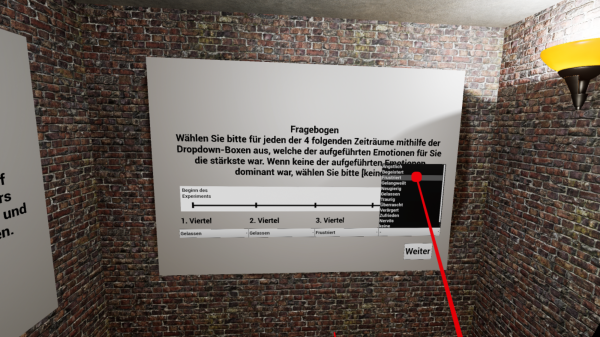
\includegraphics[width=\textwidth]{Images/Fragebogen_1.png} 
\caption{ Bild des Fragebogen-Teils, wo die dominierenden Emotionen abgefragt werden. } 
\label{fig:fragenbogen1} \end{figure}

% Unterkapitel 
\subsection{Szenarien} \label{szenarien-subsec}

\todo[inline]{Verantwortlich: Meryem}

% Unterkapitel 
\input{Part-1/3-Emotionsinduktion/3-Szenarien/1-glueck}

% Unterkapitel 
\input{Part-1/3-Emotionsinduktion/3-Szenarien/2-langeweile}

% Unterkapitel 
\input{Part-1/3-Emotionsinduktion/3-Szenarien/3-frust}


% 4 Messreihe
\newpage
\section{Messreihe} \label{messreihe-4}
\todo[inline]{Kevin, Artur}




% 5 Mustererkennung
\newpage
\section{Mustererkennung} \label{mustererkennung-4}

\todo[inline,color=green!40]{Verantwortlich: Artur\\
- RfP}

In diesem Kapitel werden alle Schritte entlang der ERC (vgl. Kapitel \ref{emotion-recogniton-chain}) konkretisiert und es wird detailreich beschrieben, wie wir vorgegangen sind. \\


% 1 Datenerfassung
\subsection{Datenerfassung} \label{datenerfassung-1}


In Kapitel \ref{messreihe-1-sec} wurde das verwendete Datenset bereits detailiert beschrieben, sodass hier darauf verzichtet wird. \\

% 2 Vorverarbeitung
\subsection{Vorverarbeitung} \label{vorverarbeitung-1}

Wie bereits in Kapitel \ref{vorverarbeitung-0} beschrieben, ist das Ziel der Vorverarbeitung die ”Verbesserung” der Daten f{\"u}r die nachfolgenden Schritte der ERC.
Im Rahmen des ELISE Projektes wurden Normalisierungstechniken auf dem gesamten Datensatz angewendet. 
Wir haben insbesondere die Standardnormalisierung verwendet, welche den Mittelwert der Daten auf Null setzt und die Einheitsvarianz ergibt \cite{grus15}. 
Die Formel f{\"u}r die Standardnormierung lautet:
\begin{equation} 
\Large{ {x'={\frac {x-{\overline {x}}}{\sigma }}} } 
\label{equ:norm} \end{equation} %\vspace{0.5cm}

wobei $ x $ ein Datenpunkt eines Sensorkanales, $ \overline{x} $ ist der Durchschnitt der Gesamtheit f{\"u}r diesen Sensorkanal und $ \sigma $ ist die entsprechende Standardabweichung. \\

% 3 Segmentation
\subsubsection{Segmentation} \label{segmentation-0}

Ziel dieses Schrittes ist es, Teile von Daten zu identifizieren, welche wichtige Informationen über die zu erkennenden Emotionen enthalten. 
Dies geschieht durch Filtern der Daten und Ausschließen von Segmenten, die für das Klassifizierungsproblem nicht relevant sind.
Zusätzlich wird die zu verarbeitende Datenmenge reduziert, indem Segmente eines Zeitfensters fester Größe aus den Daten extrahiert werden.
Diese Vorgeheisweise ist heute in der Praxis besonders wichtig, da sonst hardwarebedingte Einschränkungen die zu verarbeitende Datenmenge begrenzen könnten. \\

% 4 Merkmalsextraktion
\subsection{Merkmalsextraktion} \label{merkmalsextraftion-1}

Wie bereits in Kapitel \ref{merkmalsextraktion-subsubsec} beschrieben, ist das Ziel der Merkmalsextraktion Charakteristiken und Merkmale in den Daten zu finden, die für das
Klassifizierungsproblem von möglichst hoher Relevanz sind. Im Rahmen des ELISE Projektes haben wir verschiedene Vorgehensweisen angewendet. Im den folgenden Unterkapiteln werden diese vorgestellt. \\



% Unterkapitel 
\subsubsection{Handgefertigte Merkmale} \label{hc-features-1}
Der handgefertigten Merkmal Ansatz (enlg. "hand-crafted features approach") besteht in der Berechnung relativ einfacher Merkmale von denen vermudetet wird, dass sie für das Klassifizierungsproblem der Eingangssignale relevant sein können. Diese Vorgehensweise hat den Vorteil des einfachen Aufbaus als auch der relativ geringen benötigten Rechenleistung, wobei potentiell gute Klassifizierungsergebnisse erwarten werden. \\


Obwohl frühere Forschungsarbeiten schon handgefertigte Merkmale zur Emotionserkennung unter mithilfe physiologischer Signale getestet haben (vgl. \cite{martinez_ieee_2013}), wurde dieser Ansatz noch nie für die Erkennung dieser spezifischen Emotionen unter Verwendung dieser Kombination von Sensoren getestet.
Zusätzlich haben wir zuerst handgefertigte Merkmale getestet, um ein Basisergebnis zu liefern, mit der die Ergebnissen der anderen Ansätze vergleichen werden können.
Handgefertigte Merkmale sind in der Regel entweder einfache statistische Werte, Fourier-basierte oder selbstentwickelte Merkmale sein, die aufgrund von Vorkenntnissen der Daten verwendet werden. 
Diese Arbeit wurden statistische, Fourier-basierte und selbstentwickelte Merkmale getestet. \\

\textbf{Statistische Merkmale \\}
Die Tabelle \ref{tab:statistische} fasst die elf verschiedenen und in der Studie verwendeten statistischen Merkmale zusammen. Wir bezeichnen $\mathbf{x} = (x_1, x_2, ...., x_T) $ als Vektor, der die in einem Datenzeitfenster der Länge $T$ enthaltenen Sensorwerte für einen Sensorkanal darstellt. 


\begin{table}[h]
\begin{tabular}{| l | p{12.5cm} |}
\hline
    \textbf{Merkmalname}     &  \textbf{Definition}  \\ \hline
    
    Durchschnitt         & \vspace{0.01cm}
    $ mean(\mathbf{x}) =$ \Large{$\frac{1}{T} \sum_{k=1}^T (x_k) $} \\[0.5cm] \hline 
    
    Standard-Abweichung        & \vspace{0.01cm}
    $ \sigma(\mathbf{x}) =$ \Large{$ \sqrt{ \frac{1}{T} \sum_{k=1}^{T}{(x_k - \mu)^{2}} } $ } \\[0.5cm] \hline
    
    Maximum                   & \vspace{0.01cm}
    $ max(\mathbf{x}) = \max(x_{1},x_{2},\dots ,x_{T}) $
    \\[0.5cm] \hline
    
    Minimum                   & \vspace{0.01cm}
    $ min(\mathbf{x}) = \min(x_{1},x_{2},\dots ,x_{T}) $
    \\[0.5cm] \hline
    
    Amplitude                 & \vspace{0.01cm}
    $ A(\mathbf{x}) = max(\mathbf{x}) - min(\mathbf{x}) $ 
    \\[0.5cm] \hline
    
    25/50/75\% Perzentil      & Wert einer Menge, unter dem 25/50/75\% der Werte aus der Menge fallen. \\ \hline
    
    Interquartiler Bereich    & Differenz zwischen dem 75. und 25. Perzentil.
    \\ \hline
     
    Schräge                   & \vspace{0.01cm}
    $ \gamma _{1}(\mathbf{x}) = \operatorname{E}$ \Large{$\left[\left({\frac {X-\mu }{\sigma }}\right)^{3}\right]$ \normalsize{$=$} ${\frac {\mu _{3}}{\sigma ^{3}}}$ \normalsize{$=$} ${\frac {\operatorname {E} \left[(X-\mu )^{3}\right]}{ (\operatorname {E} \left[(X-\mu )^{2}\right])^{3/2}}}$ \normalsize{$=$} ${\frac {\kappa _{3}}{\kappa _{2}^{3/2}}} $} \vspace{0.2cm}
    \\[0.3cm] \hline
     
    Kurtosis                  & \vspace{0.01cm}
    $ \operatorname {Kurt}[\mathbf{x}] = \operatorname{E} $ \Large{$\left[\left({\frac {X-\mu }{\sigma }}\right)^{4}\right]$ \normalsize{$=$} ${\frac {\mu _{4}}{\sigma ^{4}}}$ \normalsize{$=$} ${\frac {\operatorname {E} [(X-\mu )^{4}]}{(\operatorname {E} [(X-\mu )^{2}])^{2}}} $} \vspace{0.2cm}
    \\[0.3cm] \hline
\end{tabular} 
\caption{Statistische Merkmale, die im Rahmen des ELISE-Projektes verwendet wurden. } \label{tab:statistische}
\end{table} 


\textbf{Fourier-basierte Merkmale \\}
\todo[inline]{Artur: \\
- Muss ich noch schreiben $\rightarrow$ Warten auf Julian's Antwort. \\}


\textbf{Selbstentwickelte Merkmale \\}
Es wurden zwei eigene Merkmale definiert: Nulldurchgang (engl. "zero crossing") und Anzahl der Spitzen (engl. "number of peaks"). Im Folgendem werden diese beiden Merkmale detailiert beschrieben. \\

Das Nulldurchgang-Merkmal zählt die Häufigkeit, mit der das Signal eines Sensorkanals in einem Zeitfenster die Nulllinie überschreitet.
Alle Sensorsignale wurden durch Normierung verarbeitet (vgl. Kapitel xxx) und damit wurden alle Mittelwerte auf Null zentriert.
Um zu vermeiden, dass Rauschen entlang der Nulllinie in dem Merkmal gezählt wird, wird nur ein Nulldurchgang in einer bestimmten Zeitspanne gezählt. \\


Das Spitzenzähler-Merkmal bestimmt die Anzahl von loklanen Hochpunkten im Zeitsignal.
Alle lokalen Maximen sind durch einen Onset (Startpunkt), eine Spitze und einen Offset (Endpunkt) gekennzeichnet (vgl. Abbildung \ref{fig:peaks}). 
Jedes Vorkommen einer Onset/Offset-Paarung wird hierbei als Spitze gezählt.
Onsets, Spitzen und Offsets werden durch die folgenden Operationen identifiziert \cite{BSc_Gouverneu}:

\begin{itemize} %[noitemsep]
  \item Ein Onset wird bestimmt, wenn der Wert des Signals an diesem Punkt nicht negativ ist und die Differenz zwischen ihm und dem nächsten größer als ein vordefinierter Schwellenwert (engl. "threshold") ist.

  \item Ein Offset wird bestimmt, wenn der Wert des Signals kleiner als der Wert des zuletzt gesetzten Onsets ist.

  \item Das lokale Maximum zwischen einem Onset und Offset wird als Spitze bezeichnet.
\end{itemize} \vspace{0.2cm}


\begin{figure}[h] \centering{
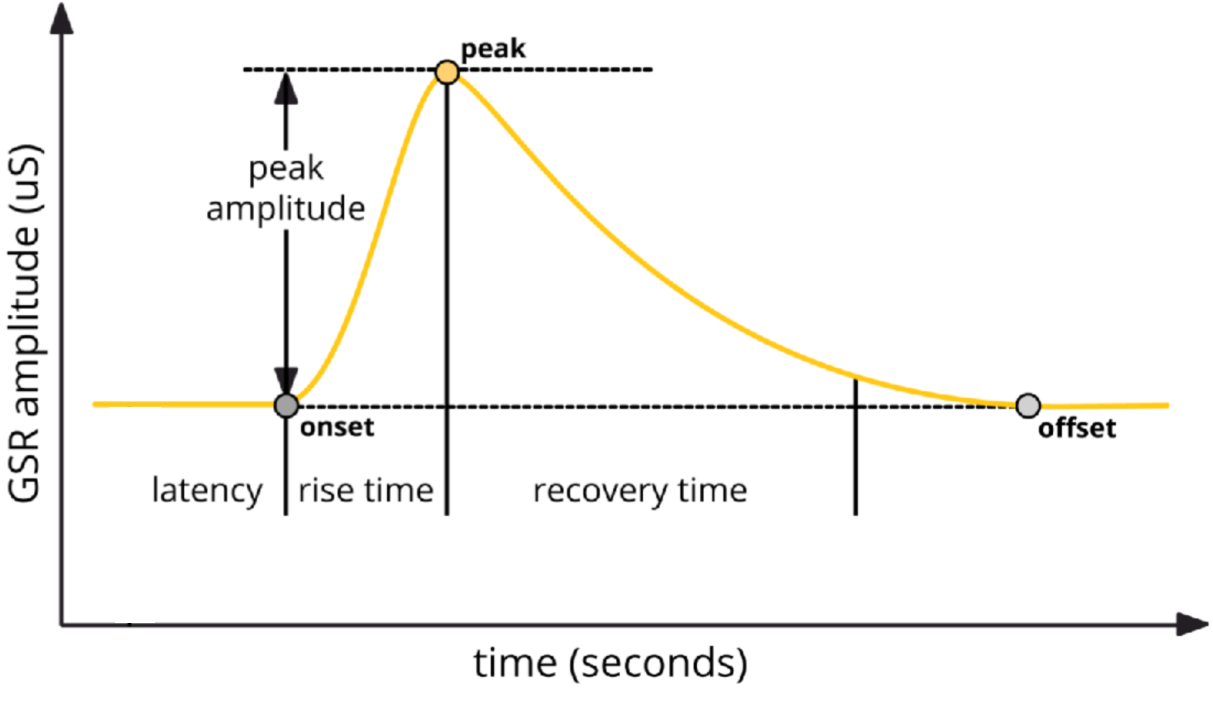
\includegraphics[width=11cm]{Images/peaks.png}}
\caption{ Spitzenzähler: Onset (Startpunkt), Spitze und Offset (Endpunkt). Jedes Paar von Onset/Offset erhöht die Anzahl der Spitzen um eins.} 
\label{fig:peaks} \end{figure} \vspace{0.5cm}


Jedes handgefertigte Merkmal wird auf einem Zeitfenster von Daten für jeden Sensorkanal unabhängig voneinander angewendet. 
Jedes Zeitfenster ist daher 117 Merkmalen zugeordnet (9 Sensorkanäle multipliziert mit 13 Merkmalen). \\





% Unterkapitel 
\subsubsection{Codebook Approach} \label{ca-1}


Die bisherige Methodik mit handgefertigten Merkmalen ist klassisch für den überwachten Lernansatz. 
Es existieren aber auch einige Nachteile. 
Das Hauptproblem besteht darin, dass nicht sichergestellt werden kann, dass die gewählten Merkmale die besten Klassifizierungsergebnisse erzielen. Damit besteht immer die Gefahr, dass möglicherweise andere Merkmalen bessere Ergebnisse liefern würden, diese handgefertigten Merkmale aber die  nicht gefunden wurden. Dieses Risiko besteht insbesondere bei der physiologischen Signalverarbeitung zur Emotionserkennung, wo die Struktur der Daten noch recht unbekannt und allgemein komplex ist. 
Eine weitere Schwierigkeit besteht darin, relevante selbstentwickelte Features ohne Expertenwissen über die Daten zu finden.
Darüber hinaus wurden noch keine gut funktionierenden State-of-the-Art handgefertigten Merkmale identifiziert.
Aus diesen Gründen ist es interessant halbautomatische und unüberwachter Ansätze der Merkmalsextraktion zu verwenden und zu testen. \\


K. Shirahama et al. \cite{kimiaki_codebook_approach_2016} schlugen eine unüberwachte Merkmalsextraktionsmethode namens Codebook Approach (CA) vor, um Merkmale aus 1D-Zeitreihensignalen zu erzeugen.
Der CA hat den Vorteil, dass formbasierte Merkmale gefunden werden können, die für das Problem der Emotionserkennung relevant sind, aber weder offensichtlich noch leicht als Mensch zu interpretieren sind. 
Der CA besteht aus drei Schritten, die in den folgenden Abschnitten erläutert werden: Codebuchkonstruktion (engl. "codebook construction"), Codewortzuordnung (engl. "codeword assignment") und der anschließenden Klassifizierung. \\


\textbf{Codebuchkonstruktion \\}
Ziel dieses Schrittes ist es, Teilsequenzen (sogenannte "Codewörter") zu bestimmen, die für die 1D-Eingangssensorik charakteristisch sind. 
Dies wird erreicht, indem Zeitfenster aus dem ursprünglichen Datensatz für jeden Sensorkanal unabhängig voneinander nach dem im Kapitel \ref{segmenation-1} definierten Segmentierungsansatz extrahiert werden.
Aus jedem so erhaltenen Zeitfenster der Größe $T$ werden kleinere Segmente der Größe $\alpha$ unterteilt.
Ein Clustering-Algorithmus wird dann auf die Menge der Segmente $\alpha$ angewendet, um Clusterzentren zu finden.
Nach der Konvergenz werden die Clusterzentren als Codewörter betrachtet und zum Aufbau einer Sammlung von Codewörtern mit dem Namen ``Codebuch'' verwendet, wie in Abbildung \ref{fig:ca_construction} aus \cite{kimiaki_codebook_approach_2016} dargestellt. 
Die Anzahl der Codewörter (d.h. die Größe des Codebuchs oder die Anzahl der Cluster) ist ein Hyperparameter des Verfahrens. Im Rahmen dieser Arbeit wurde ein k-means Clustering-Algorithmus verwendet, um die Codewörter auf den ELISE-Daten zu erhalten. \\



% 5 Klassifikation
\subsection{Klassifikation} \label{klassifikation-1}

Wie bereits in Kapitel \ref{grundlagen-klassifikation-0} beschrieben ist das Ziel der Klassifizierung ein Klassifizierungsmodell zu trainieren, das in der Lage ist, Objekte in den Daten in die entsprechende Klasse zuzuordnen. Die Klassen entsprechen hierbei den Emotionen, die erkannt werden sollen: Glück, Langeweile, Frustation und andere (d.h. alle Emotionen, die nicht Glück, Langeweile oder Furstation entsprechen). \\

Als erstes wird der Datensatz in ein Trainigs- und Testset  aufgeteilt. 
Es gibt keine festgelegten Regeln über die Proportionen der Sets. 
Im Allgemeinen wird das Trainingsset aber größer als das Testset gewählt.
Da die Leistungen des Klassifikators jedoch stark von der gewählten Aufteilung abhängen, ist es wichtig, sicherzustellen, dass dieser Schritt richtig durchgeführt wird.
Bei einem Datensatz mit mehreren Probanden empfiehlt sich für die Aufteilung zwischen Trainings- und Testsets die Durchführung einer Leave-One-Subjekt-Out-Cross-Validierung (LOSOCV).
Die Idee besteht darin, $N$ verschiedene Aufteilungen des Datensatzes vorzunehmen, wobei $N$ die Anzahl der Personen ist, die Daten für den Datensatz bereitgestellt haben. 
Für jeden dieser Splits wird der Testset aus den Daten eines Probanden aufgebaut, während die Daten der anderen Probanden das Trainingsset bilden. 
Anschließend wird ein Klassifizierer erstellt und ausgewertet. Dies wird für alle Probanden wiederholt, d.h. $N$ mal.
Die so erhaltenen $N$-Bewertungskennzahlen (eine pro Proband) können dann gemittelt werden, um eine Gesamtbewertung des Modells zu erhalten.
Es ist wichtig zu beachten, dass der LOSOCV-Ansatz bei einer hohen Anzahl von Probanden sehr rechenintensiv sein kann. \\

\begin{figure}[h] \centering{
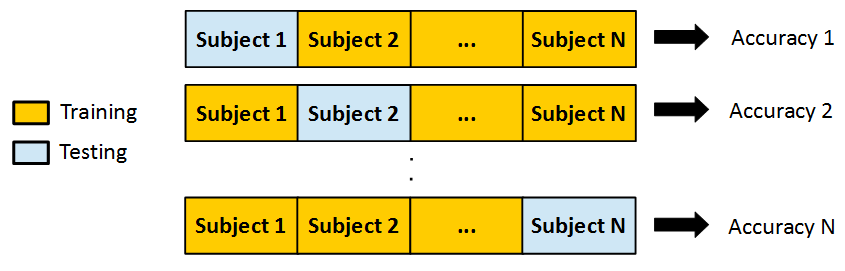
\includegraphics[width=15cm]{Images/LOSOCV.png} 
\caption{ Leave-One-Subjekt-Out-Cross-Validation (LOSOCV): $N$ entspricht der Anzahl der Probanden. Für jeden Split wird ein Testset aus den Daten eines Probanden aufgebaut, während die Daten der anderen Probanden einen Trainingsset bilden. Dieser Vorgang wird für die Daten jedes Probanden durchgeführt. }}
\label{fig:losocv} \end{figure} \vspace{0.5cm}

% 6 Ergebnisse
\newpage
\section{Ergebnisse} \label{ergenisse-4}
\todo[inline]{Artur}



% Unterkapitel 
\subsubsection{Hand-gefertigte Merkmale} \label{hc-features-subsubsec}







% Unterkapitel 
\subsection{Ergebnisse des Codebook Approach} \label{ergebnisse-codebook-approach-subsec}


{\"A}hnlich wie bei den handgefertigten Merkmalen haben wir die Daten mit einer Normalisierungstechnik vorverarbeitet und dann die Segmentierung verwendet. Die Zeitfensterparameter sind identlisch wie bei der Studie mit den handgefertigten Merkmalen.
F{\"u}r die Klassifizierung haben wir SVM mit Soft-Margins und dem RBF-Kernel benutzt. 
Um die optimalen Parameter des SVM-Klassifikators zu bestimmen (z.B. Soft-Margin $C$ und Kernelparameter $\gamma$), wurde hier wieder die Gitter-Suche angewendet. \\


Die Ergebnisse, die wir mit dem CA mit fester Zuordnung (hard assignment) und $C = 8$, $\gamma = 0,002$ f{\"u}r jeden Probanden erhielten, waren 52\%, 38\% und 38\%, was einem Durchschnitt von 42,67\% entspricht. CA mit Soft-Assignment wurden ebenfalls getestet, lieferte aber schlechtere Ergebnisse als CA mit Hard-Assignment. In diesem speziellen Datensatz schneidet der CA also schlechter ab als die handgefertigten Merkmale.








\subsection{Ergebnisse der Deep Neutral Networks} \label{ergebnisse-dnn}

Die Verwendung von DNNs zur Extraktion von Merkmalen (z.B. Multi-Layer-Perceptron, Convolutional Neural oder Long-Short-Term-Memory Networks) wurden zwar intensiv getestet (siehe \cite{bscschnieber18}), diese Ansätze erreichten aber leider nicht so gute Ergebnisse, wie z.B. die oben vorgestellten Ergebisse der handgefertigten Merkmale. Die beste Performance erreichten LSTM mit einem F1-Score von 47,99\%. \\



% Unterkapitel
\subsection{Analyse der Ergebnisse} \label{analyse-subsec}










% 7 Alternativen
\newpage
\section{Alternative Lösungen} \label{alternativen-4}
\todo[inline]{Verantwortlich: Artur}

Da davon ausgegangen wird, dass weder Codebook Approach noch die handgefertigten Merkmale die ernüchternden Ergebnisse der DNN übertreffen können, wurde stattdessen nach alternativen Lösungsmöglichkeiten gesucht.
Im folgenden werden die beiden vielversprechendsten Optionen vorgestellt.



% Unterkapitel 
\subsection{Kalibrierung} \label{kalibrierung-4}

\todo[inline]{Verantwortlich: Jonas}
Um die Präzision der vorhergesagten Emotionen weiter zu verbessern, wurde statt eines generellen Modells für alle Subjekte, der Ansatz eines personalisierten Modells geprüft. Dabei werden in einer kurzen Trainingsphase die Daten und Labels der Versuchsperson genutzt um das ML Modell zu trainieren, der Unterschied zum generalisieten Ansatz besteht hierbei, dass die charakteristischen Eigenschaften der Biosignale des Subjektes nicht über Vermischung mit denen der anderen Subjekte gemittelt werden, sondern zur Bestimmung des emotionalen Zustandes heran gezogen werden können. Die Gültigkeit des Modells beschränkt sich dabei auf die Testperson, für die das Modell gebildet wurde. Zur Validierung des Erfolges der Kalibrierung erfolgt nach der Trainingsphase eine Validierungsphase in der die Gültigkeit und die Präzision gemessen wird. \\

Zur Umsetzung wurde ein weiteres VR Emotionsinduktionsszenario erstellt. Hierbei werden in VR der Testperson auf einer virtuellen Leinwand 60 sekündige Videoausschnitte gezeigt und danach nach der Einschätzung des emotionalen Zustandes nach dem Circumplex Modell gefragt. Hierbei werden die gleichen Fragebögen wieder verwendet, die auch in der Hauptinduktion Verwendung finden (siehe. Abbildung \ref{fig:ablauf_kalibrierung}). Die Auswahl der Videos erfolgt dabei vor allem aus dem DEAP Datensatz (vgl. \cite{}). Dieser wurde insbesondere für die Validierungsphase mit weiteren Videosequenzen angereichert, deren Auswahl den gleichen Kriterien unterlag wie für den DEAP Datensatz. \\

Ausgewählt wurden für die beiden Kategorien Arousal und Valence jeweils drei Videos mit einem hohen und drei Videos mit einem niedrigen Wert. Insgesamt ergibt das für die Trainingsphase 12 Videos (3 Arousal hoch, 3 Arousal niedrig, 3 Valence hoch, 3 Valence niedrig). Diese Videos werden randomisiert hintereinander gezeigt. Damit ergibt sich eine Gesamtlaufzeit für ein Kalibrierungstraining von 15 bis 20 Minuten.  Nach dieser Zeit wartet der Proband, bis das ML Modell vollständig trainiert wurde, direkt in Anschluss daran werden ihm dann die 4 Validierungsvideos wieder randomisiert zwischen den vier Ausprägungen von Arousal und Valence gezeigt. Hierbei wird der emotionale Zustand des Probanden auch wieder nach jedem Video mit einem Fragebogen evaluiert. Anschließend erfolgt eine Auswertung mittels der Berechnung von Präzision und Recall des ML Modells. Diese Daten werden auch wieder innerhalb des Netzwerkes mittels UDP Paketen publiziert. \\
\begin{figure}[h]
    \centering
\begin{minipage}[t]{0.9\textwidth}
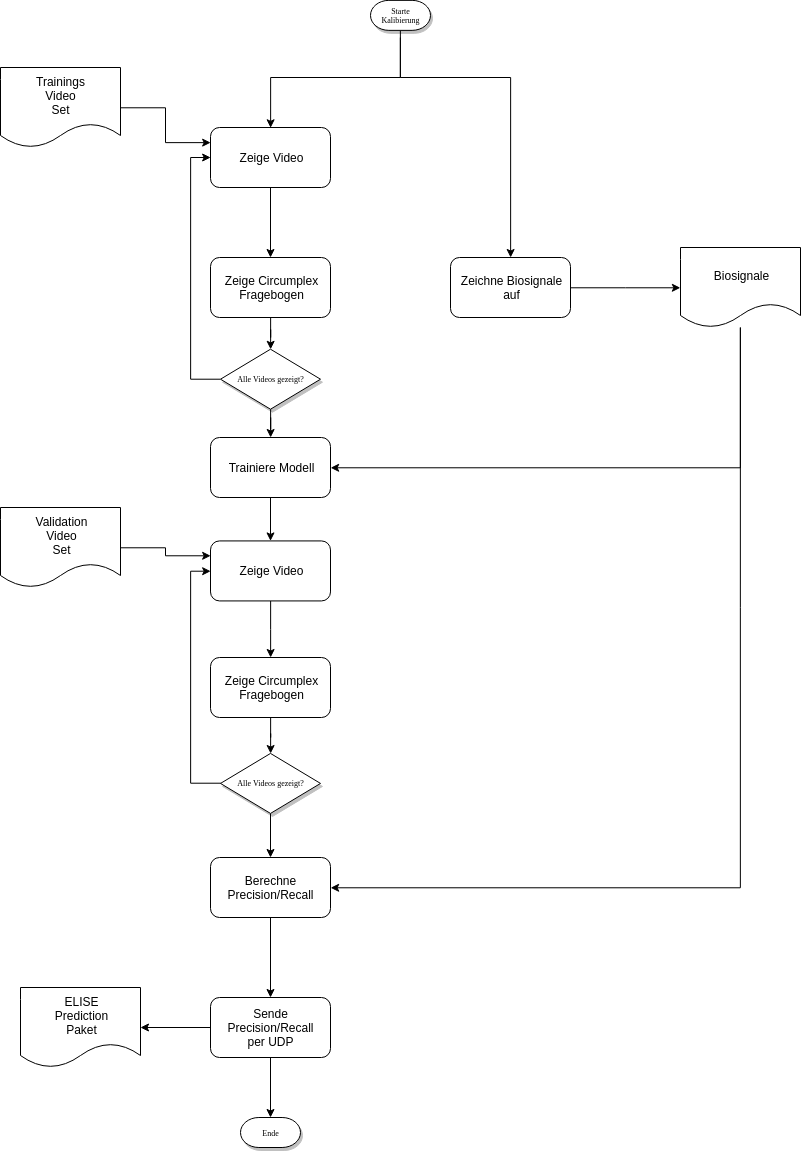
\includegraphics[width=\textwidth]{Images/kalibrierung_ablauf.png}
\end{minipage}
    \caption{Schematischer Ablauf der Kalibrierung}
    \label{fig:ablauf_kalibrierung}
\end{figure}








% Unterkapitel 
\subsection{Plan B} \label{plan-b-4}

\todo[inline]{Verantwortlich: Meryem}











% Part 5 - Schlussteil
\newpage
\pagestyle{fancy} \fancyhf{} \rhead{\leftmark} \cfoot{\thepage} % Header Part 5
\section{Zusammenfassung und Ausblick} \label{ende-sec}


In diesem Kapitel wird die Zusammenfassung der Arbeit sowie das resultierende Fazit und schlie{\ss}lich ein Ausblick dargeboten.


% Unterkapitel
\subsection{Zusammenfassung} \label{zusammenfassung-subsec}







% Unterkapitel
\subsection{Ausblick} \label{ausblick-subsec}











% List of Figures
\newpage 
\pagestyle{plain} % Header entfernen
\renewcommand{\listfigurename}{Abbildungsverzeichnis}
\addcontentsline{toc}{section}{Abbildungsverzeichnis}
\listoffigures


% List of Tables
\newpage
\renewcommand{\listtablename}{Tabellenverzeichnis}
\addcontentsline{toc}{section}{Tabellenverzeichnis}
\listoftables


% Abkuerzungen
\newpage

\section*{Abkürzungen}
\addcontentsline{toc}{section}{Abkürzungen}

\noindent
\todo[inline]{Bitte alle verwendete Abkürzungen nochmals hier aufführen.}

\begin{acronym}[LOSOCV]
 \acro{ANN}{Artificial Neural Networks}
 \acro{BMBF}{Bundesministerium für Bildung und Forschung}
 \acro{BVP}{Blood Volume Pulse}
 \acro{CA}{Codebook Approach}
 \acro{CRID}{Center for Responsible Innovation \& Design}
 \acro{C-SVM}{Soft-margin Support-Vector-Machine}
 \acro{CSV}{Comma-Separated-Values}
 \acro{DDS}{Direct Draw Surface}
 \acro{EEG}{Electroencephalography}
 \acro{EOG}{Electrooculography}
 \acro{ERC}{Emotion Recognition Chain}
 \acro{GSR}{Galvanic Skin Response}
 \acro{HR}{Heart Rate}
 \acro{LOSOCV}{Leave-One-Subject-Out-Cross-Validation}
 \acro{PG}{Projektgruppe}
 \acro{PPG-ir}{Photoplethysmography Infrared}
 \acro{PPG-red}{Photoplethysmography Red}
 \acro{RBF}{Radial Basis Function}
 \acro{SpO2}{Pulse Oximetry}
 \acro{SVM}{Support-Vector-Machine}
 \acro{VR}{Virtual Reality}
\end{acronym}



% Referenzen
\newpage
\bibliographystyle{plain}
\bibliography{References/artur}


% Anhang
\newpage
\section*{Anhang}
\addcontentsline{toc}{section}{Anhang}

% Hier Gliederung / Inhaltverzeichnis des Anhangs.

\end{sloppypar}
\end{document}